% -------------------------------
% Plantilla del TFG en la ESIIAB-UCLM. Versión 0.0 (Preliminar)
%
% Luis de la Ossa
% 
% Compilar con XeLaTeX 
% -------------------------------
\documentclass[12pt, a4paper]{book}

% -------------------------------
% Información y opciones del documento. Debe editarse.
% -------------------------------
% -------------------------------
% Plantilla del TFG en la ESIIAB-UCLM. Versión 0.0 (Preliminar)
%
% Luis de la Ossa
% 
% Compilar con XeLaTeX 
% -------------------------------


% -------------------------------
% Comandos comunes
% -------------------------------
\newcommand{\uclm}{Universidad de Castilla-La Mancha\,}
\newcommand{\dsi}{Departamento de Sistemas Informáticos\,}
\newcommand{\esii}{Escuela Superior de Ingeniería Informática de Albacete\,}
\newcommand{\iiia}{Instituto de Investigación en Informática de Albacete\,}


% -------------------------------
% Comandos específicos
% -------------------------------
\newcommand{\autor}{Pablo Valiente Martínez\,}
\newcommand{\titulo}{Estudio comparativo de sistemas de ficheros basados en Linux\,}
\newcommand{\director}{Gabriel Cebrián Marquez\,}
\newcommand{\codirector}{Valentín Valero Ruiz\,}
\newcommand{\fecha}{Mayo, 2023\,}
 \newcommand{\espec}{Ingeniería de Computadores\,} 







% -------------------------------
% Configuración del documento, paquetes, etc.
% -------------------------------
% -------------------------------
% Plantilla del TFG en la ESIIAB-UCLM. Versión 0.0 (Preliminar)
%
% Luis de la Ossa
% 
% Compilar con XeLaTeX 
% -------------------------------

% -------------------------------
% Idioma
% -------------------------------
\usepackage{polyglossia}
\setmainlanguage{spanish}

% -------------------------------
% Fuente
% -------------------------------
% Cualquier tamaño de texto: {\fontsize{100pt}{120pt}\selectfont tutexto}
\usepackage{anyfontsize}
% Selección de fuentes.
\usepackage{fontspec}
% Espacio entre líneas
\usepackage{setspace}
% Fuentes especiales
\usepackage{textcomp,marvosym,pifont}

\usepackage{tcolorbox}
\usepackage[all]{nowidow}
\usepackage{microtype}
\usepackage{pgfplots}
\usepackage{filecontents}
\usepackage{longtable}



% -------------------------------
% Otros paquetes de uso común
% -------------------------------
% Símbolos matemáticos
\usepackage{amsmath,amsfonts,amssymb}
% Gráficos
\usepackage{graphicx}
% Posición arbitraria de los gráficos
\usepackage[absolute,overlay]{textpos}
% Apéndices
\usepackage{appendix}

% -------------------------------
% Esquema de colores
% -------------------------------
% Paquete para la definición de colores
\usepackage[table]{xcolor}
% Esquema de colores
% -------------------------------
% Plantilla del TFG en la ESIIAB-UCLM. Versión 0.0 (Preliminar)
%
% Luis de la Ossa
% 
% Compilar con XeLaTeX 
% -------------------------------

% -------------------------------
% Color del tema
% -------------------------------

% Color para los títulos, etc.
%\definecolor{tema}{RGB}{0,0,0}        % Negro 
%\definecolor{tema}{RGB}{182,0,52}     % LOGO UCLM
\definecolor{tema}{RGB}{0,69,134}      % Azul del esquema  
%\definecolor{tema}{RGB}{197,0,11}     % Rojo del esquema     

% Negritas con el color del tema
\newcommand{\bft}[1]{\textcolor{tema}{\bf #1}} 


% -------------------------------
% Esquema de colores
% -------------------------------
% Estos balores coinciden con colores de OpenOffice 
% Se pueden redefinir para que coincidan con las paletas de las 
% herramientas utilizadas para hacer las gráficas.
\definecolor{blanco}{RGB}{255,255,255} 
\definecolor{negro}{RGB}{0,0,0}
\definecolor{gris95}{gray}{.95}
\definecolor{gris75}{gray}{.75}
\definecolor{gris50}{gray}{.50}
\definecolor{gris25}{gray}{.25}
\definecolor{rojo}{RGB}{197,0,11}        % Gráfico 11
\definecolor{azul}{RGB}{0,69,134}        % Gráfico 1
\definecolor{verde}{RGB}{87,157,28}      % Gráfico 4
\definecolor{naranja}{RGB}{255, 149, 14} % Gráfico 10
\definecolor{mostaza}{RGB}{255, 211, 32} % Gráfico 3

% Negrita con color definido 
\newcommand{\bfa}[1]{\textcolor{azul}{\bf #1}} 
\newcommand{\bfr}[1]{\textcolor{rojo}{\bf #1}}
\newcommand{\bfn}[1]{\textcolor{naranja}{\bf #1}}
\newcommand{\bfv}[1]{\textcolor{verde}{\bf #1}}  
\newcommand{\bfm}[1]{\textcolor{mostaza}{\bf #1}} 





% -------------------------------
% Márgenes
% -------------------------------
% Márgenes de las páginas
\usepackage[
  inner  =  3cm,   % Margen interior
  outer  =  2.5cm, % Margen exterior
  top    =  2.5cm, % Margen superior
  bottom =  2.5cm, % Margen inferior
  includeheadfoot, % Incluye cabecera y pie de página en los márgenes
]{geometry}
% Muestra una regla para comprobar el formato de las páginas (descomentar)
%\usepackage[type=upperleft,showframe,marklength=8mm]{fgruler} 

% -------------------------------
% Renombra tablas y bibliografía
% -------------------------------
\addto\captionsspanish{
    \renewcommand{\listtablename}{Índice de tablas} 
    \renewcommand{\tablename}{Tabla}
    \renewcommand{\bibname}{Referencia bibliográfica}
}

% -------------------------------
% Itemize y enumerate. Control de los espacios.
% -------------------------------
\usepackage{enumitem}
\setitemize{itemsep=0pt}
\setenumerate{itemsep=0pt}
\renewcommand{\labelitemi}{\tiny\bft{$\blacksquare$}}
\renewcommand{\labelitemii}{\bft{$\bullet$}}
\renewcommand{\labelitemiii}{\bft{-}}

% -------------------------------
% Enlaces y colores
% -------------------------------
\usepackage{hyperref}
%\hypersetup{
%    colorlinks,
%    citecolor=black,
%    filecolor=black,
%    linkcolor=black,
%    urlcolor=black
%}

% -------------------------------
% Gestión de elementos flotantes
% -------------------------------
% Para forzar a que las figuras aparezcan antes del fin de una sección.
%\usepackage[section]{placeins}

% Gestión de títulos de los elementos flotantes
\usepackage{caption}
% Subfiguras y títulos en subfiguras
\usepackage{subcaption}

% Títulos
\DeclareCaptionFont{tema}{\color{tema}} % Color
\captionsetup{labelfont={tema, bf}}     % Estilo
\captionsetup{font=normalsize}          % Tamaño
\captionsetup{width=.9\linewidth}       % Anchura del título
% Distancia de la figura al texto.
\setlength{\intextsep}{1cm} 
\setlength{\textfloatsep}{1cm}         

% -------------------------------
% Utilidades para tablas
% -------------------------------
% Para fundir filas en tablas
\usepackage{multirow}
% Para definir columnas con ancho fijo y alineación
\usepackage{array,ragged2e}
\newcolumntype{L}[1]{>{\raggedright\let\newline\\\arraybackslash\hspace{0pt}}m{#1}}
\newcolumntype{C}[1]{>{\centering\let\newline\\\arraybackslash\hspace{0pt}}m{#1}}
\newcolumntype{R}[1]{>{\raggedleft\let\newline\\\arraybackslash\hspace{0pt}}m{#1}}

% -------------------------------
% Para tabular
% -------------------------------
\usepackage{tabto}

% -------------------------------
% Formato de títulos, capítulos, etc.
% -------------------------------
\usepackage{titlesec, titletoc}
% Parte
\titleformat{\part}[display]                                                     % Estilo
    {\Huge \centering \color{tema}}                                                % Formato
    {Parte \thepart }                                                              % Etiqueta
    {0.75ex}                                                                       % Separación
    {\bfseries\fontsize{25pt}{40pt}\selectfont}                                    % Entre etiqueta y título            
    [\thispagestyle{empty}]                                                        % Después

% Capítulo        
\titleformat{\chapter}[block]                                                     % Estilo      
    {\vspace{0cm} \flushright \bfseries \LARGE \color{tema}}                      % Formato 
    {\thechapter.}                                                                % Etiqueta
    {0.75ex}                                                                      % Separación
    {}                                                                            % Entre etiqueta y título
    [\vspace{0.1cm} \rule{0.5\textwidth}{1pt}\vspace*{1cm}\thispagestyle{plain}]  % Después      

% Sección
\titleformat{\section}
    {\vspace{5pt}  \Large \color{tema}}
    {\thesection .}
    {0.75ex}
    {}

% Subsección
\titleformat{\subsection}
    {\large \color{tema}}
    {\thesubsection .}
    {0.75ex}
    {}

% Subsubsección
\titleformat{\subsubsection}
    {\bf\color{tema}}
    {}
    {0.75ex}
    {}

% Parte (TOC)
\titlecontents{part}[2pc]
      {\vspace{20pt}\bfseries\filright\Large\color{tema}}
      {\contentslabel{1.5pc}}{\hspace*{-1.5pc}}
      {\vspace{5pt}}
      {}

% Capítulo (TOC)
\titlecontents{chapter}[2pc]
      {\vspace{10pt}\bfseries\large\filright}
      {\contentslabel{1.5pc}}{\hspace*{-1.5pc}}
      {\mdseries\titlerule*[0.5pc]{.}\bfseries\contentspage}

% Sección (TOC)
\titlecontents{section}[4pc]
      {\vspace{5pt}\filright}
      {\contentslabel{2pc}}{\hspace*{2pc}}
      {\titlerule*[0.5pc]{.}\contentspage}
      {\vspace{5pt}}

% Subsección (TOC)
\titlecontents{subsection}[6pc]
      {\vspace{2.5pt}\filright\small\em}
      {\contentslabel{3pc}}{\hspace*{-3pc}}
      {\titlerule*[0.5pc]{.}\contentspage} 

% -------------------------------
% Cabeceras y pie de página
% -------------------------------
\usepackage{fancyhdr}
\pagestyle{fancy}
\fancyhf{}

% Permite incluir la parte. Para ello crea \parttitle
\let\Oldpart\part
\newcommand{\parttitle}{}
\renewcommand{\part}[1]{\Oldpart{#1}\renewcommand{\parttitle}{#1}}

% Cabeceras y pies de página
\fancyhead[LE]{}
\fancyhead[RO]{\slshape \leftmark}
\fancyfoot[LE,RO]{\thepage}
\renewcommand{\footrulewidth}{1pt}
\renewcommand{\headrulewidth}{1pt}
\renewcommand{\chaptermark}[1]{\markboth{#1}{}} % Capítulo (Solo texto)
\renewcommand{\chaptermark}[1]{\markboth{\thechapter. #1}{}} % Capítulo (Número y texto)

% Formato plano para las páginas con títulos (solo incluye el pie de página)
\fancypagestyle{plain}{
\fancyhf{}
\fancyhead{}
\fancyfoot[LE,RO]{\thepage}
\renewcommand{\footrulewidth}{1pt}
\renewcommand{\headrulewidth}{0pt}
}

% -------------------------------
% Utilidades
% -------------------------------
% Marcas
\newcommand{\pcite}{\bfr{\large[?]}\,} % Cita pendiente: [?] en rojo y negrita.
\newcommand{\ps}{\bfr{\huge[--}\,} % Pricipio de un bloque en sucio
\newcommand{\fs}{\bfr{\huge--]}\,} % Fin de un bloque en sucio.

% Notas
\usepackage[textsize=tiny,spanish,shadow,textwidth=2cm]{todonotes}

% Para generar textos "random"
\usepackage{lipsum} 

% -------------------------------
% Algoritmos y código
% -------------------------------

% Se definen entornos específicos para algoritmos y código que permiten
% gestionar los títulos de manera similar en ambos casos, y similar al resto
% de elementos flotantes.
\usepackage{newfloat}

\DeclareFloatingEnvironment[ % Algoritmos
  listname = {Índice de algoritmos},
  name = Algoritmo
]{algorithm}

\DeclareFloatingEnvironment[ % Fragmentos de código
  listname = {Índice de listados de código},
  name = Código
]{code}

% Define un estilo para el encabezado de algoritmos y código.
\DeclareCaptionFormat{algcode}{
% OPCIÓN 1 -> Línea debajo del título
\rule{\dimexpr\textwidth\relax}{0.4pt}\vspace{0cm}
#1#2#3
\vspace{-0.2cm}\rule{\dimexpr\textwidth\relax}{0.4pt} % 
% OPCIÓN 2 -> Sin línea debajo del título
%\rule{\dimexpr\textwidth\relax}{0.4pt}\vspace{0cm}
%#1#2#3
}
\captionsetup[algorithm]{format=algcode, width=\linewidth}
\captionsetup[code]{format=algcode, width=\linewidth}

% Opciones específicas para algoritmos.
\usepackage[noend]{algpseudocode}
% Tamaño de letra y separadores
\makeatletter
\renewcommand{\ALG@beginalgorithmic}{\small\hrule\vskip10pt}
\makeatother
% Variables y funciones
\newcommand{\va}[1]{{\it {#1}}}                
\newcommand{\fu}[1]{{\textsc{#1}}}          
% Palabras clave
\renewcommand{\algorithmicrepeat}{\bft{repetir}}
\renewcommand{\algorithmicuntil}{\bft{hasta}}
\renewcommand{\algorithmicend}{\bft{fin}}
\renewcommand{\algorithmicif}{\bft{si}}
\renewcommand{\algorithmicthen}{\bft{entonces}}
\renewcommand{\algorithmicelse}{\bft{si no}}
\newcommand{\algorithmicelsif}{\algorithmicelse\ \algorithmicif}
\newcommand{\algorithmicendif}{\algorithmicend\ \algorithmicif}
\renewcommand{\algorithmicfor}{\bft{para}}
\renewcommand{\algorithmicforall}{\bft{para cada}}
\renewcommand{\algorithmicwhile}{\bft{mientras}}
\renewcommand{\algorithmicdo}{\bft{hacer}}
\renewcommand{\algorithmicprocedure}{\bft{procedimiento}}
\renewcommand{\algorithmicreturn}{\bft{devolver}}
\renewcommand{\algorithmicfunction}{\bft{función}}
\renewcommand{\algorithmicloop}{\bft{iterar}}

% Opciones específicas para código.
\usepackage{listings}
% Aspecto de los listados de código (ejemplo)
% Los colores se han de cambiar y adaptar a los distintos lenguajes de programación.
\lstset{
    language=Python,
    keywordstyle=\bf\color{tema},  
    breaklines=true,    
    basicstyle={\small\ttfamily},
    tabsize=5,
    frame=t % Es importante no cambiar esta opción (es la línea superior) 
}

% -------------------------------
% Caracteres pifont de uso común (con color)
% -------------------------------
\newcommand{\vmarkt}{\textcolor{tema}{\ding{52}} }  % Checked (V) Tema
\newcommand{\vmarkr}{\textcolor{rojo}{\ding{52}} }  % Checked (V) Rojo
\newcommand{\vmarka}{\textcolor{azul}{\ding{52}} }  % Checked (V) Azul

\newcommand{\xmarkt}{\textcolor{tema}{\ding{55}} }  % Checked (X) Tema
\newcommand{\xmarkr}{\textcolor{rojo}{\ding{55}} }  % Checked (X) Rojo
\newcommand{\xmarka}{\textcolor{azul}{\ding{55}} }  % Checked (X) Azul

\newcommand{\lmarkt}{\textcolor{tema}{\ding{46}} }  % Lápiz Tema
\newcommand{\lmarkr}{\textcolor{rojo}{\ding{46}} }  % Lápiz Rojo
\newcommand{\lmarka}{\textcolor{azul}{\ding{46}} }  % Lápiz Azul

\newcommand{\hmarkt}{\textcolor{tema}{\ding{43}} }  % Mano Tema
\newcommand{\hmarkr}{\textcolor{rojo}{\ding{43}} }  % Mano Roja 
\newcommand{\hmarka}{\textcolor{azul}{\ding{43}} }  % Mano Azul 

\newcommand{\fmarkt}{\textcolor{tema}{\ding{220}} }  % Flecha Tema
\newcommand{\fmarkr}{\textcolor{rojo}{\ding{220}} }  % Flecha Roja 
\newcommand{\fmarka}{\textcolor{azul}{\ding{220}} }  % Flecha Azul


\clubpenalty=10000
\widowpenalty=10000

% Paquetes para la bibliografía
\usepackage[backend=biber, style=ieee, url=true, doi=true]{biblatex} 
\addbibresource{bib/ref.bib} % Carga el archivo de referencias

% Documento
\begin{document}

% -------------------------------
% Portada y título
% -------------------------------
% Fuente  de la portada
% \setmainfont[Ligatures={NoRequired,NoCommon,NoContextual}]{Calibri}
% -------------------------------
% Plantilla del TFG en la ESIIAB-UCLM. Versión 0.0 (Preliminar)
%
% Luis de la Ossa
% 
% Compilar con XeLaTeX 
% -------------------------------
\pagestyle{empty}
\begin{titlepage}\null



\begin{textblock*}{\paperwidth}(0cm,3cm)
\begin{center}

\includegraphics[width=4cm]{figs/logoconciti.png}
\end{center}
\end{textblock*}


\begin{textblock*}{\paperwidth}(0cm,8cm) 
\begin{center}\doublespacing
{\fontsize{16pt}{2pt}\selectfont Universidad de Castilla-La Mancha}

{\fontsize{16pt}{2pt}\selectfont Escuela Superior de Ingeniería Informática}
\end{center}
\end{textblock*}


\begin{textblock*}{\paperwidth}(0cm,12cm) 
\begin{center}\doublespacing 
{\bf\fontsize{18pt}{4pt}\selectfont Trabajo Fin de Grado}

{\fontsize{18pt}{4pt}\selectfont Grado en Ingeniería Informática}

{\fontsize{16pt}{4pt}\selectfont \espec}
\end{center}
\end{textblock*}


% El título ocupa el 80% de la página. Puede adaptarse 
% a la longitud del texto
\begin{textblock*}{0.8\paperwidth}(0.1\paperwidth,17.5cm) 
\begin{center}\doublespacing % onehalfspace
{\bf\fontsize{20pt}{4pt}\selectfont \titulo}

\vskip1cm
{\it \fontsize{18pt}{4pt}\selectfont \autor}
\end{center}
\end{textblock*}


\begin{textblock*}{\paperwidth}(0cm,25.5cm) 
\begin{center}
{\fontsize{14pt}{4pt}\selectfont \fecha}
\end{center}
\end{textblock*}
\end{titlepage}

% -------------------------------
% Fuente del documento.
% -------------------------------
% La fuente recomendada es Calibri, pero no está instalada en overleaf:
%\setmainfont[Ligatures={NoRequired,NoCommon,NoContextual}]{Calibri}

% Para utilizarla aquí, son necesarios los archivos .ttf correspondientes:
%\setmainfont[
%            BoldFont=Calibrib.ttf,
%            ItalicFont=Calibrii.ttf,
%            BoldItalicFont=Calibriz.ttf
%        ]{Calibri.ttf}

% Por defecto, utiliza una fuente instalada en overleaf. 
% Éstas son algunas que van bien con la plantilla:
%\setmainfont{Alegreya Sans}
%\setmainfont{Carlito}
%\setmainfont{PT Sans}
%\setmainfont{Aroania}
% Latin Modern Roman viene con la propia distribución LaTeX (no depende de
% fuentes instaladas en el sistema operativo), por lo que compila igual en
% cualquier máquina/Overleaf. Calibri está disponible en este equipo si se
% prefiere el aspecto original: \setmainfont[Ligatures={NoRequired,NoCommon,NoContextual}]{Calibri}
\setmainfont{Latin Modern Roman}
% -------------------------------
% Preámbulo
% -------------------------------
\frontmatter 
% -------------------------------
% Plantilla del TFG en la ESIIAB-UCLM. Versión 0.0 (Preliminar)
%
% Luis de la Ossa
% 
% Compilar con XeLaTeX 
% -------------------------------


% -------------------------------
% Segunda portada
% -------------------------------
\cleardoublepage
\setcounter{page}{1} \null

\begin{textblock*}{3cm}(3cm,2cm) 
\begin{flushleft}

\includegraphics[height=2cm]{figs/logouclm.png}
\end{flushleft}
\end{textblock*}


\begin{textblock*}{2.5cm}(15.95cm,2.45cm) 
\begin{flushright}

\includegraphics[height=1.4cm]{figs/euroinf.jpg}
\end{flushright}
\end{textblock*}

\begin{textblock*}{2cm}(14cm,2cm)  % Corrige la posición porque la imagen tiene margen
\begin{flushright}

\includegraphics[height=2cm]{figs/logoesii.png}
\end{flushright}
\end{textblock*}



\begin{textblock*}{\textwidth}(3cm,8cm) 
\begin{center}\doublespacing 
{\fontsize{18pt}{4pt}\selectfont \bft{TRABAJO FIN DE GRADO}}

\medskip
{\fontsize{18pt}{4pt}\selectfont Grado en Ingeniería Informática}

\medskip
{\fontsize{16pt}{4pt}\selectfont \espec}
\end{center}
\end{textblock*}


\begin{textblock*}{\textwidth}(3cm,14cm) 
\begin{center}\setstretch{2}
{\fontsize{22pt}{4pt}\selectfont \bft{\titulo}}
\end{center}
\end{textblock*}


\begin{textblock*}{\textwidth}(3cm,20.5cm) 
\begin{flushleft}\doublespacing
{\fontsize{14pt}{4pt}\selectfont \bft{Autor:} \autor}

{\fontsize{14pt}{4pt}\selectfont \bft{Tutor:} \director}

{\fontsize{14pt}{4pt}\selectfont \bft{Co-Tutor:} \codirector}
\end{flushleft}
\end{textblock*}


\begin{textblock*}{\linewidth}(3cm,25cm) 
\begin{flushright}
{\fontsize{14pt}{4pt}\selectfont \fecha}
\end{flushright}
\end{textblock*}


% -------------------------------
% Declaración de autoría
% -------------------------------
\cleardoublepage
\thispagestyle{plain}
\begin{center}
\Large{\bft{Declaración de autoría}}
\end{center}
\vskip1cm

Yo, \autor, con DNI [NÚMERO DE DNI], declaro que soy el único autor del trabajo fin de grado titulado "Estudio comparativo de sistemas de ficheros
basados en Linux", que el citado trabajo no infringe las leyes en vigor sobre propiedad intelectual, y que todo el material no original contenido en dicho trabajo está apropiadamente atribuido a sus legítimos autores.

\vspace*{2cm}
\begin{center}
Albacete, a \quad \ldots \quad de \quad \ldots \quad de 20 \ldots

\vskip3cm

Fdo.: \autor
\end{center}


% -------------------------------
% Resumen
% -------------------------------
\cleardoublepage
\thispagestyle{plain}
\begin{center}
\Large{\bft{Resumen}}
\end{center}
\vskip1cm


La selección de un sistema de ficherosadecuado es crucial para lograr una gestión eficiente y efectiva de los datos en el contexto actual de la informática. Es en este marco que surge la idea de este proyecto, cuyo objetivo principal es llevar a cabo un análisis exhaustivo y multidimensional de los sistemas de ficheros relevantes para entornos Linux, abordando tanto sus aspectos teóricos como prácticos.\\

En la fase inicial, realizaremos una investigación minuciosa de los sistemas de ficheros ampliamente empleados en entornos Linux, destacando aquellos que han alcanzado un alto grado de madurez y aceptación. Este análisis se centrará en comprender las características fundamentales de estos Sistemas de Ficheros, evaluando sus ventajas y limitaciones, así como identificando los casos de uso para los cuales están diseñados de manera específica.\\

La siguiente etapa del proyecto implica la selección de un subconjunto de sistemas de ficheros para llevar a cabo un estudio más detallado y profundo. Esta fase de investigación abarcará evaluaciones teóricas de cada sistema. En la práctica, definiremos y ejecutaremos escenarios específicos para realizar pruebas detalladas, que incluirán la ejecución de \textit{benchmarks} para comparar el rendimiento relativo de cada sistema de ficherosen condiciones similares.\\

Además, estas pruebas se llevarán a cabo considerando la interoperabilidad a la que estos sistemas se enfrentan en situaciones del mundo real. Su objetivo es analizar el comportamiento de los sistemas frente a cargas de trabajo muy similares a las que se encontrarían en entornos reales, como entornos de usuario, de alto volumen de datos y concurrencia, o de alto trabajo de lectura y/o escritura.\\

Las conclusiones obtenidas a partir de este estudio proporcionarán una perspectiva informada y detallada para la selección del sistema de ficherosmás adecuado en entornos informáticos específicos. Se tendrán en cuenta no solo las características particulares y requisitos de las aplicaciones, sino también aspectos relacionados con el rendimiento, la escalabilidad y la mantenibilidad.\\

En última instancia, este enfoque integral y meticuloso busca contribuir de manera significativa al conocimiento práctico y a la toma de decisiones en la gestión de sistemas de ficheros para entornos Linux contemporáneos, fortaleciendo así la infraestructura y la eficacia tanto en entornos académicos como empresariales.\\

% -------------------------------
% Agradecimientos
% -------------------------------
\cleardoublepage
\thispagestyle{plain}
\begin{center}
\Large{\bft{Agradecimientos}}
\end{center}
\vskip1cm



% -------------------------------
% Índices y tablas
% -------------------------------
\tableofcontents    % Índice
\listoffigures      % Índice de figuras
\listoftables       % Índice de tablas
\listofalgorithms   % Índice de algoritmos (comentar si no los hay)
\listofcodes        % Índice de códigos (comentar si no los hay)
\cleardoublepage

% -------------------------------
% Documento
% -------------------------------
\mainmatter
% Estilo de página
\pagestyle{fancy}

% Chapter 1: Introduction
\chapter{Introducción}\label{sec:capítulo_1}

La gestión eficiente del almacenamiento de datos es una preocupación central en una amplia gama de sistemas informáticos, abarcando desde entornos de bases de datos hasta plataformas de computación en la nube, cada uno con necesidades específicas en cuanto a tipos de datos, capacidades de almacenamiento y requisitos de rendimiento. Los sistemas de ficheros, como componentes cruciales de los sistemas operativos, proporcionan la infraestructura necesaria para organizar y acceder a los datos de manera eficiente.\\

En el ámbito de los sistemas operativos Linux, se ha observado una evolución significativa de los sistemas de ficheros. Desde el sistema clásico ext hasta opciones más avanzadas como Btrfs y XFS, la evolución de los sistemas de ficheros en Linux refleja una constante búsqueda de mejoras en rendimiento, confiabilidad y escalabilidad para adaptarse a las demandas cambiantes de la computación moderna \cite{ext4-wiki,btrfs-docs,xfs-wiki}.\\

La diversidad de necesidades computacionales ha impulsado el desarrollo de sistemas de ficheros con capacidades variadas. Por ejemplo, en entornos de computación en la nube, donde la redundancia y la disponibilidad de datos son críticas, se utilizan ampliamente sistemas de ficheros distribuidos como HDFS (Hadoop Distributed File System). En contraste, los entornos de bases de datos de alto rendimiento demandan sistemas de ficheros como XFS, que están optimizados para realizar operaciones de entrada/salida de manera eficiente \cite{hdfs-wiki,xfs-wiki}.\\

Ante la variedad de sistemas de ficheros disponibles y las diferentes demandas de los entornos de computación, surge la necesidad de evaluar y comparar su rendimiento en escenarios reales. Los estudios que analizan el rendimiento de los sistemas de ficheros bajo diversas condiciones proporcionan información valiosa, asistiendo a administradores de sistemas y desarrolladores en la toma de decisiones informadas sobre la selección del sistema de ficheros más adecuado según las necesidades específicas de sus aplicaciones y cargas de trabajo.\\

\section{Objetivos y alcance}

Este trabajo de investigación tiene como propósito principal llevar a cabo un estudio exhaustivo y comparativo de los sistemas de ficheros más relevantes en entornos Linux. Se busca evaluar sus capacidades, rendimiento y características distintivas, con el objetivo de proporcionar una guía detallada y práctica para la selección y configuración de estos sistemas en diversos entornos y aplicaciones.

\subsection{Subobjetivos}

Para alcanzar el objetivo principal, se establecen los siguientes subobjetivos:

\begin{enumerate}
    \item \textbf{Análisis cualitativo:} Investigar de manera detallada las características fundamentales de los sistemas de ficheros más populares, proporcionando insights profundos sobre su funcionalidad y aplicabilidad en contextos reales.
    
    \item \textbf{Revisión de mercado:} Examinar los sistemas de ficheros predominantes en el mercado, evaluando su relevancia y adaptabilidad al panorama tecnológico actual.
    
    \item \textbf{Ambiente experimental controlado:} Crear un entorno experimental controlado para garantizar la integridad de los datos obtenidos, eliminando posibles interferencias externas.
    
    \item \textbf{Experimentación práctica:} Diseñar y ejecutar una serie de pruebas para medir el rendimiento real de los sistemas de ficheros bajo escenarios de uso típicos y especializados.
    
    \item \textbf{Análisis de validez:} Identificar y mitigar potenciales amenazas a la validez de los experimentos, discutiendo cómo las contramedidas implementadas podrían influir en los resultados finales.
    
    \item \textbf{Evaluación y recomendaciones:} Analizar los datos experimentales para formular recomendaciones basadas en el rendimiento observado, destacando el impacto práctico de los sistemas de ficheros en diferentes configuraciones.
    
    \item \textbf{Síntesis comparativa:} Utilizar los resultados del estudio para realizar una comparación crítica con investigaciones previas, buscando identificar tendencias emergentes y patrones de comportamiento en el uso de sistemas de ficheros.
\end{enumerate}

La incorporación de estos subobjetivos mejorará significativamente la capacidad del estudio para llevar a cabo una evaluación exhaustiva y práctica de los sistemas de archivos en entornos Linux. Esto tendrá un impacto directo en la optimización de recursos y en la elección de tecnologías de almacenamiento.

\section{Competencias}

Las siguientes competencias han sido desarrolladas a lo largo del proyecto, atribuidas tanto al \textbf{Grado de Ingeniería Informática} como a la \textbf{Intensificación de Ingeniería de Computadores}:\\

\textbf{[CO5] Conocimiento, administración y mantenimiento de sistemas, servicios y aplicaciones informáticas:} Esta competencia es fundamental para la comprensión y gestión eficiente del almacenamiento de datos en sistemas Linux, abordando aspectos teóricos y prácticos de los sistemas de ficheros.\\

\textbf{[CO10] Conocimiento de las características, funcionalidades y estructura de los sistemas operativos y diseñar e implementar aplicaciones basadas en sus servicios:} Esta competencia implica comprender en profundidad las características y funcionalidades de los sistemas operativos, así como su aplicación en el diseño e implementación de aplicaciones que aprovechen los sistemas de ficheros.\\

\textbf{[IC5] Capacidad de analizar, evaluar y seleccionar las plataformas hardware y software más adecuadas para el soporte de aplicaciones empotradas y de tiempo real:} Esta competencia se centra en la evaluación y selección de plataformas hardware y software para optimizar el rendimiento de los sistemas de ficheros en situaciones específicas, como aplicaciones empotradas y de tiempo real.\\

\textbf{[IC7] Capacidad para analizar, evaluar, seleccionar y configurar plataformas hardware para el desarrollo y ejecución de aplicaciones y servicios informáticos:} Esta competencia involucra habilidades para analizar, evaluar y configurar plataformas hardware con el fin de optimizar el entorno de ejecución de los sistemas de ficheros seleccionados.

\section{Estructura del documento}
El presente trabajo sigue una estructura organizada en capítulos que facilita una comprensión clara y sistemática de su contenido.

\begin{itemize}
    \item El \textbf{\hyperref[sec:capítulo_1]{capítulo 1}} introduce al lector en el tema de la investigación, proporcionando una visión general de los objetivos y alcance del estudio.
    
    \item El \textbf{\hyperref[sec:capítulo_2]{capítulo 2}} presenta una revisión exhaustiva del estado del arte en relación con los sistemas de ficheros en Linux. Se abordan aspectos como la organización de los datos en disco, los sistemas de ficheros en Linux y sus características principales, proporcionando así un contexto sólido para la comprensión del tema.
    
    \item El \textbf{\hyperref[sec:capítulo_3]{capítulo 3}} presenta una descripción detallada de los sistemas de ficheros seleccionados para el análisis. Se discute el motivo de su elección y se profundiza en su estructura interna y características distintivas.
    
    \item El \textbf{\hyperref[sec:capítulo_4]{capítulo 4}} se centra en la identificación de los escenarios de prueba que se llevarán a cabo para evaluar el rendimiento de los sistemas de ficheros seleccionados. Se describen las pruebas a realizar, así como los tipos de ficheros y la configuración técnica utilizada.
    
    \item El \textbf{\hyperref[sec:capítulo_5]{capítulo 5}} aborda los desafíos relacionados con la fiabilidad de los resultados obtenidos en las pruebas. Se discuten aspectos como la validez de la conclusión, la validez interna y externa, así como posibles sesgos y amenazas a la validez de los datos.
    
    \item Se incluye un \textbf{\hyperref[sec:glosario]{glosario}} que define los términos técnicos utilizados a lo largo del documento, proporcionando una referencia útil para el lector.
    
    \item Se adjunta un \textbf{\hyperref[sec:anexo]{anexo}} que contiene información adicional relevante para la comprensión del estudio, como datos técnicos específicos o detalles adicionales sobre las pruebas realizadas.
    
    \item Finalmente, se incluye la bibliografía del trabajo, garantizando la transparencia y credibilidad del estudio comparativo.
\end{itemize}

Esta estructura proporciona una guía clara y ordenada para la navegación a través del documento, permitiendo al lector comprender fácilmente el desarrollo y los resultados del estudio.


% Chapter 2: State of the art
\chapter{Estado del arte} \label{sec:capítulo_2}

\section{Organización de los datos}

Aunque es común emplear sistemas de ficheros para organizar los datos, desde un punto de vista técnico, es posible almacenarlos sin una estructura específica en un disco. Aunque este enfoque es poco común, plantea desafíos en términos de organización y eficiencia. Para comprender mejor cómo organizar datos, resulta esencial entender la disposición física en diversos medios de almacenamiento y sus estructuras inherentes.

\subsection{Organización física de los datos en el disco}

La organización física de los datos en discos es crucial para garantizar la precisión en la organización y la efectividad en la gestión de la información, siendo los discos duros (HDD) y las unidades de estado sólido (SSD) los medios de almacenamiento más comunes en la actualidad. Esta estructura subyacente, invariable ante el sistema de ficheros utilizado, establece los cimientos para un acceso rápido y fiable a los datos, independientemente del medio de almacenamiento empleado.\\

En el núcleo de un disco duro magnético, nos encontramos con platos magnéticos concéntricos; cada uno con dos caras utilizables para el almacenamiento. Estas caras se convierten en unidades de almacenamiento independientes, y un cabezal de lectura/escritura flota sobre la superficie del plato para acceder y modificar los datos. En la actualidad, tenemos como alternativa a los discos magnéticos los denominados discos de estado sólido, que difieren significativamente de los discos duros tradicionales\cite{Hdd}.\\
 
Los discos de estado sólido se caracterizan por prescindir de partes móviles, optando en su lugar por tecnología flash para el almacenamiento. Esto se traduce en un acceso aleatorio considerablemente más rápido. Por ejemplo, la velocidad de acceso aleatorio típica de una unidad de estado sólido puede ser de alrededor de 0.1 milisegundos o incluso menos, mientras que la velocidad de acceso de un disco duro magnético convencional generalmente oscila en el rango de milisegundos, siendo normalmente más lenta.\\ 

Cabe destacar que, a pesar de que los discos de estado sólido superan en velocidad a los discos duros magnéticos, todavía se sitúan por debajo de la velocidad de acceso a la memoria principal, que es del orden de 0.1 microsegundos\cite{InsideSolidState}.

Para ambos tipos de discos, el sistema operativo tiene una visión lógica del disco como una tira secuencial numerada de bloques. Para leer o escribir en un bloque, el sistema operativo solo necesita identificar el dispositivo y el número de bloque correspondiente. Sin embargo, el controlador de disco gestiona la información de manera más cercana al hardware. 

\begin{figure}[h!]
    \centering
    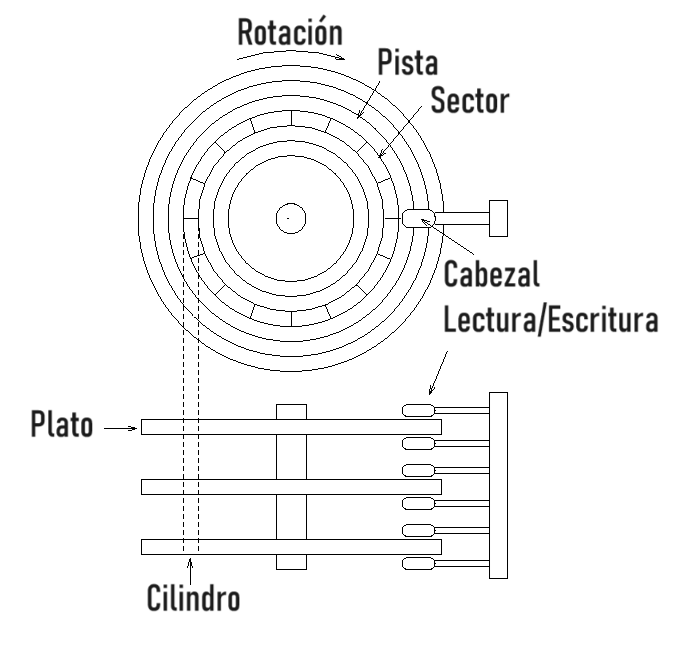
\includegraphics[width=0.75\linewidth]{figures/disk_platters.png}
    \caption{Estructura física de un disco mecánico}
    \label{fig:estructura_fisica_disco_mecanico}
\end{figure}

En el caso de los discos mecánicos, como podemos ver en la figura \ref{fig:estructura_fisica_disco_mecanico}, el controlador de disco utiliza ternas de números (número de cilindro, número de pista y número de sector) para gestionar la información del disco. Cada bloque de datos en el sistema de ficheros corresponde a varios sectores físicos del disco. La numeración de los sectores (bloques) sigue un criterio que favorece los accesos secuenciales \cite{Hdd}.\\

A nivel físico, se establece un factor de intercalación que permite resolver el problema de perder uno o varios sectores por efecto de la velocidad de rotación mientras estamos completando la transferencia interna de datos entre la controladora y el sistema operativo. Con ello, se reduce el número de rotaciones necesarias para leer, por ejemplo, una pista completa secuencialmente \cite{StorageSystems,valero2006}.\\

Por otro lado, en el caso de los discos de estado sólido, la organización física es diferente debido a la ausencia de partes móviles. En lugar de acceder a los datos a través de cilindros, pistas y sectores como en los discos duros mecánicos, en los discos de estado sólido los datos se almacenan y acceden de manera electrónica directamente en las celdas de memoria flash \cite{InsideSolidState}.

\subsection{Organización lógica de los datos en el disco}

Independientemente de la organización física que puedan presentar, la gran mayoría de los sistemas de ficheros de Unix siguen una estructura lógica fundamental para gestionar y acceder a los datos almacenados en el disco. Esta estructura lógica, presente en sistemas de ficheros tanto en discos duros mecánicos como en unidades de estado sólido, permite una gestión eficiente de los datos y una fácil navegación a través del sistema de ficheros \cite{valero2006, linuxstorage}.

\begin{figure}[h!]
    \centering
    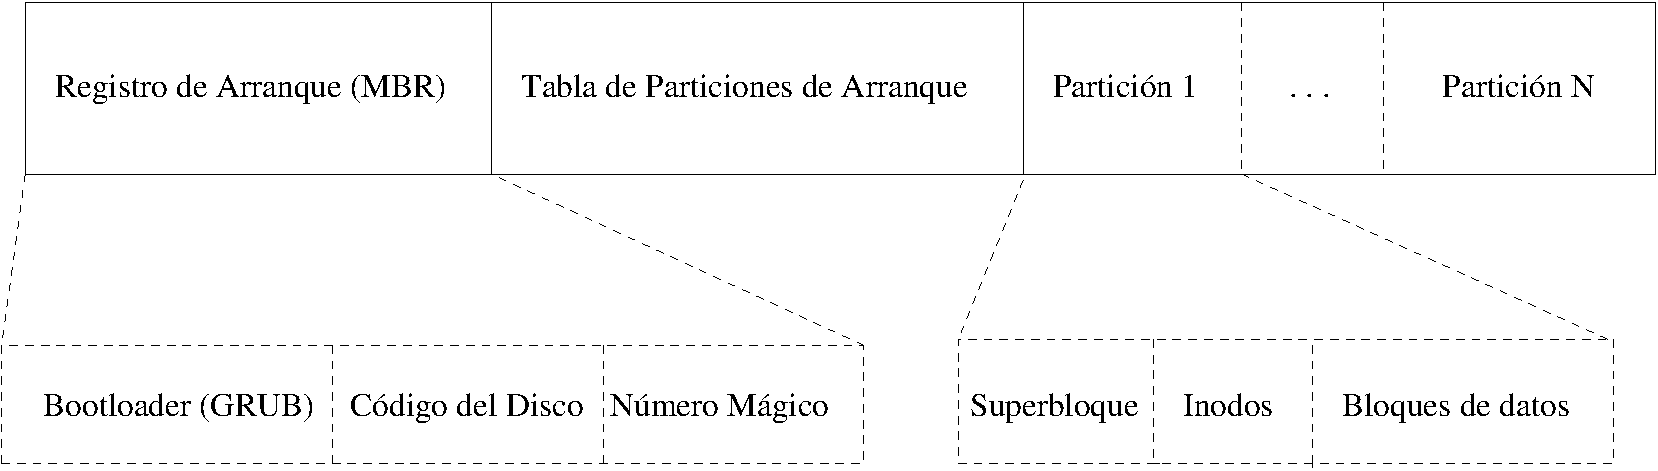
\includegraphics[width=1\linewidth]{figures/disk_logical_layout.pdf}
    \caption{Organización lógica de un disco}
    \label{fig:organizacion_logica_disco}
\end{figure}

En la figura \ref{fig:organizacion_logica_disco} se muestra la organización lógica de un disco en un sistema de ficheros tradicional, donde podemos observar las siguientes partes:

\subsubsection{MBR (master boot record)}

El MBR ocupa el primer sector o bloque del disco y contiene información esencial para el arranque del sistema y la gestión de las particiones del disco \cite{valero2006}.

\begin{itemize}
    \item \textbf{Bootloader:} El MBR almacena un programa de arranque, conocido como bootloader, que se encuentra en la primera etapa del proceso de arranque (bootstrap). El bootloader tiene la tarea de cargar el sistema operativo desde el disco y transferir el control al kernel del sistema operativo.
    
    \item \textbf{Código del disco:} Además del bootloader, el MBR puede contener código específico del disco que ayuda en el proceso de arranque, como rutinas de inicialización del hardware o controladores de dispositivo necesarios para acceder al disco y cargar el sistema operativo.
    
    \item \textbf{Número mágico:} El MBR finaliza con un número mágico de 2 bytes (0x55AA), conocido como firma de finalización, que indica que el MBR es válido y puede ser utilizado para arrancar el sistema. La presencia de esta firma es verificada por el firmware del sistema durante el proceso de arranque para determinar si el disco es arrancable. Este número mágico ha sido añadido recientemente para evitar ataques de tipo bootkit.
\end{itemize}

\subsubsection{Tabla de particiones de arranque}

La tabla de particiones de arranque, también conocida como la tabla de particiones MBR, se encuentra dentro del master boot record y describe cómo está dividido físicamente el disco en particiones. Actualmente, la tabla de particiones GPT (GUID Partition Table) es la más utilizada, ofreciendo mayor flexibilidad y soporte para discos de mayor tamaño.

\subsubsection{Particiones}

Las particiones son divisiones lógicas del disco y pueden contener diferentes sistemas de ficheros. En los sistemas de ficheros tipo Unix, cada partición suele presentar la estructura siguiente:
\begin{itemize}
    \item \textbf{Superbloque:} El superbloque es una estructura de datos crítica que se suele encontrar al inicio de un sistema de ficheros y contiene metadatos esenciales para el funcionamiento del mismo, como el tamaño total del sistema de ficheros, el tamaño de los bloques, el número de bloques libres, la ubicación de los inodos y la integridad de la partición. Es fundamental para el montaje y el mantenimiento del sistema.
    
    \item \textbf{Inodos:} Los inodos son estructuras de datos que contienen los atributos de los archivos, directorios y pipes del sistema de ficheros, cada uno de los cuales tiene asociado un inodo. Entre estos atributos se encuentra el identificador numérico del propietario (UID), del grupo de usuarios propietario (GID), máscara UGO de derechos, tamaño y ubicación en el conjunto de bloques de datos.
    
    \item \textbf{Bloques de datos:} En la parte final de la partición y ocupando la mayor parte de los bloques de la misma, se encuentran los bloques de datos, que contienen los bloques con el contenido de los ficheros, directorios y pipes. Los datos de los archivos se dividen en bloques de tamaño fijo o variable, y los inodos contienen punteros a estos bloques para acceder al contenido de los mismos.
\end{itemize}

\section{Sistema de ficheros en Linux: un análisis del sistema de ficheros virtual}

Entre otras cosas, el éxito de los sistemas Linux reside en su capacidad para interactuar sin inconvenientes con diversos sistemas de todo tipo. Esta capacidad se manifiesta en la posibilidad de montar discos o particiones que albergan formatos de fichero propios de sistemas como Windows, otros sistemas Unix e incluso sistemas como Amiga. Este destacado logro se sustenta en la implementación del innovador sistema de ficheros virtual (VFS). 

\subsubsection{El sistema de ficheros virtual}

El VFS constituye una pieza angular que opera como una capa de abstracción en el núcleo de Linux, gestionando todas las llamadas al sistema asociadas con el sistema de ficheros estándar de Unix. Su función principal consiste en proporcionar una interfaz unificada para distintos tipos de sistemas de ficheros.\\

Así, el sistema de ficheros virtual ofrece un amplio juego de llamadas al núcleo para la gestión de ficheros, las cuales son utilizadas para cualquiera de los tipos de sistemas de ficheros soportados por Linux. Cada una de estas llamadas tendrá en su implementación una parte común, es decir, ejecutada sea cual sea el sistema de ficheros subyacente, y una parte específica, que solo se ejecutará para el tipo concreto de sistema de ficheros con el que estemos trabajando en ese momento \cite{bovet2005,valero2006,bach1987}.

\subsubsection{Diversidad de sistemas de ficheros}

Los diferentes tipos de sistemas de ficheros soportados por el VFS pueden clasificarse en tres grandes grupos:

\begin{itemize}
    \item \textbf{Sistemas de ficheros basados en disco:} Son aquellos sistemas de ficheros que almacenan la información localmente en dispositivos de almacenamiento secundario (HDD, SSD, discos ópticos, memoria flash, etc).
    \item \textbf{Sistemas de ficheros en red:} Permiten el acceso a ficheros que se encuentran en otras computadoras en red. 
    \item \textbf{Sistemas de ficheros especiales:} Estos sistemas no gestionan espacio de almacenamiento real en disco, sino que actúan como interfaz con el sistema operativo para obtener o modificar información del mismo o de la configuración hardware. Un ejemplo es el sistema de ficheros \textit{/proc} en Linux.
\end{itemize}

El sistema de ficheros virtual introduce un modelo unificado para la gestión de archivos, lo que permite administrar todos los sistemas de ficheros compatibles. Por ejemplo, desde un sistema operativo Linux, un sistema de ficheros como NTFS (utilizado en Windows) se verá con una interfaz idéntica a la de Linux, incluyendo información sobre propietario, grupo y permisos UGO, adaptando las características específicas de cada sistema de ficheros al formato Unix de manera transparente \cite{love2010,tanenbaum2014}.

\section{Características principales de los sistemas de ficheros}\label{sec:caracteristicas_principales_sistemas_ficheros}

Después de examinar la organización de datos y comprender el funcionamiento del sistema de ficheros virtual, nos adentraremos en las características distintivas de los sistemas de ficheros de Linux. Exploraremos los elementos que los hacen únicos y los mecanismos implementados por el sistema para optimizar su rendimiento.

\subsection{Cachés del sistema} 

Los cachés, aunque son implementadas por el sistema operativo, desempeñan un papel crucial en los sistemas de ficheros y en las operaciones que estos realizan en el disco, así como en su rendimiento general. Por esta razón, es importante destacar los cachés más básicos que se encuentran en los sistemas actuales \cite{valero2006,bovet2005}.


\begin{figure}[!ht]
    \centering
    % TODO: falta la imagen original de esta figura en el repositorio
    % ("Screenshot 2024-02-06 at 23-12-08 ... .pdf.png"). Sustituir este
    % recuadro por \includegraphics cuando se recupere el archivo original.
    \fbox{\parbox[c][6cm][c]{0.70\linewidth}{\centering \itshape Figura no disponible: pendiente de recuperar la captura original}}
    \caption{Organización lógica del núcleo de Linux (VFS)}
    \label{fig:logica_organizacion_disco}
\end{figure}

Como se muestra en la figura \ref{fig:logica_organizacion_disco}, la interacción con los bloques del disco se realiza mediante el sistema de ficheros virtual. Este se encarga de traducir las solicitudes de lectura y escritura del sistema operativo en operaciones a nivel de bloques en el disco físico. El rendimiento y la eficiencia del sistema en estas operaciones está directamente influenciado por una serie de cachés que actúan como buffers para datos y metadatos frecuentemente utilizados. Estos cachés incluyen: 

\begin{itemize}
    \item \textbf{Caché de directorios:} Este caché contiene entradas de directorios recientemente utilizadas. Cuando se accede a un directorio, su contenido se almacena en el caché de directorios para agilizar futuros accesos. Este caché ayuda a reducir el tiempo de búsqueda de archivos en el sistema de ficheros al mantener en memoria las referencias a los directorios más utilizados. 
    
    \item \textbf{Caché de inodos:} El caché de inodos contiene los inodos en uso actualmente y posiblemente algunos usados recientemente. Los inodos son estructuras de datos que almacenan metadatos de archivos, como permisos, tamaño y ubicación en disco. Mantener una copia de los inodos en memoria facilita el acceso rápido a la información de los archivos y mejora el rendimiento del sistema de ficheros. 
    
    \item \textbf{Caché de páginas:} Este caché contiene las páginas desalojables de procesos, así como las páginas de archivos y directorios recientemente utilizadas. Cuando se accede a datos en el sistema de ficheros, las páginas correspondientes se almacenan en el caché de páginas para evitar lecturas repetidas desde el disco. Esto ayuda a reducir el tiempo de acceso a los datos y mejora el rendimiento general del sistema.
    
    \item \textbf{Buffer-cache:} El buffer-caché contiene los bloques de los dispositivos de bloques más recientemente utilizados. Cuando se leen o escriben datos en el sistema de ficheros, los bloques correspondientes se almacenan en el buffer-caché para minimizar las operaciones de lectura y escritura directamente en el disco. Esto ayuda a mejorar el rendimiento al reducir la latencia de acceso a los datos en el disco.
    
\end{itemize}

\subsection{Instantáneas en sistemas de ficheros de Linux} 
Las instantáneas, también conocidas como \textit{snapshots}, ofrecen una herramienta eficaz para capturar el estado de un sistema de ficheros en un momento específico, lo que facilita su restauración en caso de fallos o cambios no deseados. En el contexto de los sistemas de ficheros de Linux, existen dos tipos principales de instantáneas:

\begin{itemize}
    \item \textbf{Instantánea de imagen completa:}
    Captura el estado completo del sistema de ficheros, incluyendo todos los archivos, directorios, permisos y metadatos. Sin embargo, su creación puede ser extremadamente costosa en términos de recursos, tiempo y espacio de almacenamiento debido a la necesidad de duplicar todos los datos del sistema de ficheros. 
    
    \item \textbf{Instantánea de fichero o directorio específico:}
    Se enfoca en capturar el estado de un fichero o directorio específico en un momento determinado. Esta opción resulta ser menos exigente en términos de recursos y espacio de almacenamiento en comparación con la instantánea completa del sistema de ficheros.
\end{itemize}

Dado que este último tipo de instantánea es el implementado por la gran mayoría de sistemas de ficheros en el mercado, nos centraremos en describir su funcionamiento, el cual se representa en la figura \ref{fig:funcionamiento_snapshots}.

\begin{figure}[h!]
    \centering
    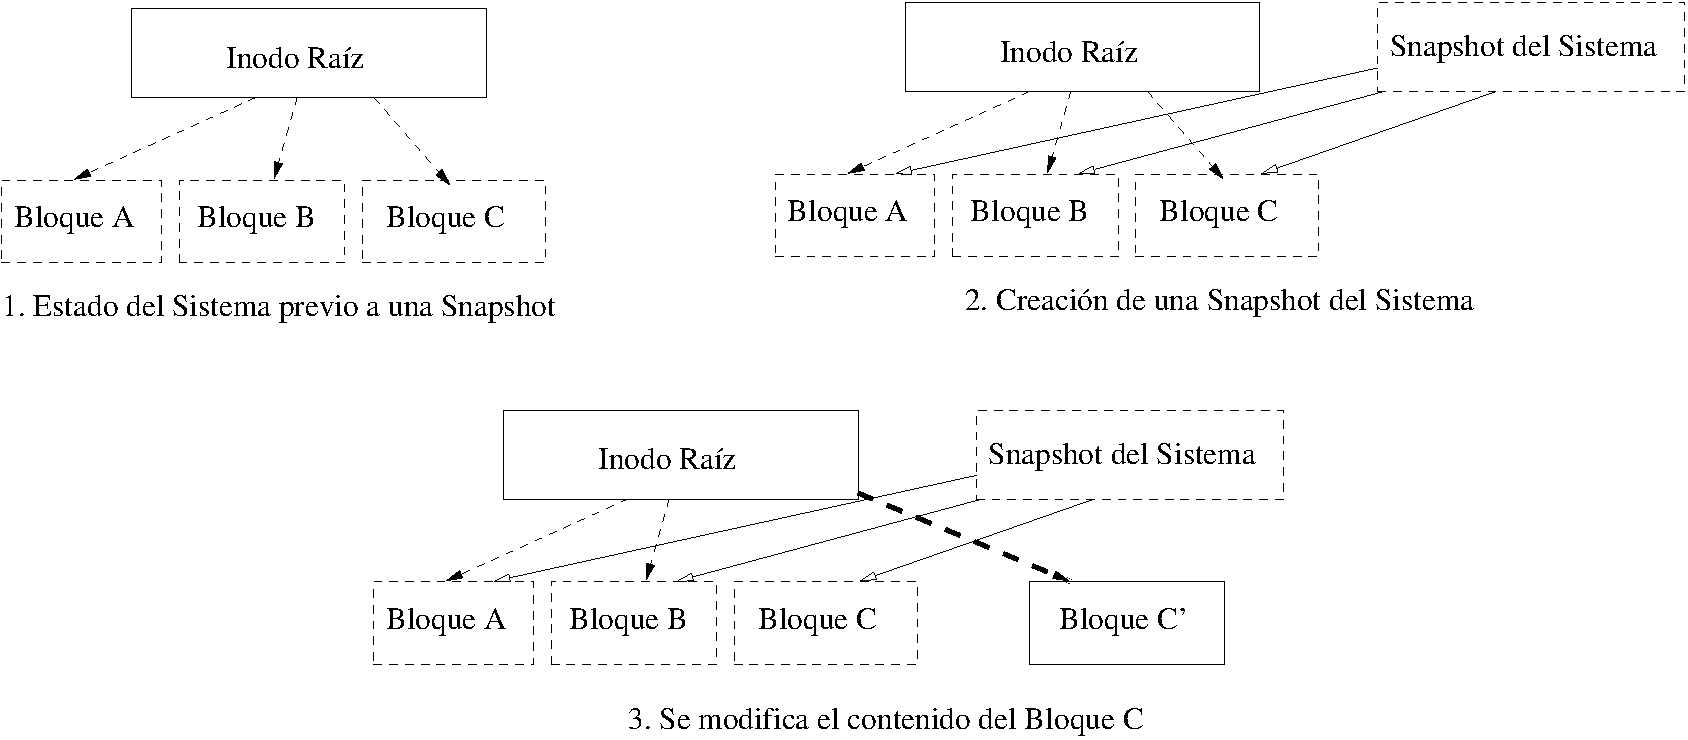
\includegraphics[width=1\linewidth]{figures/snapshots.pdf}
    \caption{Creación de una instantánea de un archivo}
    \label{fig:funcionamiento_snapshots}
\end{figure}

\begin{itemize}
    \item \textbf{Creación de la instantánea:}
        Partimos de un estado del sistema estable a partir del cual se crea la instantánea. Durante la creación de esta sobre un fichero, el sistema de ficheros captura el estado actual de los datos, generando una copia que refleja exactamente el contenido del mismo en ese instante, incluyendo todas las características de este, como su máscara UGO, propietario, entre otros.
    
    \item \textbf{Conservación de los datos originales:}
        Aunque el sistema puede continuar aceptando escrituras después de la creación de la instantánea, los datos originales permanecen intactos y accesibles a través de la misma. Es importante tener en cuenta que, aunque el sistema pueda seguir atendiendo peticiones de escritura después de crear una instantánea, la información salvaguardada en esta es una foto del estado del fichero o directorio en ese momento, pero su estado actual posiblemente habrá cambiado.
    
    \item \textbf{Restauración:}
        En situaciones de errores, pérdida de datos o cambios no deseados, es factible restaurar el fichero o directorio a un estado anterior utilizando la correspondiente instantánea. Esta restauración implica la vuelta del fichero o directorio a su estado capturado en el momento de la creación de la misma, incluyendo tanto su contenido como sus metadatos y configuraciones específicas.
        
\end{itemize}

Estas instantáneas se basan en la tecnología de copy on write (COW). A diferencia del COW utilizado para compartir memoria entre procesos diferentes, como por ejemplo a través de la llamada fork, esta implementación se emplea para compartir bloques de datos preexistentes al crear la instantánea. Solo se realiza una copia de los mismos cuando se modifican, optimizando así el proceso.

\subsection{Journaling en sistemas de ficheros de Linux}

El journaling, o registro de transacciones, es una técnica fundamental utilizada en los sistemas de ficheros para garantizar la integridad de los datos en caso de fallos del sistema o interrupciones inesperadas, como cortes de energía. Esta técnica consiste en mantener un registro detallado de las operaciones de escritura que se realizan en el sistema de ficheros antes de que se apliquen de manera definitiva \cite{bovet2005,linuxstorage}.

\begin{figure}[h!]
    \centering
    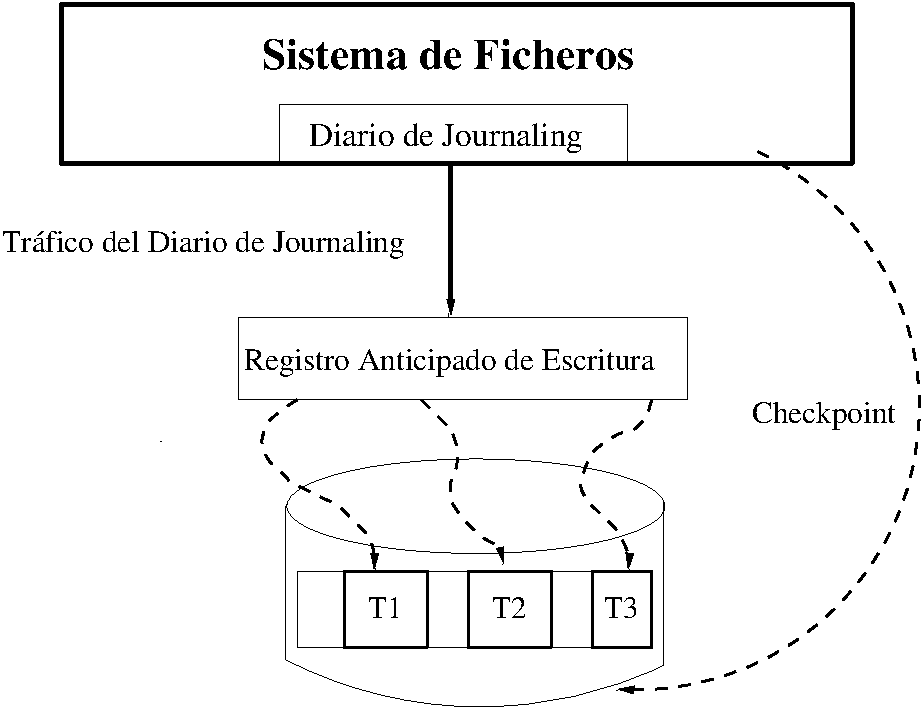
\includegraphics[width=0.55\linewidth]{figures/journaling.pdf}
    \caption{Ilustración del funcionamiento del journaling}
    \label{fig:funcionamiento_journaling}
\end{figure}

La gran mayoría de sistemas de ficheros dividen el proceso de journaling en tres pasos, que aparecen en la figura \ref{fig:funcionamiento_journaling} y se describen a continuación:

\begin{enumerate}
    \item \textbf{Registro inicial en el journal:} En esta etapa, se inicia el proceso creando una duplicación de los bloques destinados a ser escritos en el sistema de ficheros. Esta copia se almacena en el registro anticipado de escritura, y todos los datos registrados en esta fase quedan documentados en el diario de journaling del sistema de ficheros.

    \item \textbf{Confirmación en el journal:} Una vez que la transferencia de datos al registro anticipado de escritura se ha completado y los datos han sido confirmados en el diario de journaling, los bloques son finalmente escritos en el sistema de ficheros.

    \item \textbf{Finalización y confirmación en el sistema de ficheros:} En esta fase concluyente, después de finalizar la transferencia de datos al sistema de ficheros y confirmar la integridad en este último, se emite un checkpoint que valida el exitoso proceso de transferencia de datos. Posteriormente, las copias de los bloques almacenadas en el registro anticipado de escritura se descartan.
\end{enumerate}

El journaling también es beneficioso para minimizar la fragmentación y puede mejorar la eficiencia general del sistema de ficheros. Sin embargo, su objetivo principal es asegurar que las operaciones de escritura se completen de manera segura y coherente.

\subsection{Técnicas de gestión de los datos en discos: Trim y Defrag}

Dos técnicas clave sobresalen en la optimización del acceso a datos y el rendimiento eficiente: Trim y Defrag. Trim es esencial para maximizar tanto el rendimiento como la durabilidad de los dispositivos de estado sólido, siendo una técnica integrada en la gran mayoría de sistemas de ficheros actuales. Por otro lado, defrag se presenta como una técnica tradicional utilizada en discos duros magnéticos para organizar los datos y mejorar su accesibilidad, mediante la reorganización de los fragmentos de datos en el sistema de ficheros.

\subsubsection{Optimización de almacenamiento con Trim en SSD}

Trim es una técnica que capacita al sistema operativo para poder informar a una unidad de estado sólido basada en NAND flash acerca de los bloques de datos que ya no están en uso y pueden ser eliminados. Esta implementación no solo acelera la velocidad de escritura en los SSD, sino que también desempeña un papel clave en la prolongación de la vida útil de estos discos.\\

Cuando un fichero es eliminado de un SSD, el sistema operativo etiqueta esos bloques de memoria como "libres" para su posible sobreescritura. Sin embargo, en los SSD, la reescritura directa de bloques individuales, como en los discos duros magnéticos, no es posible. En cambio, los SSD deben borrar bloques completos antes de escribir nuevos datos. La función Trim mejora este proceso al enviar una señal al SSD, indicándole qué bloques de datos ya no están en uso. Esto permite que el SSD realice la "recolección de basura", donde los bloques marcados como no utilizados se borran y están listos para ser escritos nuevamente de manera más eficiente cuando sea necesario.

\subsubsection{Optimización de almacenamiento con Defrag en HDD}

La desfragmentación es una práctica esencial aplicada a los sistemas de ficheros modernos de discos duros magnéticos con el objetivo de reorganizar los fragmentos dispersos de datos en el disco. Este procedimiento tiene como finalidad mejorar el acceso a los archivos y, en última instancia, potenciar el rendimiento general del disco duro.\\

Es crucial resaltar que los discos duros magnéticos son especialmente susceptibles a la fragmentación debido a la naturaleza de su funcionamiento. En estos dispositivos, las pistas magnéticas en la superficie del disco almacenan información, y la cabeza de lectura/escritura debe desplazarse a lo largo de estas pistas para acceder a los datos.\\

Sin embargo, los SSD operan de manera completamente distinta, careciendo de cabezas de lectura/escritura móviles. En consecuencia, los SSD no experimentan los mismos problemas de fragmentación que los HDD y, por ende, no requieren procesos de desfragmentación tradicionales para mantener un rendimiento óptimo. La gestión de la fragmentación en los SSD está intrínsecamente integrada en su diseño y se aborda de manera más eficiente en comparación con los discos duros magnéticos.\\

Es importante destacar que la desfragmentación nunca ha sido una prioridad en los sistemas de ficheros de Linux, a diferencia de Windows, donde ha tenido una importancia significativa, especialmente en sistemas de ficheros como NTFS. En Windows, la desfragmentación se considera crucial para mantener el rendimiento del sistema. No obstante, en la actualidad, los sistemas de ficheros modernos de Linux, como ext4 y Btrfs, han comenzado a implementar técnicas de desfragmentación para mejorar la eficiencia del almacenamiento y el acceso a los datos. Estas mejoras reflejan un avance en la gestión del sistema de ficheros, adaptándose a las necesidades contemporáneas de los usuarios y a las capacidades de los dispositivos de almacenamiento modernos.

\subsection{Técnicas de gestión del espacio en disco: compresión y deduplicación}

Dos técnicas clave utilizadas por los sistemas de ficheros son la compresión y descompresión de archivos, así como la deduplicación. Estas estrategias juegan un papel vital en la eficiencia y la economía del almacenamiento digital, asegurando que aprovechemos al máximo nuestro espacio y recursos.

\subsubsection{Deduplicación de los datos}

La función de deduplicación se centra en eliminar duplicados exactos de datos, evitando la redundancia y mejorando la eficiencia en el almacenamiento. Generalmente los sistemas de ficheros abordan este proceso de la siguiente forma:

\begin{enumerate}
    \item \textbf{Identificación de datos duplicados:}
        El sistema de ficheros analiza constantemente los bloques de datos almacenados para identificar duplicados exactos. Esto puede aplicarse a nivel de ficheros completos o a bloques de datos más pequeños, según la implementación específica.
    
    \item \textbf{Creación de punteros compartidos:}
        En lugar de almacenar múltiples copias idénticas de un conjunto de datos, la deduplicación crea punteros compartidos que apuntan al mismo bloque de datos. Esto significa que, en la práctica, solo se guarda una copia de los datos duplicados, reduciendo el espacio necesario en disco.
    
    \item \textbf{Modos y configuración de deduplicación:}
        Algunos sistemas de ficheros permiten la deduplicación en tiempo real durante la escritura de datos. Otros también ofrecen opciones programadas, ejecutando el proceso en momentos específicos para minimizar el impacto en el rendimiento. Además, se puede configurar la deduplicación con políticas personalizadas, como la frecuencia de ejecución del proceso y las áreas particulares del sistema de ficheros que deben ser consideradas.
\end{enumerate}

La deduplicación de datos ofrece beneficios significativos en términos de ahorro de espacio en disco, especialmente en situaciones donde hay datos duplicados o redundantes. Sin embargo, es esencial considerar cuidadosamente la implementación y configuración de esta característica para maximizar sus beneficios sin comprometer el rendimiento del sistema.

\subsubsection{Compresión y descompresión de datos en sistemas de ficheros de Linux}

La compresión y descompresión de datos son procesos esenciales para optimizar el espacio en disco y mejorar la eficiencia en el almacenamiento. A continuación, al igual que con la deduplicación, detallaremos la implementación general que siguen los sistemas de ficheros para abordar esta técnica:

\begin{itemize}
    \item \textbf{Compresión en tiempo real:}
    Este enfoque implica la compresión de datos durante la escritura en el sistema de ficheros. Los datos son comprimidos antes de ser almacenados en el disco, lo que proporciona ahorros inmediatos en espacio. Sin embargo, puede haber un ligero impacto en el rendimiento durante la escritura debido al procesamiento adicional de compresión.
    
    \item \textbf{Compresión programada o por lotes:}
    En algunos casos, la compresión se programa para ejecutarse en momentos específicos o como un proceso por lotes. Esta estrategia permite realizar la compresión cuando la carga del sistema es menor, minimizando el impacto en el rendimiento. La compresión por lotes puede aplicarse a ficheros individuales o a directorios completos, empaquetando y comprimiendo la información según sea necesario. 
\end{itemize}

\subsection{Encriptación y seguridad en sistemas de ficheros}

La seguridad de los datos es una preocupación creciente en la era digital, especialmente en entornos donde la integridad y confidencialidad de la información son críticas. Los sistemas de ficheros EXT4, BTRFS, XFS y ZFS ofrecen diversas características de seguridad, incluyendo encriptación y mecanismos de protección avanzados que los hacen adecuados para entornos que manejan datos sensibles.

\subsubsection{Encriptación de datos}

La encriptación en el nivel de sistema de ficheros permite asegurar que los datos almacenados en disco sean inaccesibles sin las credenciales adecuadas. Mientras que EXT4 no cuenta con soporte nativo para encriptación, soluciones como eCryptfs y Fscrypt permiten añadir una capa de encriptación sobre este sistema de ficheros.\\

Por otro lado, BTRFS y ZFS integran capacidades de encriptación nativa que facilitan la gestión segura de los datos sin la necesidad de herramientas adicionales. ZFS ofrece encriptación nativa desde su versión 0.8, permitiendo la encriptación de datos y metadatos de manera transparente para el usuario. BTRFS también soporta encriptación a través de configuraciones específicas del kernel.

\subsubsection{Protección contra manipulaciones y corrupción de datos}

Además de la encriptación, la integridad de datos es otro pilar fundamental de la seguridad en sistemas de ficheros. ZFS destaca en este aspecto con su diseño que utiliza sumas de comprobación para todos los bloques de datos, lo que permite detectar y corregir errores automáticamente. BTRFS proporciona características similares con su enfoque en la redundancia y la capacidad de reparar datos corruptos utilizando copias almacenadas.\\

XFS y EXT4, mientras tanto, ofrecen opciones de journaling que mejoran la resistencia del sistema de ficheros frente a fallos del sistema, garantizando que las operaciones de ficheros se completen correctamente o se reviertan en caso de interrupción.

\subsection{Resumen de las características en los sistemas de ficheros a analizar}

\begin{table}[h!]
\centering
\caption{Comparación de características de los sistemas de ficheros EXT4, BTRFS, XFS y ZFS}
\label{tab:comparative-features}
\resizebox{\textwidth}{!}{%
\begin{tabular}{|l|c|c|c|c|}
\hline
\textbf{Característica} & \textbf{EXT4} & \textbf{BTRFS} & \textbf{XFS} & \textbf{ZFS} \\ \hline
Journaling & \checkmark & \checkmark & \checkmark & \checkmark \\ \hline
Snapshots & $\times$ & \checkmark & $\times$ & \checkmark \\ \hline
Deduplicación & $\times$ & \checkmark & $\times$ & \checkmark \\ \hline
Compresión & $\times$ & \checkmark & $\times$ & \checkmark \\ \hline
Integridad de datos & \checkmark & \checkmark & \checkmark & \checkmark \\ \hline
Cachés del sistema & \checkmark & \checkmark & \checkmark & \checkmark \\ \hline
Copy on Write (COW) & $\times$ & \checkmark & $\times$ & \checkmark \\ \hline
Tamaño de bloque & \texttt{1KiB-64KiB} & \texttt{4KiB-64KiB} & \texttt{512B-64KiB} & \texttt{4KiB-128KiB} \\ \hline
Tamaño nombre de archivo & \texttt{255 bytes} & \texttt{255 bytes} & \texttt{255 bytes} & \texttt{255 bytes} \\ \hline
Encriptación & \texttt{eCryptfs/Fscrypt} & \texttt{Kernel} & $\times$ & \checkmark \\ \hline
Protección de datos & \texttt{Journaling} & \texttt{Checksum} & \texttt{Journaling} & \texttt{Checksum} \\ \hline
TRIM Support & \checkmark & \checkmark & $\times$ & \checkmark \\ \hline
Defragmentación & \checkmark & $\times$ & \checkmark & $\times$ \\ \hline
\end{tabular}
}
\end{table}






% Chapter 3: File systems under study
\chapter{Sistemas de ficheros a analizar}\label{sec:capítulo_3}

\section{¿Por qué hemos elegido estos sistemas de ficheros?}

Medir el uso de los sistemas de ficheros es una tarea desafiante debido a la falta de estudios exhaustivos que recojan esta información de manera global. Ante esta dificultad, hemos optado por obtener el listado de las 64 distribuciones más descargadas en 2023 y analizar los sistemas de ficheros que soportan por defecto. La figura \ref{fig:uso sistemas de ficheros}, derivada de la tabla referenciada en el \nameref{sec:anexo}, nos proporciona una visión clara de la distribución del uso de sistemas de ficheros en estas distribuciones.

\begin{figure}[htbp]
    \centering
    \begin{tikzpicture}
        \begin{axis}[
            ybar,
            bar width=0.5cm,
            enlargelimits=0.15,
            ylabel={Número de distribuciones},
            xticklabels={EXT4, BTRFS, XFS, ZFS, Otros},
            xtick=data,
            nodes near coords,
            nodes near coords align={vertical},
            ymode=normal,
            ymin=10,
            ymax=60,
            x tick label style={rotate=45,anchor=east},
            ]
            \addplot coordinates {(0, 53) (1, 26) (2, 15) (3, 13) (4, 23)};
        \end{axis}
    \end{tikzpicture}
    \caption{Sistemas de ficheros más usados en 2023}
    \label{fig:uso sistemas de ficheros}
\end{figure}

Hemos seleccionado los sistemas de ficheros que estas distribuciones utilizan como predeterminados, entre los cuales se encuentran EXT4, BTRFS, XFS y ZFS. Estos sistemas no solo destacan por su amplio uso, sino también por su madurez y relevancia en el panorama actual de los sistemas de ficheros para Linux. Cada uno de ellos ofrece un conjunto único de características y funcionalidades que los hacen atractivos y confiables para diferentes aplicaciones y entornos de trabajo.

Entender la cronología de estos sistemas de ficheros es esencial para obtener una comprensión completa de su evolución y comprender cómo han llegado a ser lo que son en la actualidad. Con esta selección, no solo buscamos comprender las tendencias actuales en el uso de sistemas de ficheros en entornos Linux, sino también analizar detenidamente las características y capacidades de los sistemas más relevantes.

\begin{figure}[h!]
    \centering
    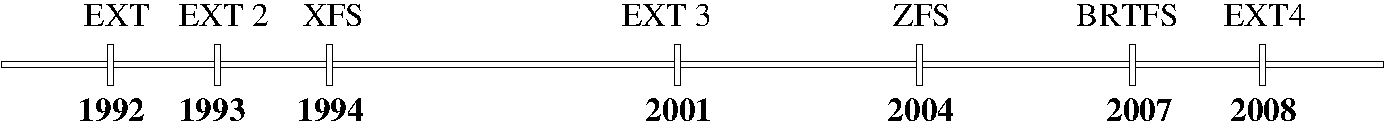
\includegraphics[width=1\linewidth]{figures/timeline.pdf}
    \caption{Línea de tiempo de los sistemas de ficheros de Linux}
    \label{fig:linea tiempo fs}
\end{figure}

El linaje de EXT4 se remonta a los primeros días del sistema de ficheros EXT, que apareció en 1992. Posteriormente, en 1993, se introdujo EXT2 como una mejora significativa, seguido por EXT3 en 2001, que ofrecía mejoras adicionales. Sin embargo, fue con la llegada de EXT4 en 2008, introducido en el kernel Linux 2.6.28, que el sistema de ficheros EXT alcanzó su punto más alto en términos de rendimiento, confiabilidad y capacidades avanzadas.

XFS, por otro lado, tiene sus raíces en los esfuerzos de Silicon Graphics Inc. (SGI) en 1994. Desarrollado como un sistema de ficheros de alto rendimiento para el sistema operativo IRIX, XFS se adaptó a Linux y se convirtió en una opción popular para aplicaciones que requieren un manejo eficiente de grandes volúmenes de datos. XFS se incorporó al kernel Linux en la versión 2.1.47, lanzada en 1997.

El surgimiento de BTRFS en 2007 marcó un hito en el desarrollo de sistemas de ficheros para Linux. Anunciado como un proyecto experimental, BTRFS fue concebido como un sistema de ficheros de próxima generación, que terminó siendo introducido en el kernel de Linux en la versión 2.6.29, lanzada en 2009.

ZFS, diseñado por Sun Microsystems en 2004, inicialmente para el sistema operativo Solaris, ha sido adoptado en entornos Linux mediante implementaciones de código abierto. Sin embargo, debido a diferencias de licencia entre la Licencia Pública General de GNU (GPL) utilizada por el kernel de Linux y la Licencia de Sun CDDL utilizada por ZFS, la integración oficial de ZFS en el kernel de Linux no se ha producido. En su lugar, existen proyectos de código abierto como OpenZFS que permiten utilizar ZFS en sistemas Linux.

\section{EXT4 (Extended File System 4)}

El sistema de ficheros EXT4 es uno de los sistemas de ficheros más utilizados en el entorno Linux debido a su robustez, eficiencia y capacidad para manejar grandes volúmenes de datos. Para comprender completamente cómo funciona EXT4, es crucial explorar su estructura interna y sus principales características.

\subsection{Estructura interna de EXT4}

\begin{figure}[h!]
    \centering
    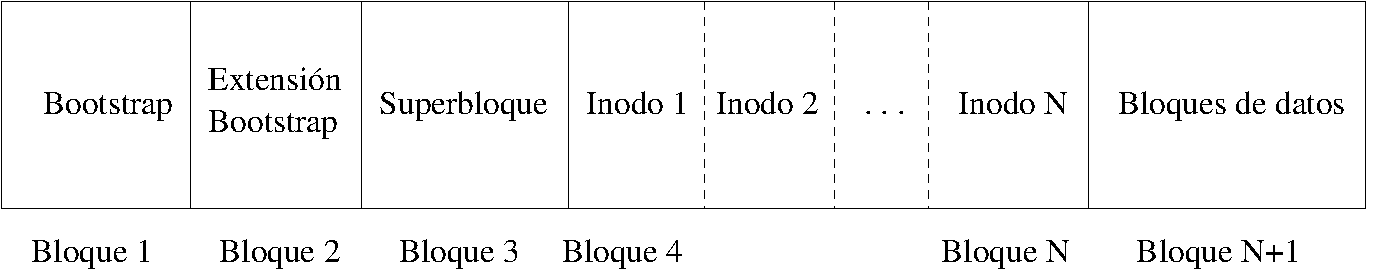
\includegraphics[width=0.85\linewidth]{figures/ext4.pdf}
    \caption{Estructura interna de EXT4}
    \label{fig:estructura interna de EXT4}
\end{figure}

La figura \ref{fig:estructura interna de EXT4} muestra la estructura interna del sistema de ficheros EXT4, que comparte la base de sus predecesores como EXT, EXT2 y EXT3 \cite{ext4-wiki,ext4_current_status,anatomy_ext4}. Esta estructura se compone de los siguientes elementos:

\begin{enumerate}
    \item \textbf{Arranque (Bootstrap):} El arranque se refiere al proceso inicial de carga del sistema operativo durante el inicio del sistema. En este proceso, se lleva a cabo la rutina de carga del kernel en memoria y una inicialización básica del hardware. Si no hay un cargador de arranque sofisticado como el GRUB, el kernel debe encontrarse en una posición fija en disco; de lo contrario, el cargador determina la partición y forma de arranque. Además, debe reconocer el formato del sistema de ficheros de arranque.

    \item \textbf{Extensión del Bootstrap:} Esta sección contiene datos adicionales necesarios para el arranque del sistema operativo, como la rutina llamada "setup" que termina la configuración del hardware. En EXT4, se incluyen mejoras en la eficiencia y rapidez de este proceso gracias a optimizaciones en la gestión de los metadatos y la estructura de almacenamiento.

    \item \textbf{Superbloque:} El superbloque es una estructura de metadatos que contiene información crucial sobre el sistema de ficheros EXT4. En este sistema de ficheros, el superbloque incluye elementos adicionales como referencias a los extents y timestamps necesarios para la optimización del acceso a los datos.
    
    \item \textbf{Lista de inodos:} Como ya hemos comentado previamente, los inodos son estructuras de datos que almacenan información sobre archivos, directorios y pipes en el sistema de ficheros. En EXT4, la lista de inodos secuencial permite un acceso más eficiente que sus antecesores.
    
    \item \textbf{Bloques de datos:} Los bloques de datos constituyen la parte principal del sistema de ficheros EXT4, ya que almacenan el contenido real de archivos, pipes y directorios. Estos bloques contienen una variedad de datos, incluyendo texto, imágenes gráficas en diferentes formatos, archivos binarios, entre otros.
\end{enumerate}

\subsection{Características de EXT4}

En cuanto a las características mencionadas anteriormente en la sección \ref{sec:caracteristicas_principales_sistemas_ficheros}, el sistema de ficheros EXT4 incluye características fundamentales como journaling, registrando las transacciones sobre el sistema de ficheros para garantizar la integridad de los datos en caso de fallos del sistema. Sin embargo, no ofrece soporte nativo para snapshots, \textit{copy on write}, compresión o deduplicación. En cambio, EXT4 cuenta con características que lo hacen único cómo son:

\textbf{Compatibilidad y retrocompatibilidad:} Fue diseñado específicamente para ser lo más compatible posible con EXT3, permitiendo la actualización in situ de sistemas de ficheros existentes previos como EXT3 y EXT2, así como el montaje automático de los mismos.\newline

\textbf{Grandes sistemas de ficheros:} EXT4 superó las limitaciones de direccionamiento de 32 bits de EXT3 mediante el uso de direccionamiento interno de 48 bits, permitiendo ficheros cuyo tamaño máximo es de 16 TiB, sobre un sistema de ficheros que en conjunto puede tener hasta 1 EiB.\newline

\textbf{Extents:} La implementación de extents simplifica la asignación y gestión de bloques físicos consecutivos, lo que resulta en una reducción del tamaño de la tabla de asignación. Aunque el espacio ocupado por el inodo permanece invariable, la adopción de bloques consecutivos simplifica las estructuras de almacenamiento necesarias para archivos grandes, reduciendo así el espacio requerido por estas tablas. Además de mitigar la fragmentación, esta mejora en la organización del almacenamiento también optimiza las operaciones de lectura.\newline

\textbf{Preasignación persistente:} Esta característica busca eliminar la necesidad de "blanquear" un bloque de datos con ceros cada vez que se asigna a un fichero, una operación comúnmente realizada para borrar su contenido anterior. En su lugar, el sistema hace uso de un "pool" de bloques previamente blanqueados, lo que agiliza la expansión de ficheros. En la práctica, esta mejora de rendimiento se evidencia en todas las situaciones, especialmente durante escrituras intensivas sobre el fichero.

\section{BTRFS (B-tree File System)}

BTRFS (B-tree File System) es un sistema de ficheros moderno, diseñado para ofrecer características avanzadas de gestión de almacenamiento de datos en entornos Linux. A diferencia de algunos sistemas de ficheros tradicionales, como EXT4, BTRFS utiliza una estructura de árbol B (B-tree) para organizar y gestionar los datos en el disco \cite{btrfs-docs,btrfs_design,btrfs_get_started,btrfs_swiss_army_knife}.

\begin{figure}[h!]
    \centering
    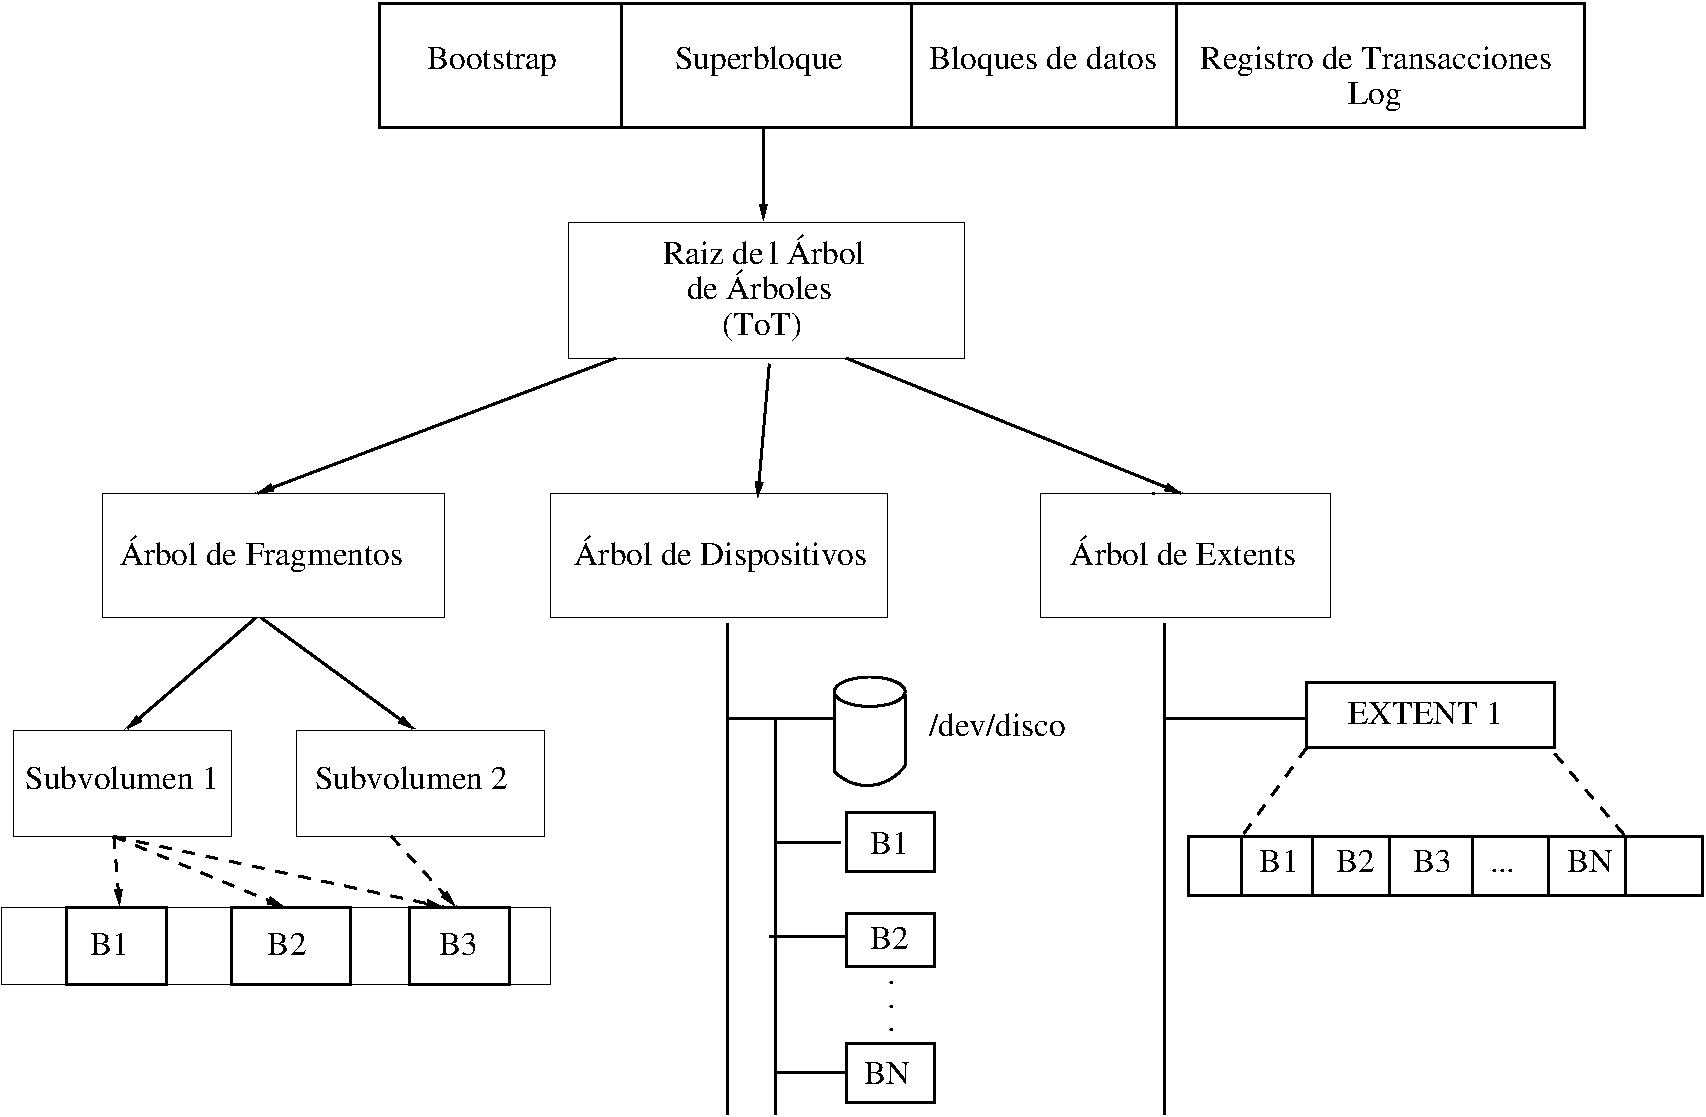
\includegraphics[width=1\linewidth]{figures/btrfs_btree.pdf}
    \caption{Estructura del superbloque en BTRFS}
    \label{fig:BTRFS-superblock}
\end{figure}

\subsection{Estructura interna de BTRFS}

Como podemos ver en la figura \ref{fig:BTRFS-superblock}, BTRFS presenta una estructura de sistema de ficheros más compleja en comparación con los sistemas EXT y sus extensiones, debido al uso que hace de árboles-B y funciones de hashing para almacenar la información.

En este contexto, el superbloque desempeña un papel fundamental al referenciar estructuras cruciales del disco. El superbloque contiene varias estructuras de datos que permiten organizar el almacenamiento de una forma muy eficiente, sobre todo de cara a acceder a la información. Estas estructuras de datos tienen una representación de árbol y son las siguientes:

\begin{itemize}
    \item \textbf{Raíz del árbol de árboles (TOT):} Es la raíz del árbol de metadatos en BTRFS. Contiene referencias a otros árboles importantes, como el árbol de fragmentos, el árbol de gestión de dispositivos y el árbol de almacenamiento por grupos de bloques. Es esencial para la navegación y la gestión del sistema de ficheros.
    
    \item \textbf{Árbol de fragmentos:} Este árbol organiza y gestiona los fragmentos de datos en el disco. Los fragmentos son bloques de datos físicos de tamaño fijo que se asignan dinámicamente para almacenar archivos y metadatos.
    
    \item \textbf{Árbol de gestión de dispositivos:} Este árbol nos permite conocer en qué dispositivos de almacenamiento tenemos representados los diferentes bloques de datos. Persigue una distribución eficiente del almacenamiento entre los dispositivos disponibles, gestionando cómo se asignan los bloques de datos a cada dispositivo.
    
    \item \textbf{Árbol de almacenamiento por grupos de bloques (extents):} Organiza los bloques de datos en grupos contiguos llamados "extents". Cada extent representa una región de bloques de datos consecutivos en el disco y se utiliza para asignar espacio a archivos y directorios en el sistema de ficheros BTRFS.
\end{itemize}

En BTRFS, es importante destacar que los inodos no se enumeran directamente después del superbloque, como suele ser el caso en otros sistemas de ficheros. En su lugar, se almacenan dentro del árbol de fragmentos. Esta implementación tiene la ventaja de agilizar la localización de los inodos mediante el uso de una estructura arborescente.

\subsection{Características de BTRFS}

BTRFS presenta características clave como \textit{copy on write}, snapshots y compresión y descompresión integradas, explicadas en la sección \ref{sec:caracteristicas_principales_sistemas_ficheros}. A continuación, resaltaremos algunas de las características específicas de BTRFS:

\textbf{Escritura retrasada:} La estrategia consiste en emplear la escritura diferida para agrupar un conjunto de escrituras consecutivas sobre un fichero en bloques posiblemente consecutivos, con el objetivo de reducir la fragmentación y mejorar el rendimiento. Esto se logra mediante el uso de los cachés de disco, que permiten acceder y utilizar esta información de forma rápida en la memoria principal antes de que se escriba en disco unos segundos más tarde. Para archivos pequeños, la escritura retrasada es especialmente ventajosa, ya que permite que múltiples operaciones de escritura pequeñas se acumulen en la caché antes de ser transferidas al disco.\newline

\textbf{Escritura coalescente:} Esta técnica de optimización se basa en agrupar múltiples operaciones de escritura pequeñas en una sola operación más grande antes de enviarlas al almacenamiento permanente. El objetivo es mejorar la eficiencia al reducir la cantidad de operaciones de E/S, disminuir la latencia y optimizar el uso de la caché del sistema. Las escrituras coalescentes son especialmente beneficiosas en operaciones secuenciales, donde las escrituras pueden ser combinadas de manera más efectiva, resultando en bloques de datos más grandes que se escriben de forma continua en el disco, mejorando así el rendimiento general del sistema.\newline

\textbf{Compartición de bloques:} La técnica de compartición de bloques permite que varios archivos compartan los mismos bloques de datos en el disco. El objetivo es optimizar el uso del espacio en disco y reducir la cantidad de escrituras necesarias. En lugar de escribir datos redundantes para cada archivo, los sistemas de archivos que emplean esta técnica pueden referenciar los mismos bloques de datos para diferentes archivos. Esto es especialmente útil para archivos pequeños y datos duplicados, ya que reduce la fragmentación y mejora la eficiencia del almacenamiento.\newline

\textbf{Gestión integrada de volúmenes:} BTRFS incorpora una gestión de volúmenes para facilitar la configuración y administración de almacenamiento, con soporte para RAID 0, RAID 1 y RAID 10, ofreciendo flexibilidad en la organización de dispositivos.\newline

\textbf{Auto-reparación y detección automática de inconsistencias:} BTRFS utiliza checksums para datos y metadatos, lo que permite la auto-reparación y detección automática de corrupciones. Estas corrupciones, que pueden ocurrir sin ser detectadas inicialmente, son verificadas y corregidas automáticamente gracias a los checksums, actuando como firmas digitales que garantizan la integridad de los datos.\newline

\textbf{Soporte para modo zonificado:} BTRFS es compatible con el modo zonificado, una técnica de asignación de bloques diseñada para adaptarse a dispositivos que implementan tecnologías como SMR (Shingled Magnetic Recording) y ZBC (Zoned Block Commands), utilizadas en discos magnéticos, así como ZNS (Zoned Namespace), específicamente diseñada para unidades de estado sólido. Estas tecnologías mejoran la eficiencia en la gestión de datos al organizarlos en zonas contiguas, facilitando la lectura secuencial y optimizando el rendimiento del almacenamiento.\cite{ZBC,ZNS}

\section{XFS (X File System)}

XFS, o Extents File System, es un sistema de ficheros de alto rendimiento utilizado como predeterminado en la familia Red Hat Enterprise Linux (RHEL), una distribución de Linux desarrollada por Red Hat \cite{xfs-wiki,weil2006ceph,sweeney1996scalability,beck1997xfs,soltis2007xfs}. A lo largo de su desarrollo, XFS ha pasado por varias generaciones, dando lugar a tres versiones distintas de este sistema de ficheros:

\begin{itemize}
    \item \textbf{Primera generación (XFS simple):} Diseñada para el sistema operativo IRIX, basado en UNIX y desarrollado por Silicon Graphics, Inc. (SGI). IRIX fue el sistema operativo principal utilizado en las máquinas SGI.
    
    \item \textbf{Segunda generación (Origen de las primeras versiones del sistema de ficheros):} Utilizado principalmente en dispositivos de Almacenamiento Conectado a la Red (NAS).

    \item \textbf{Tercera generación XFS de Linux - generación 3:} La versión más reciente, implementada en sistemas modernos basados en Linux. Introduce cambios significativos en el formato de los metadatos para mejorar su identificación y verificación y presenta la organización mostrada en la figura \ref{fig:organización lógica XFS}.
\end{itemize}

\subsection{Estructura interna de XFS}

Como vemos en la figura \ref{fig:organización lógica XFS}, XFS organiza el almacenamiento en grupos de asignación, también conocidos como AG (por sus siglas en inglés, Allocation Groups). Cada grupo de asignación contiene una porción del espacio de almacenamiento del sistema de ficheros y se encarga de administrar sus propios recursos, como inodos y bloques de datos \cite{brand2012assuring,pate2004unix,card1996xfs}. Dentro de cada grupo tenemos una estructura con la información siguiente:

\begin{figure}[h!]
    \centering
    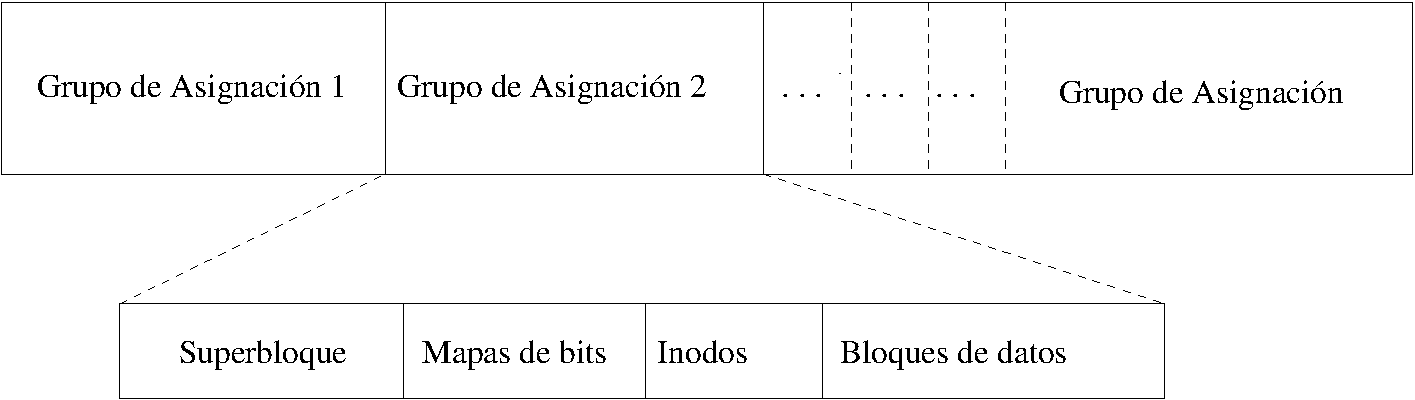
\includegraphics[width=1\linewidth]{figures/xfs.pdf}
    \caption{Organización lógica de XFS}
    \label{fig:organización lógica XFS}
\end{figure}

\begin{itemize}
    \item \textbf{Mapas de bits:} XFS utiliza mapas de bits para gestionar el estado de cada bloque en el grupo de asignación, lo que permite una gestión precisa y eficaz del espacio de almacenamiento.

    \item \textbf{Inodos:} En XFS, al igual que en los demás sistemas de ficheros analizados, los inodos representan archivos, directorios y pipes, almacenando información vital como permisos, propietarios, tamaño y ubicación de los datos del archivo. Sin embargo, los inodos en XFS tienen características especiales que los distinguen. En particular, XFS utiliza inodos extendidos, los cuales pueden almacenar atributos adicionales y extensiones de metadatos. Además, XFS implementa un esquema avanzado de asignación dinámica de inodos, contribuyendo a un rendimiento superior en operaciones de E/S y una mayor escalabilidad del sistema de ficheros.

    \item \textbf{Bloques de datos:} Los bloques de datos en XFS contienen los datos reales de los archivos y directorios, y pueden organizarse de diversas formas según las necesidades del sistema de ficheros. Esta flexibilidad en la organización de bloques de datos permite una adaptación óptima a diferentes cargas de trabajo y requisitos de almacenamiento.
\end{itemize}

\subsection{Características de XFS}

En cuanto a las características mencionadas anteriormente en la sección \ref{sec:caracteristicas_principales_sistemas_ficheros}, el sistema de ficheros XFS, al igual que EXT4 y BTRFS, ofrece una amplia gama de capacidades avanzadas. Entre estas características se incluyen el journaling para garantizar la integridad de los datos en caso de fallos del sistema. Sin embargo, no ofrece soporte nativo para snapshots, \textit{copy on write}, compresión o deduplicación. En cambio, ofrece las siguientes características:

\textbf{Administrador de Volúmenes XLV (Volume Manager XLV):} En el sistema de ficheros XFS, el administrador de volúmenes XLV proporciona una capa de abstracción adicional entre el sistema de ficheros y los dispositivos de almacenamiento físico. Pudiendo implementar configuraciones como \textit{striping}, \textit{mirroring} y \textit{concatenación} \cite{soltis2007xfs}.

El \textit{striping} distribuye equitativamente los datos entre varios discos, mejorando el rendimiento al permitir la lectura y escritura simultánea en múltiples dispositivos, especialmente en entornos de alta demanda. El \textit{mirroring} duplica la información en múltiples discos para aumentar la tolerancia a fallos y garantizar la integridad de los datos en XFS. Por otro lado, la \textit{concatenación} combina varios discos en un solo volumen lógico, facilitando la gestión eficiente de grandes cantidades de datos.

\textbf{Soporte para ACL y atributos extendidos:} XFS admite listas de control de acceso (ACL) y atributos extendidos, proporcionando una mayor funcionalidad en comparación con los permisos básicos de la máscara UGO. Estas características permiten una gestión más detallada de los permisos de acceso, así como el almacenamiento de información adicional asociada con los archivos y directorios, ofreciendo un control más preciso y enriquecido sobre la seguridad y los metadatos.

\textbf{Optimización para acceso paralelo:} Una de las características distintivas de XFS es su habilidad para dividir el espacio de almacenamiento en grupos de asignación independientes. Esta funcionalidad crea un entorno propicio para realizar operaciones de entrada/salida (E/S) de manera simultánea y eficiente. No solo acelera de manera significativa el rendimiento del sistema de ficheros, sino que también permite la ejecución paralela de múltiples operaciones de lectura y escritura, mejorando así la eficacia y capacidad de respuesta del sistema.

\section{ZFS (Zettabyte File System)}

ZFS es un sistema de ficheros transaccional diseñado para garantizar la integridad de los datos en todo momento. A diferencia de los sistemas de ficheros tradicionales que sobrescriben datos in situ y pueden dejar el sistema en un estado incoherente en caso de fallos, ZFS utiliza un enfoque transaccional completo. Lo que asegura que el estado del sistema de ficheros siempre sea coherente en disco.

\subsection{Estructura interna de ZFS}

La funcionalidad y organización del sistema de ficheros ZFS se presentan detalladamente en la figura \ref{fig:estructura ZFS}. Este diagrama proporciona una visión completa de cómo se relacionan los discos con los distintos elementos de abstracción específicos de ZFS. 

\begin{figure}[h!]
    \centering
    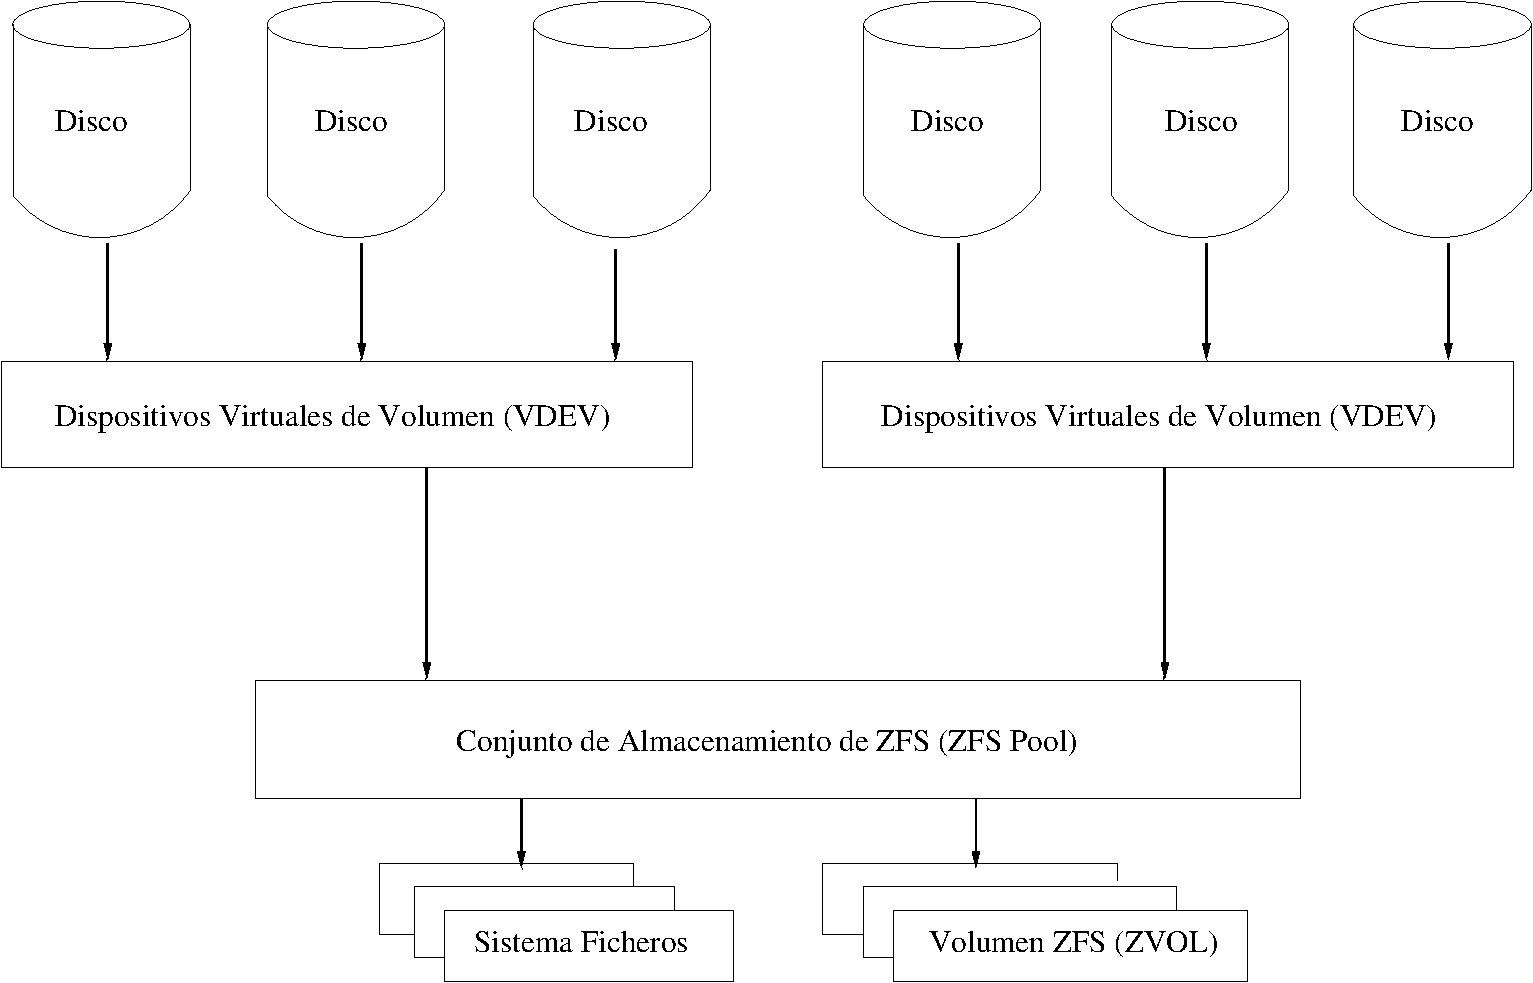
\includegraphics[width=1\linewidth]{figures/zfs.pdf}
    \caption{Organización del sistema de ficheros ZFS}
    \label{fig:estructura ZFS}
\end{figure}

\begin{itemize}
    \item \textbf{Zpool:} La unidad de almacenamiento de más alto nivel en ZFS. Un zpool puede consistir en uno o varios dispositivos de almacenamiento físicos como discos duros o SSDs, incluyendo configuraciones sobre dispositivos de almacenamiento en red.
    \item \textbf{Vdevs (Virtual Devices):} Los Vdevs son los bloques constructivos de un zpool, proporcionando la capacidad de agrupar dispositivos físicos para mejorar la redundancia y el rendimiento.
    \item \textbf{Datasets:} Conjuntos de datos que contienen información y metadatos, que pueden ser sistemas de archivos, volúmenes o instantáneas. Los datasets heredan propiedades del zpool pero también pueden tener configuraciones específicas como límites de espacio, compresión y deduplicación.
    \item \textbf{Zvols (ZFS Volumes):} Volumen de almacenamiento que simula un dispositivo de bloque, permitiendo el uso de aplicaciones que necesitan un sistema de ficheros convencional.
\end{itemize}

\subsection{Características de ZFS}

\textbf{Gestión de volúmenes integrada:} ZFS simplifica la gestión de volúmenes al combinar funciones de sistema de ficheros y administración de volúmenes en un único conjunto de herramientas. Soporta configuraciones RAID-Z, que ofrecen redundancia y tolerancia a fallos similar a RAID, pero con características avanzadas.\newline
    
\textbf{Integridad de datos con checksums:} ZFS garantiza la integridad de los datos mediante el uso de checksums. Cada bloque de datos contiene un checksum que se verifica durante las operaciones de lectura, facilitando la detección y corrección de errores silenciosos en los datos almacenados.\newline
    
\textbf{Conciencia de SSD/NVMe:} ZFS es consciente de las características de las tecnologías SSD/NVMe, aprovechando el soporte de TRIM/Discard, detalladas en la sección \ref{sec:caracteristicas_principales_sistemas_ficheros}. Esto optimiza las operaciones de almacenamiento, mejora el rendimiento general y contribuye a prolongar la vida útil de los dispositivos de almacenamiento flash.\newline
    
\textbf{Algoritmos de reparación automática:} En configuraciones RAID-Z, ZFS utiliza información de paridad para realizar reparaciones automáticas de datos corruptos, mejorando la fiabilidad del sistema de ficheros y protegiendo contra pérdidas de datos.\newline

\textbf{Soporte para modo zonificado:} ZFS es compatible con el modo zonificado, al igual que con BTRFS, se trata de una técnica de asignación de bloques adaptada a dispositivos de almacenamiento SMR/ZBC/ZNS. Esto mejora la eficiencia en la gestión de datos en entornos de almacenamiento zonificado.







% Chapter 4: Methodology
\chapter{Enfoque y metodología}\label{sec:capítulo_4}

Este capítulo describe el enfoque metodológico adoptado para comparar los sistemas de archivos ext4, Btrfs, XFS y ZFS bajo sus configuraciones predeterminadas. Se diseñó una batería de pruebas para evaluar la capacidad de estos sistemas para manejar operaciones básicas de entrada/salida, como lectura y escritura, así como pruebas especializadas, como la lectura estratificada y la lectura hacia atrás, para examinar el comportamiento bajo condiciones más exigentes.\\

Debido a las limitaciones de tiempo y recursos de un trabajo de fin de grado, se seleccionó Iozone como la herramienta principal para la evaluación del rendimiento. Esta elección se justifica por la practicidad y eficacia de Iozone, así como su amplia utilización en investigaciones sobre el rendimiento de los sistemas de archivos. La robustez de Iozone está documentada en estudios de investigadores destacados como Jan Kara \cite{kara2010btrfs} y Dominique A. Heger \cite{heger2012fs}. La relevancia de estos trabajos y su relación con la presente investigación se discuten en detalle en la sección de \hyperref[sec:trabajos relacionados]{Trabajos relacionados}, proporcionando un marco teórico que respalda las metodologías utilizadas.\\

La integración de pruebas estándar y especializadas permitirá una evaluación comprensiva de cada sistema de archivos, asegurando que los resultados sean representativos de sus capacidades en escenarios de uso real y controlados.

\section{Selección de la herramienta de evaluación}

La elección de la herramienta adecuada para evaluar el rendimiento de los sistemas de archivos es crucial. Las herramientas disponibles se dividen en dos categorías principales: aplicaciones de uso real y herramientas de evaluación sintéticas. Mientras que las aplicaciones reales pueden ofrecer una visión precisa del rendimiento en contextos específicos, encontrar una aplicación perfectamente representativa y adaptable a todas las configuraciones de sistema es complejo y consume mucho tiempo. Las herramientas sintéticas, aunque no simulan directamente cargas de trabajo reales, permiten evaluar el rendimiento bajo una variedad controlada de condiciones mediante la manipulación de parámetros de prueba.\\

Iozone, una herramienta sintética, se seleccionó debido a su capacidad para ajustar detalladamente el tamaño del archivo y el patrón de acceso, lo que permite medir el rendimiento de lectura y escritura de manera exhaustiva y flexible. Esta herramienta es eficiente para generar y medir una serie de operaciones de archivo bajo demanda, posibilitando la evaluación sistemática de cada sistema de archivos en condiciones idénticas y repetibles. Además, Iozone ha sido ampliamente validada en la comunidad científica y técnica, como lo demuestran estudios previos incluidos en la sección \hyperref[sec:trabajos relacionados]{Trabajos relacionados}.

\subsection{Descripción y uso de Iozone}

Iozone es una herramienta ampliamente reconocida por su capacidad para adaptar exhaustivamente las pruebas de rendimiento a las necesidades específicas de cualquier sistema de archivos. Utiliza una variedad de operaciones de prueba para medir el rendimiento de E/S, incluyendo lectura, escritura, relectura, reescritura y operaciones especializadas como mmap y acceso de E/S asíncrono.\\

\begin{tcolorbox}[title=Código de ejemplo para Iozone, fonttitle=\bfseries, colback=gray!5!white, colframe=gray!75!black]
\begin{footnotesize}
\begin{verbatim}
# Comando para una prueba exhaustiva con Iozone
iozone -Raz -i0 -i1 -i2 -i3 -i4 -i5 -i8 -g32G -f /mnt/testfile -b ext4_00.xls
64 128 256 512 1024 2048 4096 8192 16384

8192  3737270 3688723 3782110 3653812 3229054 2394606 1893744 1762507
16384 3766316 3794181 3806792 3738857 3192571 2393255 1849445 1667268
32768 3807088 3844682 3856008 3782986 3264443 2373819 1816514 1622085
65536 3864617 3895838 3901866 3825782 3303391 2385889 1815048 1605015
\end{verbatim}
\end{footnotesize}
\end{tcolorbox}

El comando anterior muestra un ejemplo de cómo se puede configurar Iozone para realizar una prueba exhaustiva. Aquí hay una descripción de los parámetros utilizados:
\begin{itemize}
    \item \texttt{-R}: Genera un informe en formato Excel.
    \item \texttt{-a}: Realiza todas las operaciones de prueba disponibles.
    \item \texttt{-z}: Activa las pruebas para todos los tamaños de registro.
    \item \texttt{-i0 -i1 -i2 -i3 -i4 -i5 -i8}: Realiza pruebas de lectura, escritura, relectura, reescritura, lectura aleatoria, escritura aleatoria y lectura estratificada.
    \item \texttt{-g32G}: Establece el tamaño del conjunto de datos para la prueba en 32 GB.
    \item \texttt{-f /mnt/testfile}: Especifica el archivo de prueba a usar.
    \item \texttt{-b ext4\_00.xls}: Especifica el nombre del archivo de salida donde se guardarán los resultados de la prueba en formato Excel.
\end{itemize}

Los números en la parte inferior del código representan el tamaño del bloque de registro (en kbytes) y el rendimiento de E/S (en Kbytes/sec) para cada tamaño de bloque de registro.\\

\subsection{Configuración de prueba de Iozone}

Las pruebas de rendimiento de Iozone se llevarán a cabo utilizando una amplia gama de tamaños de bloque y fichero para evaluar exhaustivamente el rendimiento de los sistemas de archivos en diferentes condiciones.

\begin{tcolorbox}[title=Tamaños de bloque utilizados, colback=blue!5!white, colframe=gray!75!black]
Los tamaños de bloque son fundamentales para medir el rendimiento de E/S. Iozone ejecutará las operaciones de prueba utilizando los siguientes tamaños de bloque:
\begin{itemize}
    \item \textbf{Pequeños}: 4, 8, 16, 32, 64, 128 KB
    \item \textbf{Medianos}: 256, 512 KB, 1, 2 MB
    \item \textbf{Grandes}: 4, 8, 16 MB
\end{itemize}
\end{tcolorbox}

\begin{tcolorbox}[title=Tamaños de fichero utilizados, colback=blue!5!white, colframe=gray!75!black]
Los tamaños de fichero son otro aspecto importante a considerar. Iozone realizará pruebas con los siguientes tamaños de fichero:
\begin{itemize}
    \item \textbf{Pequeños}: 64, 128, 256, 512 KB, 1, 2, 4 MB
    \item \textbf{Medianos}: 8, 16, 32, 64, 128 MB
    \item \textbf{Grandes}: 256, 512 MB, 1, 2, 4, 8, 16, 32 GB  
\end{itemize}
\end{tcolorbox}

Estos tamaños de bloque y fichero han sido seleccionados para abarcar una amplia variedad de escenarios de uso y proporcionar una evaluación exhaustiva del rendimiento de los sistemas de archivos bajo diferentes condiciones de carga. Cada combinación de tamaño de bloque y fichero permitirá obtener información detallada sobre cómo se comportan los sistemas de archivos en diversas situaciones.

\section{Entorno de evaluación y repetición del experimento}

El estado del sistema durante el proceso de evaluación puede tener un impacto significativo en los resultados obtenidos. Para garantizar condiciones de prueba estables y consistentes, se implementan varias medidas de control y optimización.

\subsection{Control del estado del sistema}

Se llevan a cabo las siguientes acciones para controlar y estabilizar el estado del sistema durante las pruebas:
\begin{itemize}
    \item \textbf{Apagado de procesos no esenciales:} Se detienen todos los procesos no esenciales que podrían afectar las mediciones de rendimiento, garantizando así que los recursos del sistema estén dedicados exclusivamente a las pruebas.
    \item \textbf{Reinicio para pruebas de lectura/escritura:} Para las pruebas de lectura y escritura de archivos y directorios, se reinicia el sistema para eliminar cualquier influencia residual de pruebas anteriores y garantizar la coherencia de los resultados.
\end{itemize}

\subsection{Configuración de la partición}

Para cada sistema de archivos bajo evaluación, se crea una partición dedicada que ocupa todo el disco disponible utilizando una tabla de particiones GPT. Esta configuración garantiza que cada sistema tenga acceso al máximo espacio disponible y ayuda a prevenir la fragmentación del disco, lo que podría afectar negativamente el rendimiento del sistema de archivos. Después de cada prueba, se borra y se crea una nueva partición para asegurar condiciones consistentes.

\subsubsection{Crear la tabla de particiones}

Para crear la tabla de particiones GPT y una partición usando \texttt{gdisk}, se siguen los siguientes pasos:

\begin{tcolorbox}[title=Comandos para crear la tabla de particiones GPT]
\begin{verbatim}
# Crear tabla de particiones GPT y partición usando gdisk
sudo gdisk /dev/sdX
o   # Crear nueva tabla de particiones GPT
n   # Crear nueva partición (todo el disco)
w   # Escribir cambios y salir
\end{verbatim}
\end{tcolorbox}

\subsubsection{Crear particiones de sistemas de archivos individuales}
Para crear las particiones individuales se siguen los siguientes pasos:

\begin{tcolorbox}[title=Comandos para ext4]
\begin{verbatim}
# Crear el sistema de archivos ext4
sudo mkfs.ext4 /dev/sdX1

# Montar la partición
sudo mount /dev/sdX1 /mnt/ext4_test
\end{verbatim}
\end{tcolorbox}

\begin{tcolorbox}[title=Comandos para Btrfs]
\begin{verbatim}
# Crear el sistema de archivos Btrfs
sudo mkfs.btrfs /dev/sdX1

# Montar la partición
sudo mount /dev/sdX1 /mnt/btrfs_test
\end{verbatim}
\end{tcolorbox}

\begin{tcolorbox}[title=Comandos para XFS]
\begin{verbatim}
# Crear el sistema de archivos XFS
sudo mkfs.xfs /dev/sdX1

# Montar la partición
sudo mount /dev/sdX1 /mnt/xfs_test
\end{verbatim}
\end{tcolorbox}

\begin{tcolorbox}[title=Comandos para ZFS]
\begin{verbatim}
# Instalar ZFS en Arch Linux
sudo pacman -S zfs-linux

# Cargar el módulo ZFS
sudo modprobe zfs

# Crear un pool ZFS
sudo zpool create zfs_pool /dev/sdX

# Crear un sistema de archivos ZFS
sudo zfs create zfs_pool/zfs_test

# Montar el sistema de archivos ZFS 
sudo mount -t zfs zfs_pool/zfs_test /mnt/zfs_test
\end{verbatim}
\end{tcolorbox}

\subsection{Repetición del experimento}

Para asegurar la validez y fiabilidad de los resultados, cada prueba se repetirá 10 veces para cada sistema de archivos evaluado. Se calcularán las medias y desviaciones típicas de los resultados obtenidos para mitigar las variaciones aleatorias y garantizar mediciones precisas. Entre cada repetición, el equipo se apagará y se reiniciará para eliminar cualquier efecto residual y mantener un entorno de prueba consistente.\\

Este enfoque metodológico riguroso asegura la coherencia y confiabilidad de los resultados, permitiendo una evaluación precisa del rendimiento de los sistemas de archivos en diversas condiciones y cargas de trabajo.



% Chapter 5: Detailed results
\chapter{Resultados detallados}

Este capítulo presenta una evaluación exhaustiva del rendimiento de los sistemas de ficheros ext4, Btrfs, XFS y ZFS bajo una serie de condiciones de prueba específicas. 

\section{Pruebas de lectura}

\subsection{Lectura}

En la prueba de lectura secuencial, podemos apreciar cómo Btrfs obtiene un rendimiento excelente para tamaños de fichero muy pequeños, entre 4 kB y 65 kB, incluso cuadruplicando el rendimiento de los demás sistemas de ficheros comparados. Este comportamiento se fundamenta en su estructura arborescente, así como en la subasignación de bloques. Btrfs implementa una subasignación de bloques que permite manejar eficientemente archivos pequeños. En Btrfs, los bloques se pueden dividir en sub-bloques más pequeños, y múltiples archivos pequeños pueden ocupar diferentes sub-bloques dentro del mismo bloque. Esto reduce el espacio desperdiciado y permite que el sistema de ficheros mantenga una alta densidad de datos. Como resultado, cuando el sistema necesita acceder a un archivo pequeño, puede localizarlo y cargarlo rápidamente desde el bloque contiguo, mejorando el rendimiento.\\

También apreciamos cómo en Btrfs, puesto que el tamaño de bloque elegido para la prueba es de 8 kB, el rendimiento de este sistema de ficheros aumenta hasta llegar a 8 kB de tamaño de fichero. Esto se debe a la lectura multisector, que se refiere a la capacidad del sistema de leer múltiples sectores consecutivos del disco en una sola operación. Esta aceleración producida por la lectura multisector se va perdiendo una vez superado el tamaño de bloque, lo que se puede ver reflejado a partir de los 8 kB de tamaño de fichero. \\

\newpage

\begin{figure}[h!]
    \centering
    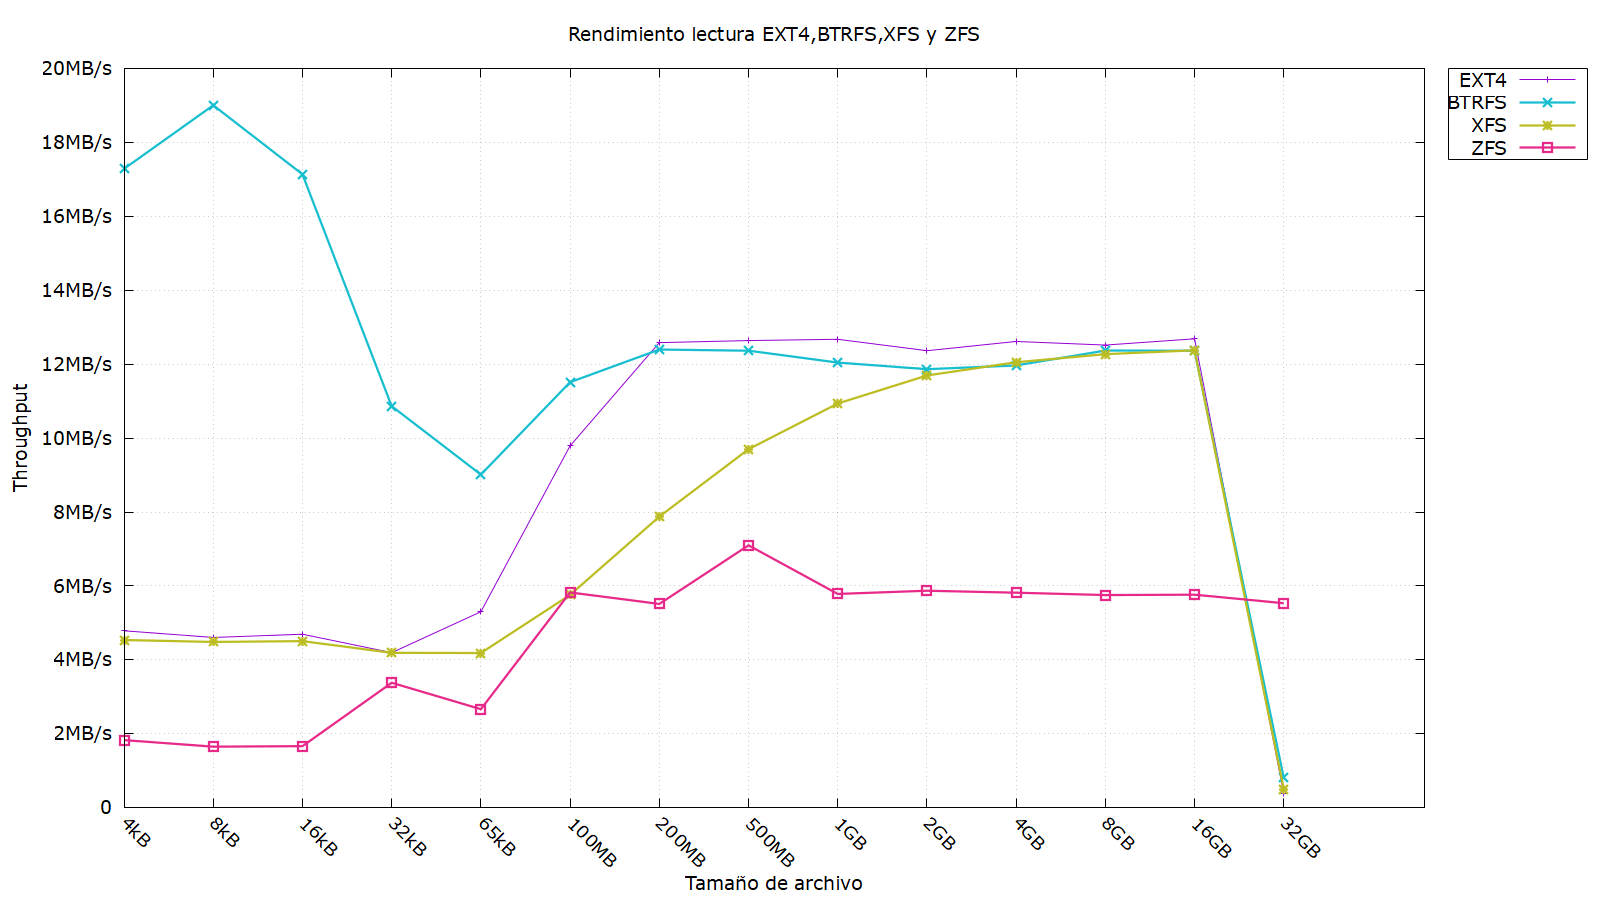
\includegraphics[width=1\linewidth]{results/read_throughput_plot.png}
    \caption{Rendimiento de lectura de ext4, Btrfs, XFS y ZFS en MB/s}
    \label{fig:lectura_throughput}
\end{figure}

Podemos apreciar también cómo, conforme aumenta el tamaño del fichero, aumenta el throughput obtenido, llegando al punto máximo de la controladora. Este punto máximo indica el máximo de bytes por segundo que el disco puede suministrar al sistema operativo en ese momento. Este punto está en torno a los 12 MB/s, y podemos ver cómo ext4 y Btrfs alcanzan este rendimiento al mismo tiempo, alrededor de los 200 MB de tamaño de fichero. XFS, en cambio, obtiene el rendimiento máximo de la controladora en torno a los 8 GB de tamaño de archivo. \\

\begin{table}[h!]
\centering
\caption{Rendimiento de lectura de ext4, Btrfs, XFS y ZFS en MB/s}
\begin{tabular}{|l|c|c|c|c|}
\hline
\textbf{Métrica} & \textbf{ext4} & \textbf{Btrfs} & \textbf{XFS} & \textbf{ZFS} \\ \hline
Mínimo           & 0,38 MB/s     & 0,80 MB/s      & 0,50 MB/s    & 5,53 MB/s \\ \hline
Máximo           & 12,69 MB/s    & 19,01 MB/s     & 12,38 MB/s   & 7,75 MB/s \\ \hline
Promedio         & 8,70 MB/s     & 12,21 MB/s     & 7,50 MB/s    & 4,58 MB/s \\ \hline
Desviación Típica & 4,44 MB/s     & 4,29 MB/s      & 3,95 MB/s    & 1,90 MB/s \\ \hline
\end{tabular}
\label{tab:rendimiento_lectura_sistemas_archivos}
\end{table}

ZFS, por su parte, no llega a alcanzar el rendimiento máximo de la controladora del disco. Esto se debe a la lógica detrás del propio sistema de ficheros, viéndose afectado por las técnicas de integridad como los checksums. Estos no solo se aplican en las operaciones de escritura; de hecho, cuando se solicitan leer datos del disco en el caso de ZFS, antes de devolver los datos a la aplicación, ZFS necesita calcular el checksum que da integridad al bloque, y una vez calculado, necesita ser comparado con el checksum almacenado en sus metadatos. \\

Podríamos pensar que las cachés agilizarían estas lecturas, pero esta aceleración no es tan significativa como en los demás sistemas de ficheros. Incluso en el caso de que los datos solicitados estén en la caché, ZFS aún realiza una verificación del checksum para asegurarse de que los datos en la memoria no estén corruptos. \\

Hemos observado, además, cómo la caché del sistema, que en este caso era de 32 GB, solo llegaba a dedicar 16 GB para el buffer caché y la caché de páginas. Es decir, aun teniendo espacio disponible para almacenar bloques de disco en memoria, el máximo que permitía aumentar esa caché el sistema operativo era de 16 GB. Aunque este parámetro puede ser modificado cambiando configuraciones del kernel, por lo general este tipo de caché se suele limitar a la mitad del tamaño total de memoria RAM del equipo. \\

Podemos apreciar también cómo los tres sistemas de ficheros que llegan al máximo rendimiento de la controladora, ext4, Btrfs y XFS, y que, por tanto, llenan la caché con bloques de disco, sufren una caída de rendimiento en el salto de 16 GB a 32 GB. Esto se debe a la necesidad de traer nuevos bloques de disco a la caché y a su vez desalojar otros por falta de espacio. Además, el hecho de generar un gran número de solicitudes de lectura simultáneas para traer esos bloques faltantes hace que se sature la cola de la controladora de disco, reduciendo el rendimiento significativamente en la marca de 32 GB de tamaño de fichero. \\

Cabría esperar que la caída del rendimiento de ZFS se produjese más adelante, quizá en el salto de 32 GB a 64 GB, pero el análisis de este escenario implica una carga de trabajo que sería más apropiada para una tesis doctoral y de una forma más detallada que el trabajo de fin de grado.

\subsection{Relectura}

En el caso de la relectura, podemos apreciar cómo nuevamente Btrfs se beneficia de un rendimiento que triplica para tamaños de fichero muy pequeños, desde 4 kB hasta 32 kB. Una vez pasado este umbral, el rendimiento se estabiliza y se alcanza el máximo rendimiento de la controladora para este sistema de ficheros.\\

Específicamente, Btrfs alcanza el rendimiento máximo de la controladora con archivos de apenas 32 kB, antes incluso que en la prueba de lectura secuencial, donde se alcanzaba con archivos de 200 MB. Mientras tanto, ext4 y XFS logran este pico con archivos cercanos a los 100 MB, ligeramente antes que en la prueba de lectura secuencial. Este fenómeno se presenta mucho antes en la relectura debido al uso efectivo de las cachés, cuyo impacto es tan significativo que los sistemas ext4, XFS y Btrfs muestran un rendimiento prácticamente idéntico a partir de los 100 MB de tamaño de fichero. El pico de rendimiento de la controladora, que asciende a 12 MB/s, es consistente con los observados en las pruebas de lectura secuencial.\\

Una vez más, se observa que las cachés pierden efectividad cuando el tamaño del archivo supera los 16 GB, resultando en una abrupta caída del rendimiento al escalar hasta los 32 GB. Esto se debe a la necesidad de desalojar páginas de la memoria caché para alojar otras nuevas, produciendo fallos al traer bloques de disco a memoria y penalizando el rendimiento, que disminuye hasta prácticamente 1 MB/s.\\

Al igual que en la prueba de lectura secuencial, ZFS muestra un rendimiento considerablemente menor en comparación con otros sistemas de ficheros debido a su cifrado y sus métodos de respaldo. Sin embargo, destaca por no experimentar una caída pronunciada en el rendimiento al pasar de archivos de 16 GB a 32 GB. Esto se debe a que, al no agotar el tamaño de la caché, aún tiene margen para almacenar en ella bloques de disco. Podemos suponer que este sistema alcanzaría su punto más bajo en saltos superiores a los 32 GB, probablemente en el de 32 GB a 64 GB de tamaño de archivo.\\

\begin{figure}[h!]
    \centering
    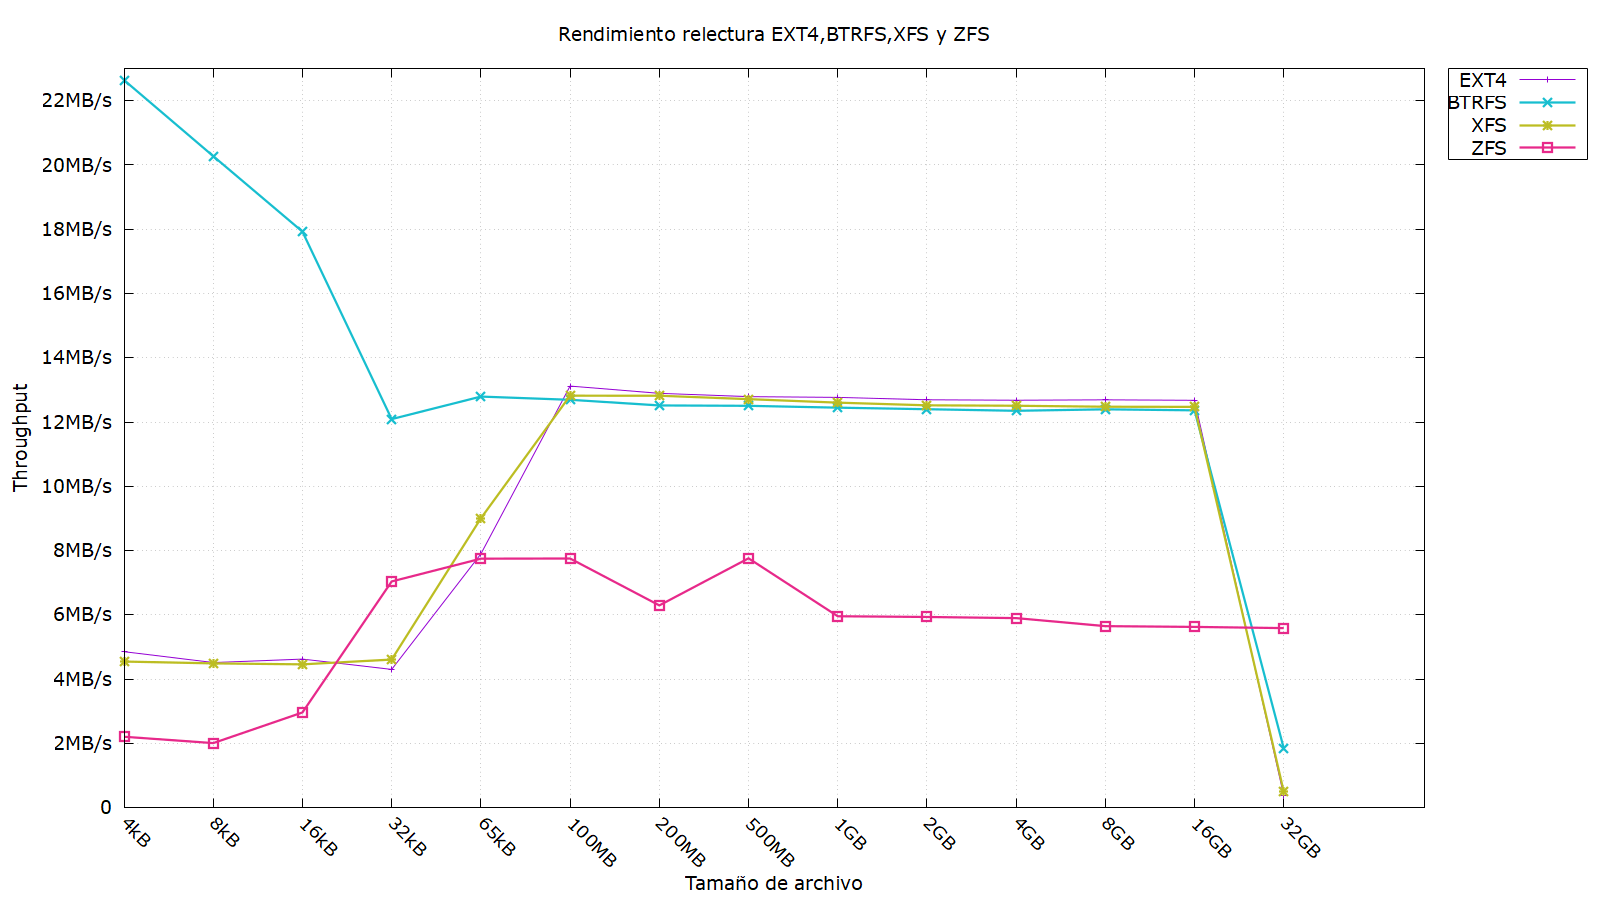
\includegraphics[width=1\linewidth]{results/reread_throughput_plot.png}
    \caption{Rendimiento de relectura de ext4, Btrfs, XFS y ZFS en MB/s}
    \label{fig:relectura_throughput}
\end{figure}

\begin{table}[h!]
\centering
\caption{Rendimiento de relectura de ext4, Btrfs, XFS y ZFS en MB/s}
\begin{tabular}{|l|c|c|c|c|}
\hline
\textbf{Métrica} & \textbf{ext4} & \textbf{Btrfs} & \textbf{XFS} & \textbf{ZFS} \\ \hline
Mínimo           & 0,37 MB/s     & 1,85 MB/s      & 0,50 MB/s    & 5,59 MB/s \\ \hline
Máximo           & 12,69 MB/s    & 22,64 MB/s     & 12,82 MB/s   & 7,75 MB/s \\ \hline
Promedio         & 9,20 MB/s     & 13,37 MB/s     & 9,18 MB/s    & 5,60 MB/s \\ \hline
Desviación Típica & 4,55 MB/s     & 4,77 MB/s      & 4,44 MB/s    & 1,92 MB/s \\ \hline
\end{tabular}
\label{tab:rendimiento_relectura_sistemas_archivos}
\end{table}

\subsection{Lectura estratificada}

Una vez más, debido al tamaño de bloque seleccionado en las pruebas, vemos cómo se repite el caso en el que hasta los 8 kB de tamaño de fichero, el rendimiento de Btrfs va subiendo. Esto, como ya hemos comentado en las gráficas de lecturas previas, se debe a la lectura multisector. \\

En la prueba de lectura estratificada, observamos que el rendimiento máximo del sistema en el caso de Btrfs se alcanza con archivos de aproximadamente 32 kB, beneficiándose nuevamente de la subasignación de bloques. A partir de ese momento, la caché comienza a actuar de forma significativa y provoca una aceleración en cada uno de los sistemas de archivos. \\

Dado que esta prueba lee con un comportamiento escalonado, el rendimiento pico se alcanza antes que en las demás lecturas, fomentando la aceleración del caché debido a un mayor número de aciertos en la memoria. En lugar de leer datos de manera secuencial, el acceso escalonado lee bloques de datos de forma discontinua. Por ejemplo, el programa puede leer un bloque de datos, saltar varios bloques, leer otro bloque, y así sucesivamente. Si el tamaño del bloque es de 4 KB y el stride es de 16 KB, Iozone leerá 4 KB, luego saltará 16 KB, leerá los siguientes 4 KB, y así sucesivamente. \\

De este modo, a partir de los 65 kB, ext4, Btrfs y XFS muestran una estabilización en el pico de rendimiento, limitándose entonces a la máxima capacidad que la controladora puede ofrecer en esos momentos. A diferencia de las pruebas de lectura anteriores, y debido a la naturaleza no secuencial de la prueba, ZFS presenta un descenso en el rendimiento al pasar del tamaño de fichero de 500 MB a 1 GB, y estabilizándose a partir de ese momento. Esto se puede deber a los mecanismos internos de implementación de ZFS, ya que, por lo que intuimos, la compresión y actualización de los metadatos a partir de estos tamaños penaliza gravemente el rendimiento del sistema de ficheros. Es por esto que el rendimiento a partir de 1 GB de tamaño de archivo se estabiliza. \\

\begin{figure}[h!]
    \centering
    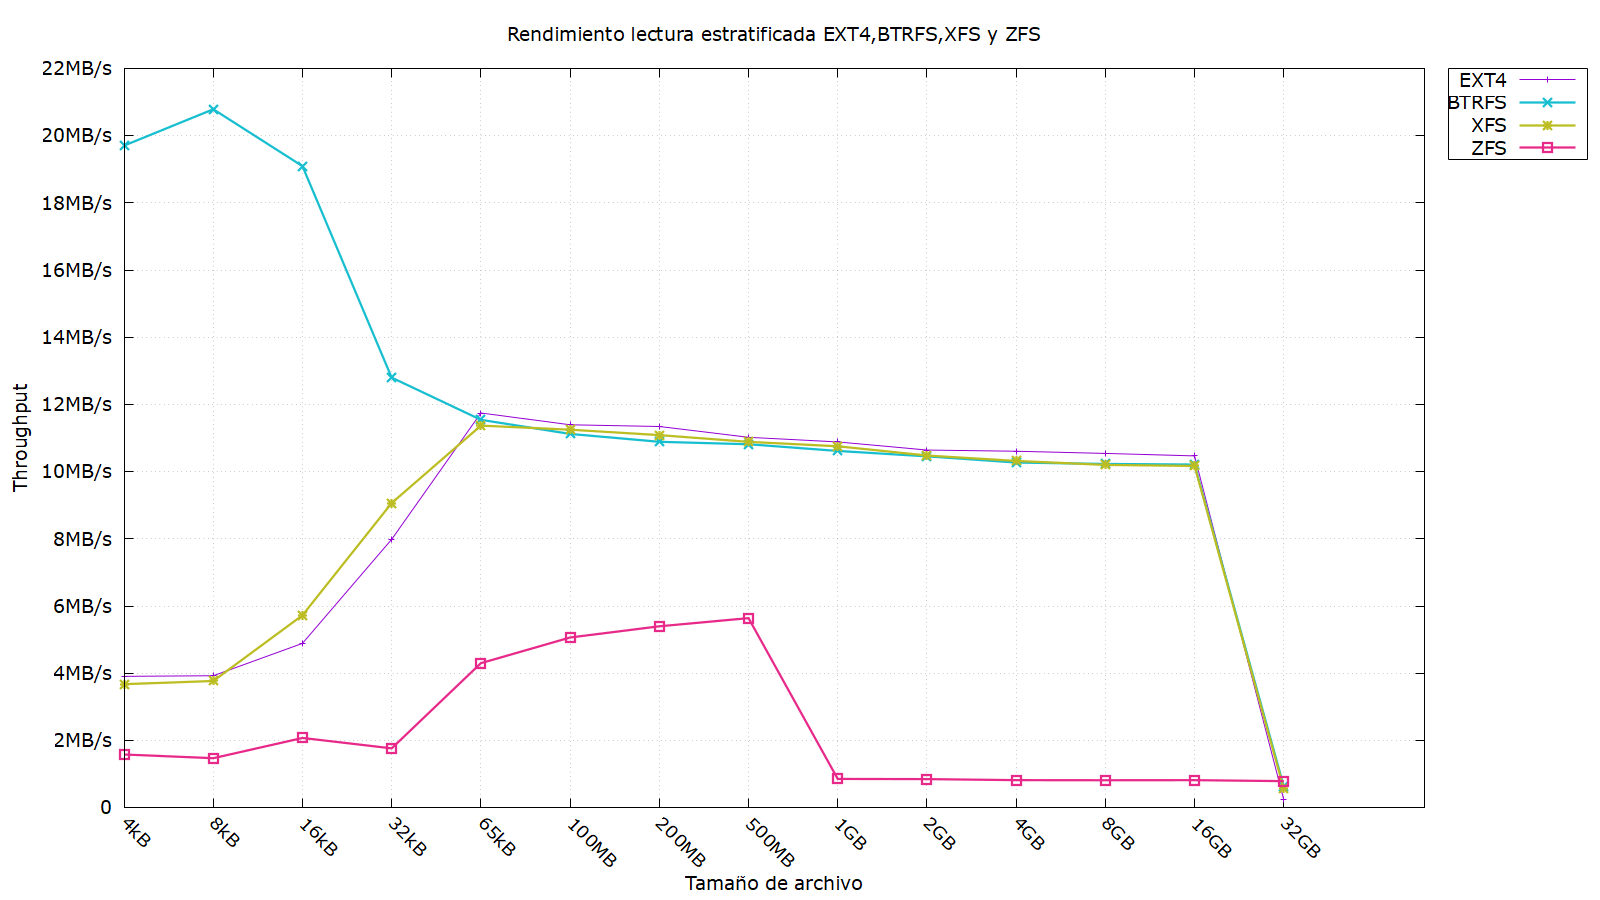
\includegraphics[width=1\linewidth]{results/strided_read_throughput_plot.png}
    \caption{Rendimiento de lectura estratificada de ext4, Btrfs, XFS y ZFS en MB/s}
    \label{fig:lectura_estratificada_throughput}
\end{figure}

\begin{table}[h!]
\centering
\caption{Rendimiento de lectura estratificada de ext4, Btrfs, XFS y ZFS en MB/s}
\begin{tabular}{|l|c|c|c|c|}
\hline
\textbf{Métrica} & \textbf{ext4} & \textbf{Btrfs} & \textbf{XFS} & \textbf{ZFS} \\ \hline
Mínimo           & 0,24 MB/s     & 0,63 MB/s      & 0,56 MB/s    & 0,79 MB/s \\ \hline
Máximo           & 11,75 MB/s    & 20,79 MB/s     & 11,37 MB/s   & 5,65 MB/s \\ \hline
Promedio         & 8,54 MB/s     & 12,08 MB/s     & 8,52 MB/s    & 2,30 MB/s \\ \hline
Desviación Típica & 3,72 MB/s     & 5,07 MB/s      & 3,54 MB/s    & 1,90 MB/s \\ \hline
\end{tabular}
\label{tab:rendimiento_lectura_estratificada_sistemas_archivos}
\end{table}

\subsection{Lectura aleatoria}

Al igual que en las demás pruebas, Btrfs destaca en tamaños de fichero muy pequeños, alcanzando el rendimiento pico de la controladora en torno a los 65 kB. Como en otras pruebas de lectura, la subasignación de bloques de Btrfs juega un papel crucial al mejorar el rendimiento con archivos de tamaño muy pequeño.

Podemos comprobar también cómo, para los sistemas de ficheros ext4 y XFS, el rendimiento máximo de la controladora se alcanza con archivos de 65 kB. Sin embargo, debido a la aleatoriedad de esta prueba específica, observamos que el rendimiento disminuye gradualmente en lugar de estabilizarse. Esto ocurre porque los datos solicitados eventualmente dejan de estar disponibles en la caché y necesitan ser traídos a la memoria, lo que ralentiza el proceso y resulta en una pérdida de la aceleración que la caché proporciona. \\

Al igual que en las pruebas de lectura anteriores, notamos una caída significativa en el rendimiento al pasar de 16 GB a 32 GB de datos. Es especialmente interesante observar cómo ZFS muestra una disminución drástica en el rendimiento a partir de archivos de 1 GB, resaltando nuevamente la penalización que sufre debido al algoritmo de integridad que presenta. \\

Una vez más, ext4, Btrfs y XFS presentan una caída drástica de rendimiento al pasar de 16 GB a 32 GB. Esto se debe a que la caché está llena y las solicitudes al disco se vuelven inmanejables, resultando en un rendimiento de aproximadamente 1 MB/s.

\begin{figure}[h!]
    \centering
    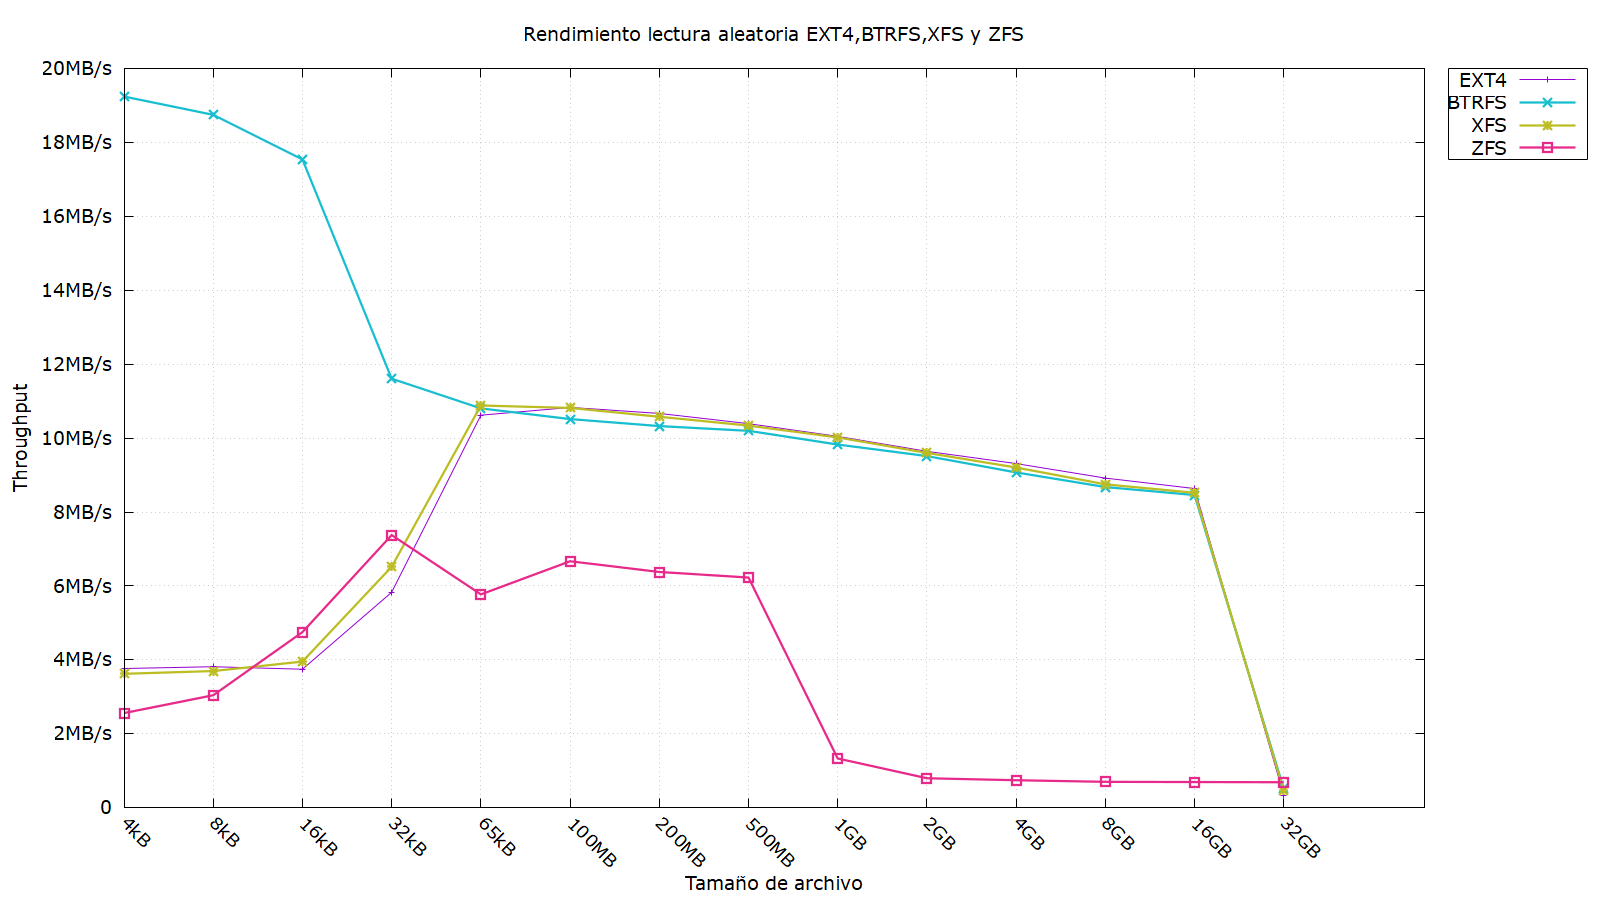
\includegraphics[width=1\linewidth]{results/random_read_throughput_plot.png}
    \caption{Rendimiento de lectura aleatoria de ext4, Btrfs, XFS y ZFS en MB/s}
    \label{fig:lectura_aleatoria_throughput}
\end{figure}

\begin{table}[h!]
\centering
\caption{Rendimiento de lectura aleatoria de ext4, Btrfs, XFS y ZFS en MB/s}
\begin{tabular}{|l|c|c|c|c|}
\hline
\textbf{Métrica} & \textbf{ext4} & \textbf{Btrfs} & \textbf{XFS} & \textbf{ZFS} \\ \hline
Mínimo           & 0,34 MB/s     & 0,51 MB/s      & 0,46 MB/s    & 0,69 MB/s \\ \hline
Máximo           & 10,82 MB/s    & 19,24 MB/s     & 10,88 MB/s   & 7,38 MB/s \\ \hline
Promedio         & 7,61 MB/s     & 11,07 MB/s     & 7,64 MB/s    & 3,41 MB/s \\ \hline
Desviación Típica & 3,42 MB/s     & 4,82 MB/s      & 3,38 MB/s    & 2,66 MB/s \\ \hline
\end{tabular}
\label{tab:rendimiento_lectura_aleatoria_sistemas_archivos}
\end{table}

\newpage

\section{Pruebas de escritura}
\subsection{Escritura}

Una vez más, Btrfs destaca incrementando su rendimiento hasta el tamaño de bloque de 8 kB, debido principalmente a la escritura multisector, que permite enviar las escrituras que son más pequeñas que el tamaño de bloque, en este caso 8 kB, en una sola operación, mejorando significativamente el rendimiento.\\

Además, Btrfs sobresale en los tamaños de fichero pequeños gracias a la implementación de técnicas como la escritura retrasada (delayed write), la compartición de bloques y la escritura coalescente, previamente referenciadas en las características de Btrfs, que optimizan el rendimiento de las escrituras.\\

Ambas técnicas, escritura retrasada y coalescente, son implementadas por Btrfs y explican el rendimiento sobresaliente que obtiene para las escrituras de archivos pequeños. La escritura retrasada permite acumular datos en la caché, y durante ese tiempo, la escritura coalescente puede agrupar estas operaciones en bloques más grandes antes de escribirlos en el disco, maximizando así la eficiencia y el rendimiento.\\

La compartición de bloques en Btrfs también contribuye significativamente a la optimización de las escrituras. Esta técnica permite un uso más eficiente del espacio en disco y reduce la cantidad de escrituras necesarias.\\

Btrfs también se beneficia en la escritura gracias a su estructura interna basada en árboles B+. Las escrituras en una estructura arborescente son mucho más eficientes que las que deben modificar bitmaps, como es el caso de ext4, XFS y ZFS.\\

Podemos observar cómo tanto ext4, Btrfs y XFS presentan caídas pronunciadas en su rendimiento después de alcanzar su pico. Estas caídas se deben principalmente a que la memoria caché se agota, obligando a enviar las peticiones a la cola de disco, lo que causa saturación y un rendimiento reducido.\\

Es notable que ZFS, al igual que en las pruebas anteriores, no alcanza su rendimiento máximo, sino que se mantiene estable a partir de los 200 MB de tamaño de fichero. También es destacable que su rendimiento no decae en los tamaños de fichero más grandes, a diferencia de ext4, Btrfs y XFS. Esto se debe a que ZFS gestiona la caché de manera más eficiente, asegurando la integridad de las operaciones de lectura.\\

Btrfs presenta una caída menos acentuada en comparación con ext4 y XFS, lo cual se atribuye a la mencionada escritura multisector, que agrupa las escrituras y evita que la cola de disco se sature a niveles críticos. \\

\begin{figure}[h!]
    \centering
    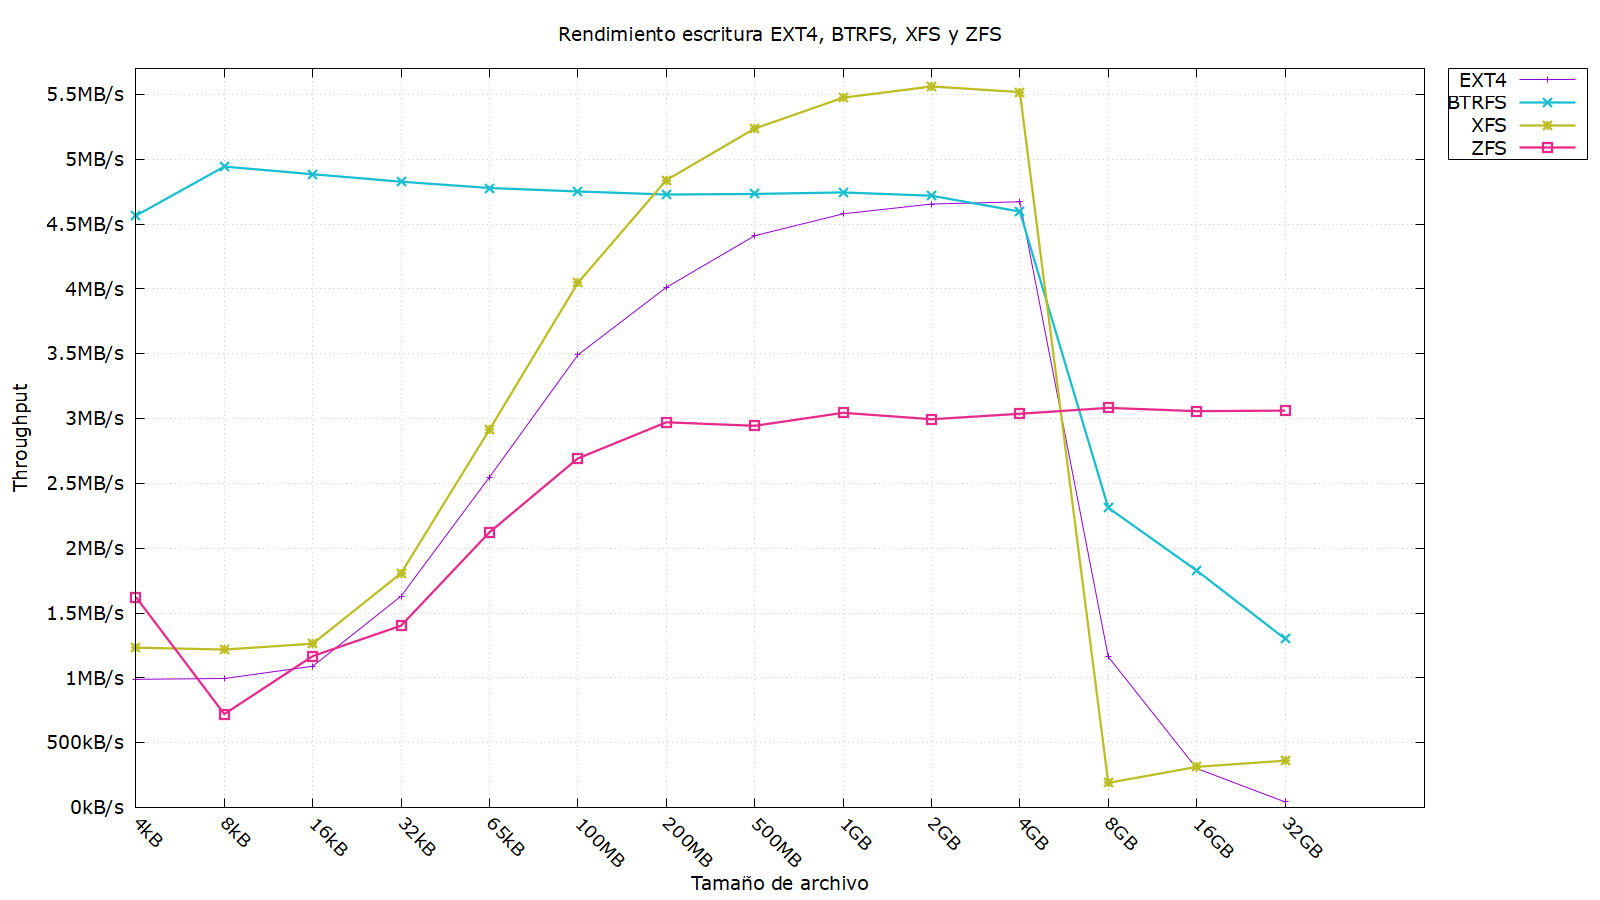
\includegraphics[width=1\linewidth]{results/write_throughput_plot.png}
    \caption{Rendimiento de escritura de ext4, Btrfs, XFS y ZFS en MB/s}
    \label{fig:escritura_throughput}
\end{figure}

\begin{table}[h!]
    \centering
    \caption{Rendimiento de escritura de ext4, Btrfs, XFS y ZFS en MB/s}
    \begin{tabular}{|l|c|c|c|c|}
        \hline
        \textbf{Métrica}  & \textbf{ext4} & \textbf{Btrfs} & \textbf{XFS}  & \textbf{ZFS}  \\ \hline
        Mínimo            & 0,99 MB/s   & 4,57 MB/s   & 1,23 MB/s   & 1,62 MB/s  \\ \hline
        Máximo            & 4,67 MB/s & 4,94 MB/s  & 5,47 MB/s & 3,04 MB/s \\ \hline
        Promedio          & 2,90 MB/s & 4,03 MB/s  & 2,79 MB/s & 2,38 MB/s  \\ \hline
        Desviación Típica & 1,69 MB/s  & 1,31 MB/s   & 2,21 MB/s  & 0,83 MB/s  \\ \hline
    \end{tabular}
    \label{tab:rendimiento_escritura_sistemas_archivos}
\end{table}

En comparación, XFS muestra el mejor rendimiento en las escrituras de archivos grandes, debido principalmente a los grupos de asignación. Los grupos de asignación en XFS permiten que el sistema de archivos gestione sus inodos y espacio libre de forma independiente por cada grupo, posibilitando que múltiples hilos realicen operaciones de escritura simultáneamente sin interferencia, lo que es ideal para aplicaciones que manejan grandes volúmenes de datos.

\subsection{Reescritura}

En el caso de la reescritura, el rendimiento observado supera en todos los casos al de la escritura secuencial, gracias a varios factores clave en la gestión de datos. Primero, no es necesario recrear la tabla de asignación de bloques porque esta ya existe y se mantiene intacta, lo que elimina una operación significativa que consume tiempo. \\

El segundo elemento crucial es la escritura diferida. Normalmente, el intervalo para desencadenar estas escrituras consolidadas es de aproximadamente 30 segundos, aunque puede variar según la configuración del sistema y las circunstancias operativas. Durante operaciones de reescritura, este contador puede retrasarse aún más, reiniciándose si el bloque que se va a escribir aún está en memoria. Esto permite que las operaciones de escritura se agrupen, reduciendo la carga inmediata sobre el disco. \\

Podemos apreciar además que, en el caso de ext4, Btrfs y XFS, es notorio el uso de la escritura diferida. Es importante destacar cómo en este caso, la memoria que el sistema es capaz de dedicar al caché es el limitante, pues como podemos comprobar, una vez el caché está lleno, en el salto de 16GB a 32GB de tamaño de archivo, las escrituras son encoladas al disco, lo que reduce el rendimiento a prácticamente 1MB/s. \\

ZFS, en cambio, presenta un rendimiento estable casi durante toda la prueba, destacándose por no caer en el salto de los 16GB a 32GB de tamaño de fichero. Esto se debe a que la memoria caché realmente no está llena, ya que los algoritmos de compresión e integridad del propio sistema de archivos hacen que las escrituras se envíen a disco y se desalojen páginas del caché. Podríamos decir que, en el caso de este sistema de archivos, los recursos están compartidos de forma equitativa, pues no solo depende de la capacidad del disco para servir a la memoria de bloques, sino que la penalización de la compresión también involucra a la CPU y otros recursos del sistema.

\begin{figure}[h!]
    \centering
    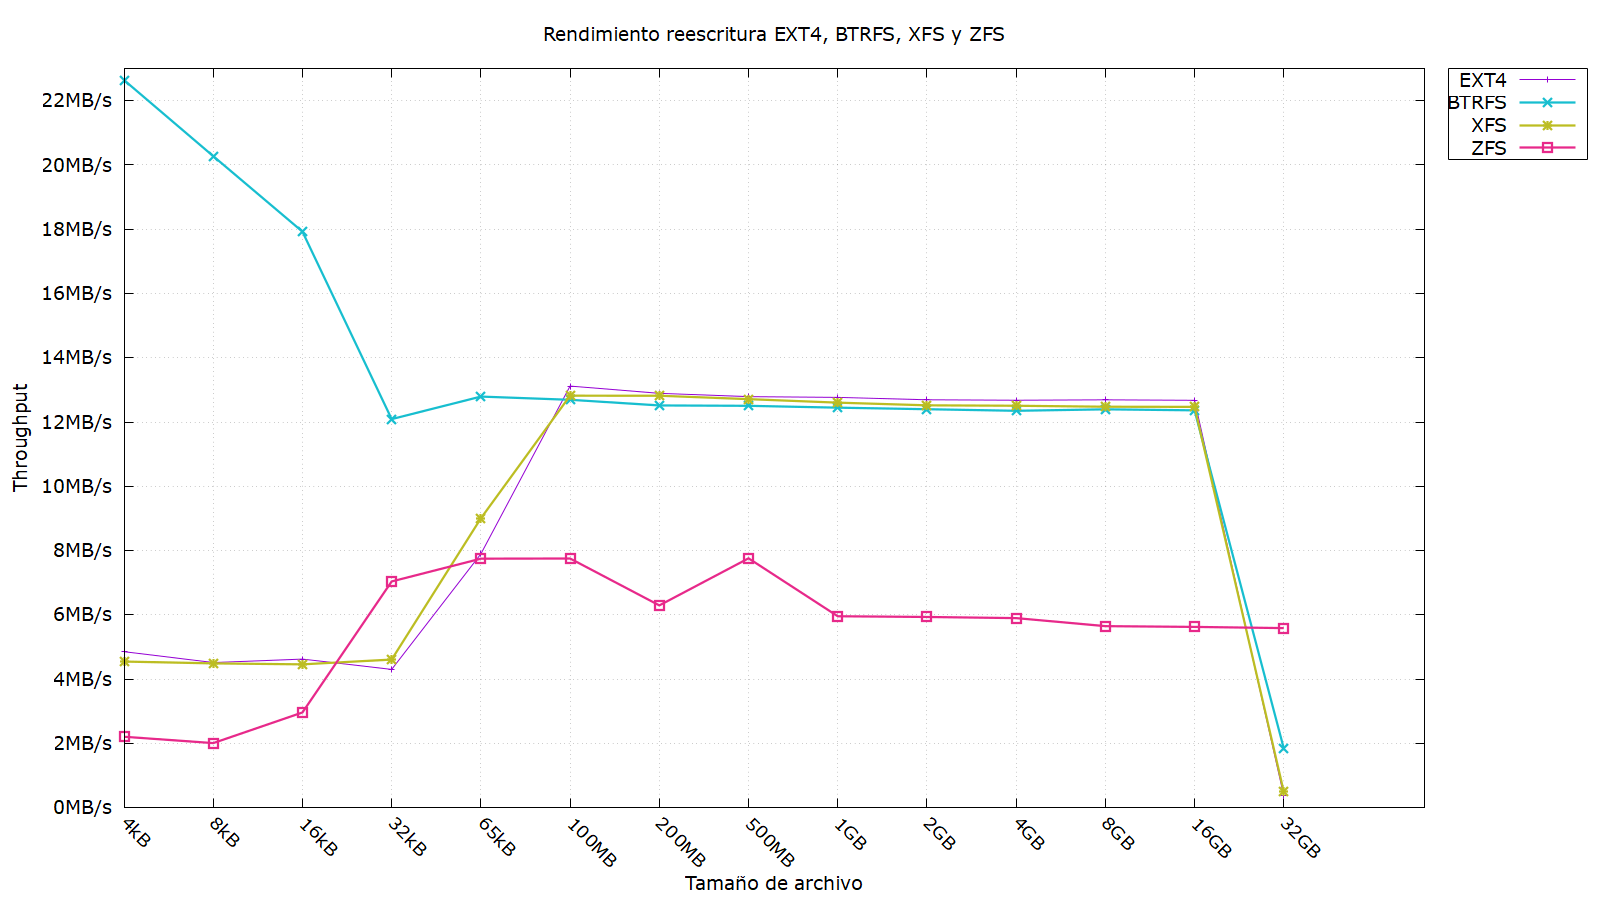
\includegraphics[width=1\linewidth]{results/rewrite_throughput_plot.png}
    \caption{Rendimiento de reescritura de ext4, Btrfs, XFS y ZFS en MB/s}
    \label{fig:reescritura_throughput}
\end{figure}

\begin{table}[h!]
    \centering
    \caption{Rendimiento de reescritura de ext4, Btrfs, XFS y ZFS en MB/s}
    \begin{tabular}{|l|c|c|c|c|}
    \hline
    \textbf{Métrica} & \textbf{ext4} & \textbf{Btrfs} & \textbf{XFS} & \textbf{ZFS} \\ \hline
    Mínimo           & 0,37 MB/s     & 1,85 MB/s      & 0,50 MB/s    & 2,01 MB/s \\ \hline
    Máximo           & 13,12 MB/s    & 22,64 MB/s     & 12,82 MB/s   & 7,76 MB/s \\ \hline
    Promedio         & 9,20 MB/s     & 13,37 MB/s     & 9,18 MB/s    & 5,60 MB/s \\ \hline
    Desviación Típica & 4,55 MB/s    & 4,77 MB/s      & 4,44 MB/s    & 1,92 MB/s \\ \hline
    \end{tabular}
    \label{tab:rendimiento_reescritura_sistemas_archivos}
\end{table}

\subsection{Escritura aleatoria}

Al igual que en las demás escrituras, Btrfs presenta un rendimiento sobresaliente en comparación con otros sistemas de archivos. Esto se debe, como mencionamos previamente, a sus técnicas de escritura diferida, compartición de bloques y escritura coalescente. \\

Podemos observar que, prácticamente desde el comienzo, Btrfs alcanza su rendimiento máximo y, a partir de ahí, su rendimiento disminuye. Esta disminución también afecta a los demás sistemas de archivos y se debe a la propia aleatoriedad intrínseca de la prueba. En otras palabras, perdemos gran parte de la aceleración generada por la caché debido a los numerosos fallos en memoria. Además, esto provoca que la escritura diferida no se vea reseteada y envíe las escrituras al disco de manera anticipada, produciendo un descenso mucho más rápido que en las pruebas anteriores, aproximadamente a partir de los 65 kB. \\

Podemos comprobar también cómo tanto ext4, Btrfs y XFS presentan un rendimiento prácticamente idéntico a partir de los 65 kB, incluso destacando XFS por aproximadamente 0,5 MB en los mejores casos. ZFS, en cambio, sigue la línea de las pruebas anteriores, pero presenta un rendimiento bastante mejor en archivos pequeños, específicamente para 16 kB. \\

\begin{figure}[h!]
    \centering
    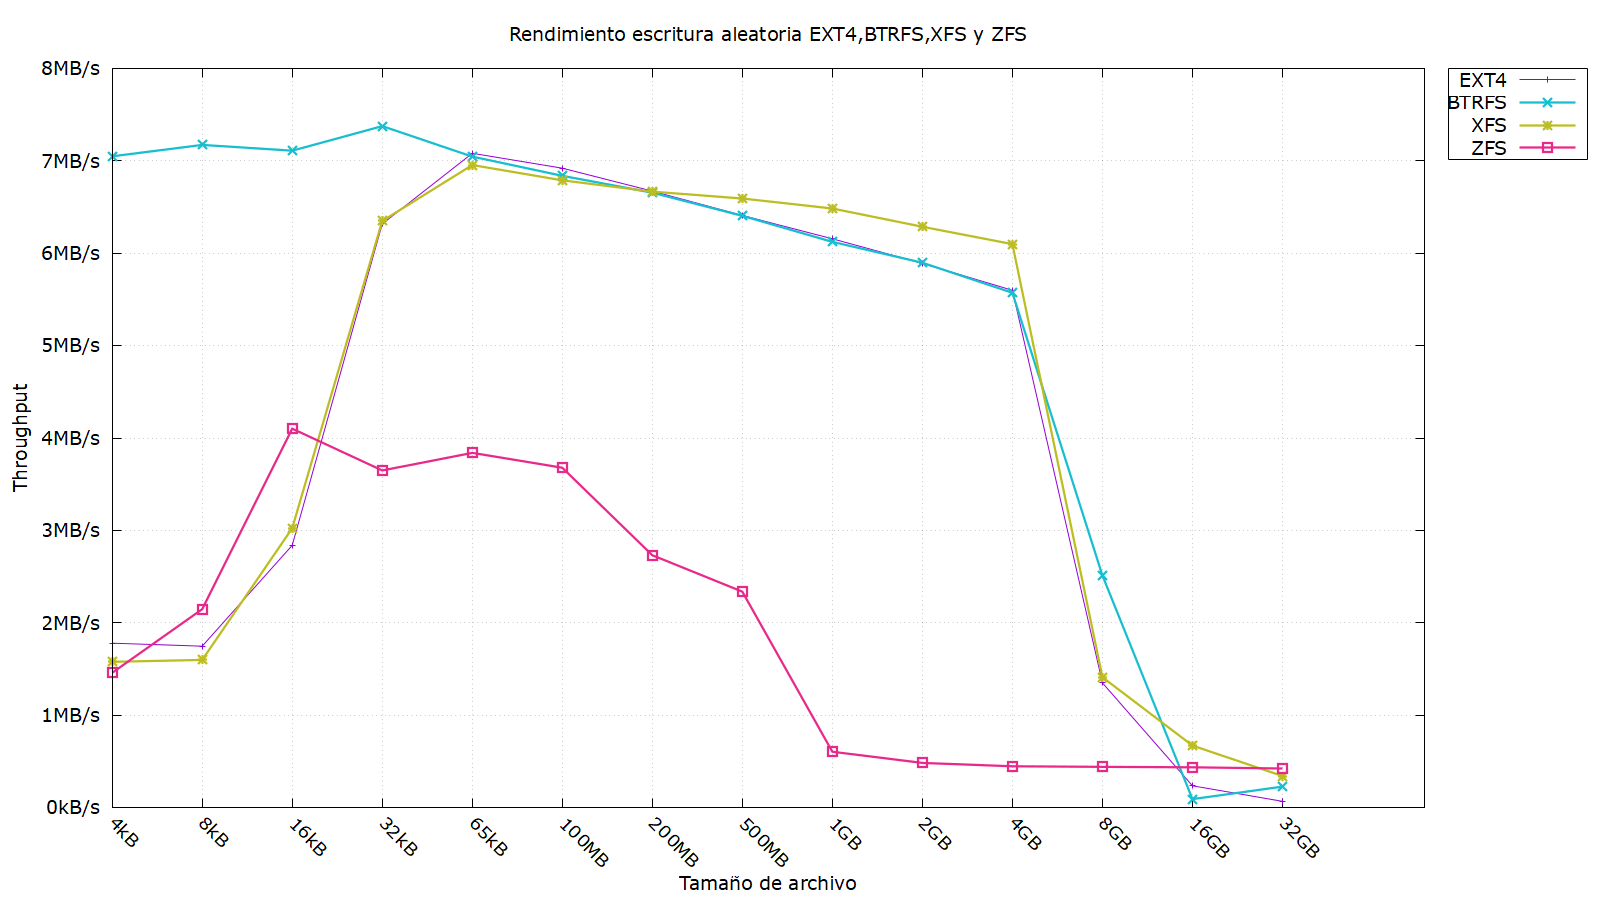
\includegraphics[width=1\linewidth]{results/random_write_throughput_plot.png}
    \caption{Rendimiento de escritura aleatoria de ext4, Btrfs, XFS y ZFS en MB/s}
    \label{fig:escritura_aleatoria_throughput}
\end{figure}

\begin{table}[h!]
\centering
\caption{Rendimiento de escritura aleatoria de ext4, Btrfs, XFS y ZFS en MB/s}
\begin{tabular}{|l|c|c|c|c|}
\hline
\textbf{Métrica} & \textbf{ext4} & \textbf{Btrfs} & \textbf{XFS} & \textbf{ZFS} \\ \hline
Mínimo           & 0,07 MB/s     & 0,09 MB/s      & 0,34 MB/s    & 0,42 MB/s \\ \hline
Máximo           & 7,08 MB/s     & 7,37 MB/s      & 6,96 MB/s    & 4,10 MB/s \\ \hline
Promedio         & 4,22 MB/s     & 5,43 MB/s      & 4,35 MB/s    & 1,91 MB/s \\ \hline
Desviación Típica & 2,70 MB/s     & 2,54 MB/s      & 2,69 MB/s    & 1,47 MB/s \\ \hline
\end{tabular}
\label{tab:rendimiento_escritura_aleatoria_sistemas_archivos}
\end{table}

Encontramos también un descenso abrupto en el rendimiento de Btrfs en la escritura aleatoria, especialmente en archivos pequeños. En este caso, podemos apreciar cómo el rendimiento de ext4, Btrfs y XFS se ve muy afectado por la aleatoriedad de la prueba, produciendo un descenso paulatino conforme el test avanza. Este descenso se debe a la pérdida de gran parte de la aceleración obtenida de la escritura diferida, ya que en este caso la caché se ve obligada a enviar las solicitudes de escritura al disco sin poder agrupar las escrituras coalescentes.







% Chapter 6: Results conclusions
\chapter{Conclusiones de los Resultados}

Este capítulo presenta las conclusiones derivadas de las pruebas de rendimiento de los sistemas de archivos Btrfs, Ext4, XFS y ZFS, evaluando sus capacidades y limitaciones bajo diferentes condiciones de uso. A continuación, se destacan los hallazgos principales y se justifican los resultados obtenidos.

\section{Rendimiento en Lectura}

En las pruebas de lectura, \textbf{Btrfs mostró un rendimiento superior en la lectura de archivos pequeños}, alcanzando un promedio de 12.21 MB/s, lo que representa un 40\% más que Ext4 y un 63\% más que XFS. ZFS, aunque se beneficia de sus características de integridad y cifrado, tuvo un rendimiento promedio significativamente menor (4.58 MB/s), penalizado por sus algoritmos de cifrado e integridad.

\begin{table}[h!]
\centering
\caption{Comparación de rendimiento en lectura}
\begin{tabular}{|l|c|c|c|c|}
\hline
\textbf{Métrica} & \textbf{EXT4} & \textbf{Btrfs} & \textbf{XFS} & \textbf{ZFS} \\ \hline
Promedio (MB/s)   & 8.70          & \textbf{12.21} & 7.50         & 4.58         \\ \hline
Mejora vs EXT4    & -             & \textbf{40\%}  & -14\%        & -47\%        \\ \hline
Mejora vs Btrfs   & -29\%         & -              & -39\%        & -62\%        \\ \hline
Mejora vs XFS     & 16\%          & \textbf{63\%}  & -            & -39\%        \\ \hline
Mejora vs ZFS     & 90\%          & \textbf{167\%} & 64\%         & -            \\ \hline
\end{tabular}
\end{table}

\section{Rendimiento en Relectura}

En las pruebas de relectura, \textbf{Btrfs nuevamente destacó}, alcanzando un promedio de rendimiento de 13.37 MB/s, superando en un 45\% a Ext4 y en un 46\% a XFS. La eficiencia de la subasignación de bloques y la gestión de caché contribuyeron a estos resultados. ZFS, aunque mejoró respecto a la lectura (5.60 MB/s), continuó mostrando un rendimiento inferior debido a sus métodos de respaldo y cifrado.

\begin{table}[h!]
\centering
\caption{Comparación de rendimiento en relectura}
\begin{tabular}{|l|c|c|c|c|}
\hline
\textbf{Métrica} & \textbf{EXT4} & \textbf{Btrfs} & \textbf{XFS} & \textbf{ZFS} \\ \hline
Promedio (MB/s)   & 9.20          & \textbf{13.37} & 9.18         & 5.60         \\ \hline
Mejora vs EXT4    & -             & \textbf{45\%}  & 0\%          & -39\%        \\ \hline
Mejora vs Btrfs   & -31\%         & -              & -31\%        & -58\%        \\ \hline
Mejora vs XFS     & 0\%           & \textbf{46\%}  & -            & -39\%        \\ \hline
Mejora vs ZFS     & 64\%          & \textbf{139\%} & 64\%         & -            \\ \hline
\end{tabular}
\end{table}

\section{Rendimiento en Lectura Estratificada}

\textbf{Btrfs se destacó nuevamente en las pruebas de lectura estratificada}, alcanzando un promedio de rendimiento de 12.08 MB/s, superando en un 41\% a Ext4 y en un 42\% a XFS. La eficiencia de la subasignación de bloques y la gestión de caché contribuyeron a estos resultados. ZFS, aunque mejoró respecto a la lectura (2.30 MB/s), continuó mostrando un rendimiento inferior debido a sus métodos de respaldo y cifrado.

\begin{table}[h!]
\centering
\caption{Comparación de rendimiento en lectura estratificada}
\begin{tabular}{|l|c|c|c|c|}
\hline
\textbf{Métrica} & \textbf{EXT4} & \textbf{Btrfs} & \textbf{XFS} & \textbf{ZFS} \\ \hline
Promedio (MB/s)   & 8.54          & \textbf{12.08} & 8.52         & 2.30         \\ \hline
Mejora vs EXT4    & -             & \textbf{41\%}  & 0\%          & -73\%        \\ \hline
Mejora vs Btrfs   & -29\%         & -              & -29\%        & -81\%        \\ \hline
Mejora vs XFS     & 0\%           & \textbf{42\%}  & -            & -73\%        \\ \hline
Mejora vs ZFS     & 271\%         & \textbf{425\%} & 270\%        & -            \\ \hline
\end{tabular}
\end{table}

\section{Rendimiento en Lectura Aleatoria}

En las pruebas de lectura aleatoria, \textbf{Btrfs nuevamente destacó}, alcanzando su rendimiento máximo con archivos de 32 kB, significativamente antes que en la prueba de lectura secuencial. El promedio de rendimiento de Btrfs fue de 11.07 MB/s, superando en un 45\% a Ext4 y en un 45\% a XFS. La eficiencia de la subasignación de bloques y la gestión de caché contribuyeron a estos resultados. ZFS, aunque mejoró respecto a la lectura secuencial (3.41 MB/s), continuó mostrando un rendimiento inferior debido a sus métodos de respaldo y cifrado.

\begin{table}[h!]
\centering
\caption{Comparación de rendimiento en lectura aleatoria}
\begin{tabular}{|l|c|c|c|c|}
\hline
\textbf{Métrica} & \textbf{EXT4} & \textbf{Btrfs} & \textbf{XFS} & \textbf{ZFS} \\ \hline
Promedio (MB/s)   & 7.61          & \textbf{11.07} & 7.64         & 3.41         \\ \hline
Mejora vs EXT4    & -             & \textbf{45\%}  & 0\%          & -55\%        \\ \hline
Mejora vs Btrfs   & -31\%         & -              & -31\%        & -69\%        \\ \hline
Mejora vs XFS     & 0\%           & \textbf{45\%}  & -            & -55\%        \\ \hline
Mejora vs ZFS     & 123\%         & \textbf{225\%} & 124\%        & -            \\ \hline
\end{tabular}
\end{table}

\section{Rendimiento en Escritura}

Para las operaciones de escritura, \textbf{Btrfs sobresalió en archivos pequeños}, con un promedio de 4.12 MB/s, superando a Ext4 en un 67\% y a XFS en un 44\%. Esto se debe a su escritura diferida y la compartición de bloques, técnicas que permiten agrupar múltiples operaciones de escritura y optimizar el uso del espacio en disco. XFS mostró el mejor rendimiento en escrituras de archivos grandes debido a sus grupos de asignación, con un rendimiento máximo de 5.56 MB/s.

\begin{table}[h!]
\centering
\caption{Comparación de rendimiento en escritura}
\begin{tabular}{|l|c|c|c|c|}
\hline
\textbf{Métrica} & \textbf{EXT4} & \textbf{Btrfs} & \textbf{XFS} & \textbf{ZFS} \\ \hline
Promedio (MB/s)   & 2.90         & \textbf{4.03}  & 2.79         & 2.38         \\ \hline
Mejora vs EXT4    & -            & \textbf{39.19\%} & -3.52\%    & -17.71\%     \\ \hline
Mejora vs Btrfs   & -28.14\%     & -               & -30.68\%    & -40.87\%     \\ \hline
Mejora vs XFS     & 3.64\%       & \textbf{44.23\%} & -          & -14.69\%     \\ \hline
Mejora vs ZFS     & 21.48\%      & \textbf{68.99\%} & 17.20\%    & -            \\ \hline
\end{tabular}
\end{table}

\section{Rendimiento en Reescritura}

La reescritura mostró un rendimiento superior en todos los sistemas de archivos debido a la eliminación de la necesidad de recrear la tabla de asignación de bloques y la escritura diferida. \textbf{Btrfs lideró nuevamente} con un promedio de 13.37 MB/s, superando a Ext4 en un 45\% y a XFS en un 46\%. ZFS, aunque mejoró, siguió mostrando el rendimiento más bajo (5.60 MB/s).

\begin{table}[h!]
\centering
\caption{Comparación de rendimiento en reescritura}
\begin{tabular}{|l|c|c|c|c|}
\hline
\textbf{Métrica} & \textbf{EXT4} & \textbf{Btrfs} & \textbf{XFS} & \textbf{ZFS} \\ \hline
Promedio (MB/s)   & 9.20          & \textbf{13.37} & 9.18         & 5.60         \\ \hline
Mejora vs EXT4    & -             & \textbf{45\%}  & 0\%          & -39\%        \\ \hline
Mejora vs Btrfs   & -31\%         & -              & -31\%        & -58\%        \\ \hline
Mejora vs XFS     & 0\%           & \textbf{46\%}  & -            & -39\%        \\ \hline
Mejora vs ZFS     & 64\%          & \textbf{139\%} & 64\%         & -            \\ \hline
\end{tabular}
\end{table}

\section{Rendimiento en Escritura Aleatoria}

La escritura aleatoria mostró variaciones significativas en el rendimiento entre los diferentes sistemas de archivos. \textbf{Btrfs lideró nuevamente} con un promedio de 5.43 MB/s, superando a Ext4 en un 29\% y a XFS en un 25\%. ZFS, aunque mejoró, siguió mostrando el rendimiento más bajo (1.91 MB/s).

\begin{table}[h!]
\centering
\caption{Comparación de rendimiento en escritura aleatoria}
\begin{tabular}{|l|c|c|c|c|}
\hline
\textbf{Métrica} & \textbf{EXT4} & \textbf{Btrfs} & \textbf{XFS} & \textbf{ZFS} \\ \hline
Promedio (MB/s)   & 4.22          & \textbf{5.43}  & 4.35         & 1.91         \\ \hline
Mejora vs EXT4    & -             & \textbf{29\%}  & 3\%          & -55\%        \\ \hline
Mejora vs Btrfs   & -22\%         & -              & -20\%        & -65\%        \\ \hline
Mejora vs XFS     & -3\%          & \textbf{25\%}  & -            & -56\%        \\ \hline
Mejora vs ZFS     & 121\%         & \textbf{184\%} & 127\%        & -            \\ \hline
\end{tabular}
\end{table}



% Chapter 7: Conclusions and recommendations
\chapter{Conclusiones y Recomendaciones}

En resumen, \textbf{Btrfs demostró ser el sistema de archivos más eficiente en la gestión de archivos pequeños y en operaciones de relectura y reescritura}, gracias a su técnica de subasignación de bloques y escritura diferida. \textbf{XFS destacó en la gestión de archivos grandes} debido a sus grupos de asignación. \textbf{Ext4 mostró un rendimiento consistente pero inferior a Btrfs y XFS} en la mayoría de las pruebas. \textbf{ZFS, aunque penalizado por sus algoritmos de cifrado e integridad, ofreció una estabilidad notable en su rendimiento}, particularmente en operaciones de relectura.

Estos resultados sugieren que la elección del sistema de archivos debe basarse en las necesidades específicas de uso, considerando el tamaño de los archivos y las operaciones predominantes (lectura, escritura, aleatoria, secuencial) para optimizar el rendimiento del sistema. La implementación de técnicas avanzadas de gestión de caché y optimización de acceso es crucial para maximizar la eficiencia y rendimiento de los sistemas de archivos.

\section{Recomendaciones de Uso Según el Sistema de Archivos}

A continuación, se presentan recomendaciones específicas basadas en los resultados de rendimiento para cada sistema de archivos evaluado:

\subsection{Btrfs}

Para aplicaciones que requieren un manejo eficiente de archivos pequeños y numerosas operaciones de lectura y relectura, \textbf{Btrfs es la opción más adecuada}. Ejemplos de estos casos de uso incluyen:

\begin{itemize}
    \item \textbf{Bases de Datos}: Btrfs es ideal para bases de datos donde las lecturas aleatorias de archivos pequeños son comunes. Su capacidad para manejar eficientemente la fragmentación y su alta velocidad en operaciones de relectura mejoran significativamente el rendimiento.
    \item \textbf{Repositorios de Código Fuente}: En entornos de desarrollo, donde se realizan múltiples operaciones de lectura y escritura de archivos pequeños, Btrfs ofrece ventajas considerables debido a su técnica de subasignación de bloques.
\end{itemize}

\subsection{XFS}

\textbf{XFS se destaca en la gestión de archivos grandes y operaciones de escritura intensiva}. Es especialmente adecuado para:

\begin{itemize}
    \item \textbf{Repositorios de Máquinas Virtuales}: Para entornos de virtualización donde se almacenan imágenes de máquinas virtuales grandes, XFS proporciona un rendimiento superior en escrituras secuenciales y aleatorias de archivos grandes.
    \item \textbf{Sistemas de Almacenamiento de Video}: En aplicaciones que involucran el almacenamiento y procesamiento de grandes archivos de video, XFS es beneficioso debido a su manejo eficiente de grandes volúmenes de datos.
\end{itemize}

\subsection{Ext4}

Ext4, aunque no lidera en ningún área específica, ofrece un \textbf{rendimiento consistente y es adecuado para una variedad de usos generales}:

\begin{itemize}
    \item \textbf{Servidores de Archivos}: Para servidores de archivos que manejan una mezcla de tamaños de archivos y patrones de acceso, Ext4 proporciona una buena combinación de rendimiento y estabilidad.
    \item \textbf{Estaciones de Trabajo de Uso General}: En sistemas de escritorio o estaciones de trabajo donde las cargas de trabajo son variadas y no intensivas en ningún tipo específico de operación de E/S, Ext4 es una opción confiable.
\end{itemize}

\subsection{ZFS}

\textbf{ZFS, con su enfoque en la integridad y seguridad de los datos, es ideal para aplicaciones donde la confiabilidad es crucial}:

\begin{itemize}
    \item \textbf{Sistemas de Copias de Seguridad}: ZFS es excelente para sistemas de respaldo debido a sus características avanzadas de integridad de datos y cifrado.
    \item \textbf{Almacenamiento de Datos Críticos}: En entornos donde la protección de datos es primordial, como en servicios financieros o almacenamiento de datos de investigación, ZFS proporciona la robustez necesaria para asegurar la integridad de la información.
\end{itemize}

Estos casos de uso específicos permiten una mejor elección del sistema de archivos basado en las necesidades particulares de rendimiento y confiabilidad, asegurando así una optimización adecuada de los recursos y el desempeño del sistema.





% Chapter 8: Related work
\chapter{Trabajos relacionados}\label{sec:trabajos relacionados}

Esta sección discute investigaciones prevas que han evaluado el rendimiento de los sistemas de ficheros, proporcionando un marco para entender las metodologías empleadas en este trabajo de fin de grado. Se hace especial énfasis en las comparativas entre los sistemas de ficheros Btrfs, ZFS, Ext4 y XFS, destacando los resultados clave y su aplicación al contexto actual del estudio.

\subsection{Comparativa de sistemas de ficheros por Heger y Rodeh}

Dominique A. Heger (2009) y Ohad Rodeh et al. (2013) realizaron estudios fundamentales en la evaluación de sistemas de ficheros, los cuales serán analizados en profundidad en esta sección.

\subsubsection{Estudio de Heger}

Heger comparó el rendimiento de los sistemas de ficheros Btrfs, ZFS y Ext4, utilizando el benchmark Flexible FileSystem Benchmark (FFSB) en un sistema RAID 10. En operaciones de escritura secuencial, encontró que Btrfs y Ext4 mostraban un rendimiento similar, mientras que ZFS superaba a ambos en la mayoría de los escenarios. Esto es interesante, pues en nuestro caso, utilizando un disco único, ZFS no lograba alcanzar este rendimiento reportado en el estudio mencionado. En cambio, en configuraciones RAID, ZFS parece ser la opción ideal \cite{heger2012fs}.

\subsubsection{Investigación de Rodeh et al.}

Rodeh y sus colaboradores evaluaron Btrfs, Ext4 y XFS usando el perfil Fileserver. Btrfs mostró el mayor rendimiento, seguido de cerca por Ext4 y XFS. Las pruebas de carga de trabajo OLTP y Webserver revelaron un rendimiento similar entre los tres sistemas, con una ligera ventaja para Btrfs en el perfil OLTP. Esto concuerda con nuestro estudio, ya que ambos sistemas de ficheros obtienen en la mayoría de las pruebas un rendimiento prácticamente idéntico para archivos medianos o grandes, tal como se observó en el estudio de Rodeh et al. \cite{rodeh2013btrfs}.

\subsection{Comparación exhaustiva de características por Mathur et al.}

En un estudio integral, Mathur et al. (2007) exploraron y compararon las características clave de los sistemas de ficheros Ext3, Ext4, XFS y Btrfs. Este análisis proporciona una visión completa de cómo cada sistema maneja las operaciones de entrada/salida, la eficiencia en el manejo de metadatos y el soporte para tecnologías avanzadas como el journaling y la creación de snapshots.

Los autores destacaron la escalabilidad y la eficiencia de XFS en operaciones de gran volumen, mientras que Ext4 mostró mejoras significativas en el manejo de grandes archivos en comparación con su predecesor Ext3. Btrfs, conocido por su avanzada gestión de snapshots y características de recuperación de datos, fue evaluado por su rendimiento en entornos multi-thread, ofreciendo recomendaciones importantes para usuarios que requieren robustez y flexibilidad en la gestión de datos complejos \cite{mathur2007filesystem}.

\subsection{Estudio de Leventhal}

Adam Leventhal analizó en profundidad el sistema de ficheros ZFS en su artículo "ZFS: The Last Word in Filesystems" (2005). Este estudio es crucial para entender las innovaciones tecnológicas en la gestión de datos a gran escala, como la integridad de datos end-to-end y la escalabilidad.

Leventhal destacó cómo ZFS utiliza un modelo de almacenamiento transaccional para asegurar la integridad de los datos, características fundamentales para el desarrollo de otros sistemas de ficheros modernos. El estudio también abordó las técnicas avanzadas de ZFS para el manejo de snapshots y la deduplicación de datos, ofreciendo perspectivas que han sido incorporadas en la evaluación de características similares en sistemas de ficheros como Btrfs. Este estudio es crucial, ya que respalda el rendimiento más bajo obtenido en nuestra comparativa para ZFS, debido al algoritmo de integridad que disminuye su rendimiento en todas las pruebas \cite{leventhal2005zfs}.

\subsection{Estudio adicional por Chen et al.}

En un estudio complementario, Chen et al. (2015) exploraron el impacto de las optimizaciones modernas de sistemas de ficheros en hardware de gama alta. El estudio se centró en la evaluación de las características de Ext4 y XFS en discos SSD, revelando que las optimizaciones para operaciones de entrada/salida pueden mejorar significativamente el rendimiento en comparación con los discos duros tradicionales \cite{chen2015optimization}.

\subsection{Aportaciones finales}

Estos estudios establecen una referencia crucial para examinar la evolución y el rendimiento de los diversos sistemas de ficheros. Los resultados brindan una visión detallada de cómo Btrfs, Ext4 y XFS han manejado variados escenarios y cargas de trabajo, lo que resulta esencial para comprender y justificar el rendimiento observado en nuestras pruebas. Además, estos hallazgos son fundamentales para diseñar adecuadamente el entorno de pruebas, asegurando que las evaluaciones reflejen de manera precisa las capacidades y limitaciones de cada sistema de ficheros.



% Chapter 9: Reliability threats
\chapter{Desafíos a la fiabilidad}

Este capítulo aborda los principales desafíos que pueden comprometer la fiabilidad de los resultados obtenidos en nuestro estudio comparativo de sistemas de ficheros basados en Linux. Estos desafíos se clasifican en tres categorías: validez de la conclusión, validez interna y validez externa. Además, se presentan estrategias para mitigar estos desafíos asegurando la integridad y aplicabilidad de los hallazgos.

\section{Validez de la conclusión}

\subsection{Baja calidad estadística}

La solidez de los resultados puede verse afectada por una baja calidad estadística, que se refiere a problemas en el diseño y análisis de los datos que pueden llevar a conclusiones incorrectas o poco confiables. Este desafío puede surgir debido a factores que no estaban completamente bajo nuestro control, tales como:

\begin{itemize}
    \item \textbf{Tamaño de muestra limitado}: En algunos casos, el tamaño de la muestra puede haber sido insuficiente para detectar diferencias sutiles entre los sistemas de ficheros. Un número mayor de muestras podría haber proporcionado una representación más precisa y fiable de las capacidades de cada sistema.
    \item \textbf{Variabilidad en las condiciones de prueba}: A pesar de nuestros esfuerzos por mantener un entorno de pruebas controlado, pequeñas variaciones en las condiciones del hardware y del software podrían haber introducido ruido en los datos, afectando la consistencia de los resultados.
    \item \textbf{Herramientas estadísticas limitadas}: Aunque se utilizó software estadístico avanzado, ciertas limitaciones inherentes a las herramientas disponibles pueden haber restringido la profundidad y precisión de los análisis estadísticos realizados.
\end{itemize}

\subsection{Sesgo del método único}

El uso de un único método de medición puede introducir sesgos en los resultados del estudio, ya que puede favorecer ciertos sistemas de ficheros sobre otros debido a las particularidades del método elegido. En nuestro estudio comparativo de sistemas de ficheros basados en Linux, este sesgo podría haber afectado nuestras conclusiones de las siguientes maneras:

\begin{itemize}
    \item \textbf{Favoritismo hacia ciertos sistemas de ficheros}: Al emplear un solo método de medición, existe el riesgo de que este método sea más adecuado para ciertos sistemas de ficheros que para otros. Por ejemplo, una métrica específica podría estar optimizada para un tipo de operación de entrada/salida que un sistema de ficheros maneja mejor que los demás, lo que podría dar la impresión de que ese sistema tiene un rendimiento superior en general.
    \item \textbf{Interpretaciones sesgadas de los resultados}: Si las métricas utilizadas no capturan adecuadamente todas las dimensiones relevantes del rendimiento de los sistemas de ficheros, los resultados pueden no reflejar con precisión las capacidades reales de cada sistema. Esto puede llevar a conclusiones incorrectas sobre cuál sistema es más eficiente o adecuado para ciertos usos.
    \item \textbf{Limitación en la representatividad de los resultados}: Dependiendo del método de medición elegido, los resultados obtenidos pueden no ser completamente representativos de las condiciones de uso reales. Por ejemplo, si las pruebas se centraron en operaciones de lectura/escritura secuenciales, es posible que no reflejen adecuadamente el rendimiento en operaciones multihilo, que son comunes en muchos entornos de producción.
\end{itemize}

\section{Validez interna}

\subsection{Gestión de estados en cachés y buffers de entrada/salida}

La gestión de estados en cachés y buffers de entrada/salida (E/S) puede afectar significativamente la validez interna de nuestro estudio, introduciendo variabilidad en los resultados de las pruebas. Este desafío puede haber afectado nuestras conclusiones de las siguientes maneras:

\begin{itemize}
    \item \textbf{Resultados inconsistentes}: Si los cachés y buffers no se gestionan adecuadamente, el estado inicial de cada prueba puede variar, lo que lleva a resultados inconsistentes. Por ejemplo, datos residuales en cachés podrían beneficiar a ciertos sistemas de ficheros, mostrando un rendimiento artificialmente alto.
    \item \textbf{Influencia de datos previos}: La presencia de datos previos en los cachés y buffers podría influir en el rendimiento medido durante las pruebas, haciendo difícil distinguir entre el rendimiento real del sistema de ficheros y el impacto de los datos almacenados en cachés.
    \item \textbf{Variabilidad en la carga de trabajo}: Diferencias en la carga de trabajo debido a la gestión inadecuada de los buffers de E/S pueden introducir ruido en los datos, dificultando la comparación precisa entre diferentes sistemas de ficheros.
\end{itemize}

Para paliar estos problemas y mejorar la validez interna de nuestro estudio, hemos realizado un reinicio del sistema después de cada prueba. Esto asegura que los cachés y buffers de E/S se vacíen y restablezcan, proporcionando condiciones iniciales consistentes para cada prueba subsiguiente. Esta estrategia de reinicio completo del sistema después de cada prueba nos ha permitido minimizar los efectos negativos de la gestión de estados en cachés y buffers de E/S, mejorando la consistencia y la validez de nuestros resultados.

\subsection{Resiliencia ante fallos en discos}

Aunque los fallos de discos no son comunes, podrían haber afectado los resultados de nuestro estudio de varias maneras:

\begin{itemize}
    \item \textbf{Interrupciones durante las pruebas}: Fallos inesperados en los discos podrían haber interrumpido las pruebas, llevando a resultados incompletos o inconsistentes. Esto puede introducir variabilidad en los datos y afectar la comparabilidad de los resultados.
    \item \textbf{Degradación del rendimiento}: La presencia de fallos de sectores o desconexiones aleatorias de unidades de almacenamiento podría haber degradado el rendimiento de los sistemas de ficheros, dando una impresión errónea de sus capacidades reales bajo condiciones normales de operación.
    \item \textbf{Recuperación de errores}: La capacidad de un sistema de ficheros para manejar y recuperarse de fallos de hardware es crucial. Sin embargo, si estos mecanismos de recuperación se activan durante nuestras pruebas, podrían alterar significativamente los resultados, reflejando más la resiliencia ante fallos que el rendimiento puro del sistema de ficheros.
\end{itemize}

Estos posibles efectos resaltan la importancia de considerar la resiliencia ante fallos en discos al interpretar los resultados de nuestro estudio.

\section{Validez externa}

\subsection{Condiciones externas}

Las condiciones externas pueden haber afectado la validez de los resultados de nuestro estudio comparativo de sistemas de ficheros de varias maneras específicas:

\begin{itemize}
    \item \textbf{Actualizaciones automáticas del sistema}: Durante el período de pruebas, las actualizaciones automáticas del sistema operativo o del firmware pueden haber introducido cambios no deseados en el entorno de prueba, afectando el rendimiento de los sistemas de ficheros. Para solucionar este problema, deshabilitamos la conexión a la red durante las pruebas, evitando así cualquier actualización automática.
    \item \textbf{Temperatura ambiente}: Cambios en la temperatura ambiente del laboratorio pueden afectar el rendimiento del hardware, como discos duros y unidades SSD, ya que el sobrecalentamiento puede provocar una reducción en la velocidad de procesamiento y afectaciones en la integridad de los datos.
    \item \textbf{Interferencias electromagnéticas}: La presencia de dispositivos electrónicos que emiten interferencias electromagnéticas cerca del equipo de prueba puede haber afectado la precisión y consistencia de los resultados, especialmente en sistemas de almacenamiento sensibles a dichas interferencias.
\end{itemize}

\section{Consideraciones Finales}

La revisión por pares, tanto interna como externa, de los protocolos experimentales y los resultados obtenidos ha ayudado a identificar posibles sesgos o errores. Se ha adoptado un enfoque iterativo para la mejora continua del diseño experimental, basado en la retroalimentación y los resultados de investigaciones anteriores. Esto garantiza que los hallazgos del estudio sean sólidos, fiables y aplicables a un amplio rango de escenarios.




% Chapter 10: Conclusions and future work
\chapter{Conclusiones y trabajo futuro}

El presente trabajo de fin de grado ha cumplido con creces las expectativas iniciales, alcanzando todos los objetivos planteados, tanto en el análisis de los sistemas de ficheros como en la creación de un entorno de pruebas adecuado y la elaboración de directrices para la selección del sistema de ficheros más apropiado según su uso específico. Este proceso se ha llevado a cabo siguiendo una secuencia de pasos clara y estructurada.

En primer lugar, se realizó un estudio exhaustivo del ámbito de los sistemas de ficheros en Linux y su uso actual. A partir de estos resultados, se seleccionaron los sistemas de ficheros a analizar y se procedió a un estudio detallado de sus características, poniendo especial énfasis en las particularidades que los hacen únicos y los distinguen entre sí.

Posteriormente, se diseñó un entorno específico y controlado para la ejecución de las pruebas de cada sistema de ficheros, minimizando al máximo los posibles errores o fallos que pudieran surgir dentro de los recursos disponibles.

Una vez realizadas las pruebas de manera meticulosa, se llevó a cabo una evaluación exhaustiva de los resultados, obteniendo dos tipos de análisis: uno comparativo y otro que proporcionó conclusiones significativas sobre el comportamiento individual de cada sistema de ficheros.

Finalmente, se extrajeron conclusiones valiosas que no solo facilitarán la toma de decisiones en futuros proyectos, sino que también servirán como base para la continuación de los estudios de rendimiento de sistemas de ficheros en entornos Linux. Estas conclusiones ofrecen una guía práctica para la selección y uso óptimo de sistemas de ficheros, y sugieren posibles áreas de investigación futura que pueden explorar mejoras y nuevas aplicaciones en este campo.

\section{Aspectos éticos e impacto social}

Desde una perspectiva ética, este trabajo se ha llevado a cabo siguiendo las mejores prácticas según los estándares científicos. Además, se ha mantenido una actitud crítica hacia el mismo, evaluando el enfoque, método y resultados del trabajo.

El impacto social de este trabajo es difícil de evaluar, ya que dependerá principalmente del alcance que logre. Teóricamente, el impacto podría ayudar a que los centros de datos sean más eficientes, ya que el objetivo de esta comparativa es determinar cuál de los sistemas de ficheros probados ofrece el mejor rendimiento. Si los servidores son más eficientes, se podría utilizar menos hardware y consumir menos energía, lo que llevaría a una menor contaminación de los centros de datos y, por ende, a un menor impacto ambiental. Incluso un pequeño cambio en el rendimiento podría significar grandes diferencias en el consumo de energía en un centro de datos con miles de servidores.

\section{Reflexión}

Al reflexionar sobre el trabajo realizado, hay varios aspectos que podrían haberse mejorado. Entre ellos está el hecho de que ZFS mostró diferencias significativas en los resultados entre las repeticiones del experimento. Para obtener números más fiables de esta prueba, debería haberse ejecutado más repeticiones y cada repetición debería haberse realizado con un mayor tamaño, de incluso 64GB o 128GB, pudiendo ver así el punto de caída del sistema de ficheros en comparación con los demás.

La configuración del hardware utilizada en el experimento podría haber sido diferente para ofrecer resultados más fiables. Un controlador RAID con una configuración de paso directo habría sido mejor que la solución de utilizar un único disco de estado sólido para realizar las pruebas. Esto, además de ser la configuración común en un servidor, evitaría cualquier metadato innecesario en los discos y, en su lugar, daría acceso completo directamente al disco. Esto simularía mejor cómo se utilizarían Btrfs y ZFS en un escenario del mundo real. También se podrían haber probado SSDs además de discos mecánicos, ya que los SSDs están ganando popularidad en el uso de servidores.

\section{Trabajo futuro}

Los experimentos en este trabajo han mostrado que ZFS, en general, no tiene un rendimiento tan bueno como los otros sistemas de ficheros probados. Si esto se debe únicamente a la implementación de ZFS en Linux no se puede determinar a partir del trabajo, ya que es la única plataforma probada. Para trabajos futuros, se podría realizar una inspección más detallada para encontrar las causas del menor rendimiento. Esto podría hacerse mediante el uso de perfiles, que es un análisis donde, entre otras cosas, se pueden medir la frecuencia y duración de las llamadas a funciones. Esto podría mostrar en qué parte del código se pasa más tiempo para ayudar a explicar la diferencia en el rendimiento promedio.

Otro punto interesante a examinar es si el problema de rendimiento de ZFS es una cuestión exclusiva de la implementación en Linux. Esto se podría investigar realizando una comparación de rendimiento de ZFS en diferentes plataformas. Los resultados podrían compararse con los de este trabajo de fin de grado para estimar si la implementación en Linux es la razón de los resultados o si pueden estar involucrados otros factores.

Debido a la falta de tiempo y a ser más propio de una tesis, en este trabajo de fin de grado no se pudieron realizar pruebas con discos de estado sólido NVMe. Sería interesante ver una prueba de rendimiento similar a la de este trabajo de fin de grado, realizada en un SSD NVMe.

Dado que los experimentos en este trabajo de fin de grado solo utilizan configuraciones predeterminadas para los sistemas de ficheros y prueban el rendimiento general, sería interesante comparar esos resultados con un experimento donde los sistemas de ficheros hayan sido optimizados para una aplicación u operación específica.

ZFS admite el uso de un SSD como caché adicional para acelerar las lecturas y escrituras desde y hacia discos mecánicos, lo cual Btrfs no tiene soporte incorporado en este momento. Sin embargo, hay soporte para esto en el kernel de Linux, llamado bcache. Un experimento donde se utilicen cachés con un SSD adicional como caché sería, por lo tanto, interesante.

Además, sería beneficioso utilizar tanto herramientas de macro como de micro benchmarking para obtener una visión más completa del rendimiento de los sistemas de ficheros bajo diferentes cargas de trabajo y condiciones operativas. Además de realizar pruebas con diversos tipos de archivos e identificar cómo interactúan estos con los algoritmos de compresión y deduplicación.

La opción de compresión LZO en Btrfs podría proporcionar un aumento significativo en el rendimiento. Sería útil probar esta característica en volúmenes para evaluar su desempeño en configuraciones más complejas. Realizar experimentos con volúmenes mucho más grandes de los examinados en este estudio ayudaría a determinar el alcance del objetivo principal de Btrfs como sistema de ficheros escalable.

Investigar características adicionales de Btrfs y ZFS, como el soporte RAID, las instantáneas y la deduplicación, sería valioso para comprender completamente las capacidades de estos sistemas. Analizar el rendimiento de los sistemas de ficheros en un entorno de red podría revelar ventajas adicionales como servidores de archivos, especialmente para aplicaciones distribuidas y de alta concurrencia.

Dado el uso extensivo de la virtualización en entornos de computación modernos, sería interesante investigar cómo se comportan Btrfs, EXT4, XFS y ZFS en entornos virtualizados. Explorar cómo diferentes configuraciones de hardware, como el uso de SSDs versus SSDs NVMe, afectan el rendimiento de los sistemas de ficheros. Evaluar el impacto de la fragmentación a largo plazo en el rendimiento y la eficiencia de los sistemas de ficheros, especialmente para Btrfs y ZFS, que incluyen mecanismos de mitigación de fragmentación, es una dirección prometedora para futuros estudios.


% -------------------------------
% Bibliografía
% -------------------------------

\printbibliography
\addcontentsline{toc}{chapter}{Referencia bibliográfica}\label{Bibliografía} % Añade a la tabla de contenidos

% -------------------------------
% Apéndices
% -------------------------------
\appendix
\chapter{Anexo 1} \label{sec:anexo}

La siguiente tabla presenta una recopilación de distribuciones de Linux junto con su sistema de archivos por defecto y versión correspondiente. Estos datos han sido obtenidos de la información disponible en la página de Wikipedia sobre distribuciones de Linux \cite{wiki-linux-distributions}. La tabla incluye una variedad de distribuciones conocidas, junto con detalles sobre los sistemas de archivos que utilizan y las versiones más recientes disponibles hasta la fecha de recopilación.

\begin{longtable}{|l|l|l|}
\hline
\textbf{Distribución} & \textbf{Sistema de archivos por defecto} & \textbf{Versión} \\
\hline
Alpine Linux & ext4, brtfs, jfs, xfs & 3.15.1 \\
ALT Linux & ext4, zfs & 9.1 \\
Arch Linux & reiserfs, xfs, jfs, zfs, ext4,brtfs & 01/02/2024 \\
Bodhi Linux & ext4 & 6.0.0 \\
CentOS & xfs, zfs & 8.5-2.2105 \\
Chakra & ext4 & 04/2021 \\
ClearOS & ext3 & 7.7 \\
CoreOS & ext4 & 2512.3.0 \\
Debian & ext4 & 11.2 \\
Devuan & ext4 & 4.0.0 \\
Dragora GNU/Linux-Libre & ext4 & 3.0-rc1 \\
Fedora & brtfs, jfs, xfs & 35 \\
Funtoo & ext4, xfs, zfs, brtfs & 1.4 \\
Gentoo & reiserfs, xfs, jfs, zfs, ext4,brtfs & 30/01/2022 \\
Guix System & ext4 & 1.4.0 \\
Hyperbola GNU/Linux-libre & ext4, brtfs, jfs, xfs & 0.4.4 \\
Kali Linux & ext3 & 4/2023 \\
Knoppix & xfs & 9.3 \\
LibreCMC & ext4 & 1.5.14 \\
Linux Mint & ext4 & 21.3 \\
Mageia & ext4 & 9 \\
Manjaro Linux & ext4 & 01/05/2022 \\
MIRACLE LINUX & ext4 & 9 \\
NixOS & ext4, xfs, brtfs & 2.20.3 \\
openSUSE & brtfs, xfs & 15.5 \\
OpenWrt & overlayfs+SquashFS/JFFS2 & 23.05.2 \\
Oracle Linux & ext4 & 9.3 \\
Parabola GNU/Linux-libre & reiserfs, xfs, jfs, zfs, ext4,brtfs & 01/04/2024 \\
Pardus & ext4 & 23.1 \\
Parted Magic & ext4 & 22/11/2023 \\
PCLinuxOS & ext4 & 01/12/2022 \\
Pop! OS & ext4 & 22.04 LTS \\
Pentoo & SquashFS & 2019.1 \\
Porteus & ext2, ext3, ext4, reiser, xfs & 5.01 \\
Puppy Linux & SquashFS containing ext2 & 9.5 \\
PureOS & ext4 & 10.3 \\
Qubes OS & ext4 & 4.2.0 \\
Red Hat Enterprise Linux (RHEL) & xfs & 9.3 \\
Rocks Cluster Distribution & ext4 & 7.0 \\
Rocky Linux & ext4 & 9.3 \\
ROSA & ext4, brtfs & 12.4 \\
Sabayon Linux & ext4 & 19.03 \\
Salix OS & ext4 & 15.0 \\
Slackware & ext4, ext3, ext2, reiserfs, brtfs, xfs & 15.0 \\
Slax & SquashFS & 12.2.0 \\
SliTaz GNU/Linux & ext3 & 10/10/2023 \\
Solus & ext4 & 4.5 \\
Source Mage GNU/Linux & ext2 & 0.62-11 \\
SteamOS & ext4 & 3.5.7 \\
SUSE Linux Enterprise & btrfs & 15 \\
Tails & ext4 & 5.22 \\
Tiny Core Linux & brtfs & 14.0 \\
Trisquel & ext4, xfs & 11.0 \\
TurnKey GNU/Linux & ext4 & 18.0 \\
Ubuntu/Edubuntu & ext4 & 23.10.1 \\
Ubuntu GNOME & ext4 & 23.10.1 \\
Ubuntu MATE & ext4, brtfs & 23.10.1 \\
Kubuntu & ext4, brtfs & 23.10.1 \\
Xubuntu & ext4, brtfs & 23.10.1 \\
Lubuntu & ext4, brtfs & 23.10.1 \\
VectorLinux & ReiserFS & 7.2 \\
Void Linux & xfs, zfs, ext4, f2fs, brtfs  & 28/06/2023 \\
Zentyal & ext4 & 7.1.0 \\
Zenwalk & ext4 & 15.0-221106 \\
\hline
\end{longtable}


\cleardoublepage
\thispagestyle{empty}

\end{document}
